%--- Chapter 1 ----------------------------------------------------------------%
\chapter{Introduction}
\section{Chapter One Section One}
\subsection{Chapter one section one sub-section one}
\subsubsection{Chapter one section one sub-section one sub-sub-section one}
asklfjlkdsajflsakfjlkdsajflkdsa
\subsubsection{another 1}
adsfggggssssss

%--- Chapter 2 ----------------------------------------------------------------%
\chapter{Testing the Efficacy of Stepping Stone Equilibria in Coordination Games}

\section{Introduction}


As a social species, coordination games are ever present in our lives. From the language we speak, where we choose to live, and how much effort we put into our work, often the best choice depends upon matching the decisions made by those we interact with. In games like these, there are often multiple equilibria. However, not all equilibria are always as desirable as others; Once an equilibrium has been achieved, whether by path dependency, as a result of risk preferences, or simply due to chance, escaping from one equilibrium to another, even one that is a Pareto improvement, is inherently difficult.\footnote{An equilibrium $E$ is a Pareto improvement over another equilibrium $E'$ if all players weakly prefer $E$ to $E'$ and at least one player strictly prefers $E$ to $E'$.} This potential of getting stuck in payoff dominated equilibrium is what makes the study of variations of the stag hunt game, first considered by Jean-Jacques Rousseau in his Discourse on Inequality in 1755, of considerable interest to economists spanning the gamut from experimentalists to macro theorists \citep{cooper1988coordinating, romer1996advanced, bryant1983simple}. In this paper, I introduce, experiment with, and examine the effectiveness of the addition of a stepping stone equilibrium crafted to aid the transition from the payoff dominated equilibrium to the Pareto efficient equilibrium in the classic stag hunt game.

Coordination and transition problems have increasingly become a staple in our evolving society. As technology continues to improve, conventions and goods that were ubiquitous years ago become threatened by the process of creative destruction where old goods or markets become displaced by new products and markets \citep{schumpeter2013capitalism}. However, these new, better markets don't instantly replace their predecessors. A new good may still require improvements in technology or a critical mass of early adopters before mainstream adoption. Take for example, the now robust streaming market. In the 1990's and early 2000's, there was virtually no market for streaming movies and TV shows, everything was consumed via DVD and cable TV. That ended up changing with Netflix who had the idea that streaming would be the future of movie consumption. However, in order to make their vision a reality, Netflix operated as a DVD delivery service before adding streaming as an option once it became viable. In an interview, Marc Randolph, the first CEO of Netflix said:

\begin{quote}
    \textit{One of the biggest challenges that we had, which I think is also one of the things we did very well, is recognize very early on that if we were going to be successful, we had to come up with a premise for the company that was delivery agnostic.}
    
    \textit{So we could not come out and say, “Hey, we're the best way on Earth to rent plastic.” Because while that might be the right positioning for the present, it would crush us in the future.}
    
    \textit{But if we were to come out and say, “This is all about downloading or streaming,” and we said that in 1997 and '98, that would have been equally disastrous. So we had to come up with a positioning which transcends the medium.}
\end{quote}

Netflix succeeded because it realized that it needed to create a pathway for the consumer to transition from renting movies at Blockbuster to receiving deliveries from Netflix in the mail to finally streaming them online. While the payoffs in this situation are not static like those stag hunt game, the dynamics and importance of a transitional strategy are similar.

A current example of a transition in progress that more closely mirrors the payoffs in the games considered in this paper is the question of personal vehicle choice in the United States. Among a wide range of disadvantages, gas cars tend to produce higher emissions, cost more to operate, and require more frequent maintenance than their electric counterparts \citep{malmgren2016quantifying, harto2020electric}. However, making the switch from gas to electric can be an unappealing decision for many due to the dependence on fueling infrastructure and mechanics. In this sense, vehicle choice is a coordination game, as more people switch to electric, more charging stations are built\footnote{Firms and the government also build charging stations to help stimulate adaptation, which can be though of as equivalent in effect to a proportion of population adopting the electric choice}. While gas stations are nearly omnipresent, the relative scarcity of charging stations can make driving certain routes much less efficient,\footnote{The charging rate in electric batteries decreases as current charge level increases. For example, a Tesla 3 can charge from 0\% to 50\% in 15 minutes using a Tesla Supercharger, however, it takes an additional 41 minutes to charge it from 50\% to 100\% \citep{chargingtime}. Consequently, the most time efficient strategy when driving a long route is to only partially charge the battery at charging stations, thus reducing total time spent charging. However, this method requires sufficient charging station density, otherwise drivers may have to spend more time charging than what would otherwise be efficient just to make it to the next charging station.} if not impossible in an electric vehicle. This may explain why in 2018 when passenger vehicles contributed 29\% of total US greenhouse gas emissions, electric vehicles (EVs) only accounted for 2\% of US auto sales \footnote{\cite{uaw_report}}.

Trying to change equilibrium selection in these group coordination games with so much inertia behind them can be a challenging and expensive task. Continuing with the EV example, in an effort to speed up the transition from gas to electric, the recent Inflation ReductioFiguren Act is estimated to cost over \$14 billion in clean vehicle spending over the next ten years, primarily though EV tax credits \footnote{\cite{cbo_report}}. Directly incentivizing the desired strategy should help increase the transition speed to that equilibrium, however, with how important and costly transitions like these are it is valuable to be as efficient as possible. Theoretically, there may be other mechanisms that can help a population transition from one strategy to another that are more efficient; If there exists another strategy that provides an easier and faster transition from the initial equilibrium to the desired state, then the creation or investment in that path may be more efficient than directly incentivizing the desired equilibrium. In the case of vehicle choice, the plug-in hybrid vehicle (PHEV) could be viewed as the strategy to facilitate that transition. The PHEV boasts some of the benefits of EVs, as it has a short electric only range, which is sufficient for most daily tasks, without as many cons, since it is able to use gas. This position the makes the transition from gas to plug-in relatively easy. If plug-ins were then widely adopted, that would incentive more charging stations to be built which would make the full transition to EVs easier. Thus, the inclusion of a PHEV as a strategy theoretically acts as a stepping stone, a strategy that makes the transition from gas to electric easier.

To examine if stepping stone are effective, I design a study to test if stepping stones impact transition dynamics in group coordination games. In the experiments, subjects played 200 rounds of a stag hunt coordination game where the group was initiated with starting at the safe, Pareto dominated, equilibrium. Groups were treated with \textit{complete} or \textit{incomplete information} about other's payoffs and group played games with a high payoff stepping stone, low payoff stepping stone, and no stepping stone (control). Halfway through the 200 rounds, the stepping stone strategy was removed and players played the no stepping stone game for the remaining 100 rounds with everyone starting at the safe equilibrium again. The idea being to see if any treatment effects in the first 100 rounds would impact play after the treatment is removed, even in the worst case scenario. 

The results of the experiment show that groups were able to transition to and play the efficient equilibrium quicker and more often when there was a stepping stone present, providing experimental evidence that a third equilibrium can speed up the transition from the initial to the efficient equilibrium. Additionally, the presence of compete information about the other players payoffs impacted the group's play. When \textit{complete information} was present, players more quickly and more briefly utilized the transition strategy to jump to the efficient equilibrium strategy, something they were less willing to do when there was no stepping stone. However, when players only knew their own payoffs, they frequently used the transition strategy and through it more slowly arrived at the Pareto efficient equilibrium. In short, more information about the game appeared to make individuals more froward-looking. As such, it seems that the mere presence of a stepping stone may be enough to change behavior, even if the strategy isn't frequently chosen. 

\subsection*{Related Literature}
There is a large literature focused on experiments addressing the challenge of coordination failures \citep{devetag2007and}. Games like the minimum effort game \citep{van1990tacit}, are among the most studied and illustrate that in coordination games even though a Pareto efficient outcome may be a Nash equilibrium, it may be difficult to achieve if it is risk dominated by another equilibrium. While many studies of the repeated minimum effort game have shown that as group size increases, groups are more likely to exhibit coordination failure \citep{van1990tacit, knez1994creating, goeree2005experimental, DIGIROLAMO2015168}, the game examined in this paper should be less prone to coordination failure due to group size since payoffs depend on the full distribution of other player's strategies, not just the minimum effort level.

There is a small, growing experimental literature studying deviations from myopic best response behavior in laboratory games. \cite{hwang2018conventional} examines which convention emerges between five strategies in a bargaining game. They find that deviations from myopic best response is payoff dependant as their subject displayed intentional bias. They suggest that this mechanism leads to the egalitarian solution being the most likely bargaining norm to evolve. \cite{lim2016experimental} studies the behavior of a large population playing the Language Game of \cite{NEARY2012301}. They find that deviations depend on the myopic best-response payoff but not on the deviation payoff and that deviations decrease over the rounds played in the experiment. \cite{mas2016behavioral} tests the decisions made in a coordination game when players are in a fixed network as described by \cite{Ellison1993}. They also find that deviations are payoff dependant and that there is evidence of individual heterogeneity in those deviations. I contribute to this literature by studying a non-competing coordination game with payoff rankable Nash equilibria.

The idea of intermediate transitions being used to enable a population to move from one state to another (i.e. the process of biological evolution) can perhaps first be attributed to the $19^{th}$ Century naturalists \cite{wallace1858tendency} and \cite{darwin1859origin}. 140 years later, \cite{ellison2000basins} formalized this idea of step-by-step evolution in a game theory setting. Here, I give name, \textit{stepping stones}, to those states that are used to speed up or enable evolution from an initial state to a latter state. Coincidentally, \cite{gulesci2023stepping} is a concurrent paper which also defines \textit{stepping stones} as a transitory state that enables transitions in the intermediate run. The primary difference between my definition and theirs is that in their definition, \textit{stepping stones} are strictly transitory where as I consider conventions, which are self-enforcing, as \textit{stepping stones} in stochastic games. \cite{gulesci2023stepping} examines practice of female genital cutting in Somalia and treats the norm as a discrete choice problem between three options: a high invasive practice called "Pharaonic", a milder practice called "Sunna", or no cutting. They find that over the past 50 years, Sunna has almost complete displace Pharaonic circumcision. Yet Sunna seems to be an absorbing state as the proportion of uncut remains very low. As such, \cite{gulesci2023stepping} discusses the implications of trying to correct for harmful norms by creating transitions which may end up being absorbing and creating a new, still not ideal, norm. With this in mind, my paper is relevant as it establishes a connection between the \textit{stepping stone} and the facilitation of easier stochastic transitions in the long run. Consequently, supporting such transitions leads to monotonically increasing welfare.

The games studied here are most similar to those found in \cite{cooper1990selection}. Like Cooper, I use a stag hunt game and expand it to a 3x3 game and investigate how the added strategy might affect equilibrium selection and transition dynamics. However, the games vary as Cooper added a dominated strategy to the stag hunt game to help solve the coordination failure problem. In addition, in \cite{cooper1990selection} players only played 20 rounds, against each other player twice. Since the added strategy was a dominated one, it is reasonable to think that as play evolves the frequency that the dominated strategy is played, and along with it the belief that others would play it, would converge to 0. Thus resulting in the irrelevance of dominated strategies for equilibrium selection \citep{kohlberg1986strategic}. I differ from Cooper by adding a third equilibrium to the game instead and examining play in an evolutionary setting against the same players for 100 rounds. This experiment also differs as the game begins with the risk dominant equilibrium as the established choice.

The remainder of the paper is organized as follows: In the next section I introduce the theoretical framework and design of the experiment followed by the hypotheses and the procedure. Following that I report the results of the experiment at the group and individual level. Finally, I provide a summary of the results in my concluding remarks.

\section{Experiment}

In this section I lay out the design for the experiment followed by my hypotheses and then the procedure. The primary objective of the experiment is to test if and how effective transitory equilibria are in coordination games where players play against the field. 

\subsection{Design}

When players make decisions in a game we assume they are best responding to their beliefs about what the other players in the game will play. Most evolutionary game theory assumes that individuals play the myopic best response the majority of the time \citep{kandori1993, Canning1992, young1993evolution}. This translates to players believing that their opponents will play the same action in the future as they did in the past. Recent experimental evidence from evolutionary games supports this idea as 90\% to 96\% of decisions from those experiments could be explained by myopic best response play \citep{hwang2018conventional,mas2016behavioral,lim2016experimental}. 

Since myopic best response appears to well explain behavior of players in long repeated games, it is natural to use \cite{young1993evolution}'s adaptive play model of learning, which is entirely backwards looking, to form the basis of analysis for evolutionary games. As such, I adapt the theoretical framework from \cite{young1993evolution} and \cite{ellison2000basins} to fit a repeated game where everyone in a population plays every period and all plays of that period are observed and recalled by all players in the subsequent period:

\subsubsection{Theoretical Framework}

Let $G$ be a symmetric $w$-strategy game. A population of $N$ players repeatedly match with all other players in the population to play $G$ in every period $t>0$. In this environment each player $i$ has a semi-persistent strategy, $s_i(t)$ they use to play $G$ every period. In each period, players can attempt to change their strategy by selecting an action $a_i(t) \in A$ to play. Since this is a symmetric game, the action sets for all players are the same. \footnote{Since the stage game has $w$ strategies, it follows that the number of actions in $A$, $|A|$ is $w$.} After selecting their action, with probability $p$ their strategy is updated such that $s_i(t) = a_i(t)$. Otherwise, their strategy remains unchanged from the previous period: $s_i(t) = s_i(t-1)$ where $s_i(0)$ is given. Each period after players strategies have been determined, $G$ is played $N-1$ times, once against every other player, earning a total period payoff of $\Pi(s_i(t), s_{-i}(t)) := \sum\limits_{j \neq i} \pi(s_i(t), s_j(t))$ where $\pi(s_i, s_j)$ is the payoff player $i$ receives playing against player $j$ in the game $G$.\footnote{Note that this is a symmetric game so it doesn't matter if a player is the "row player" or the "column player". This payoff setup is equivalent to one where every player plays once against a randomly drawn opponent and players are risk neutral.}

During each period $t$, each player $i$ observes each other players' last period strategy, $s_{-i}(t-1)$ and responds by playing the action that maximizes their payoff given the other players strategies remain unchanged: $a_i(t) \in BR_i(s_{-i}(t-1)) := \arg \max \, \{ \Pi(a_i, s_{-i}(t-1)) \mid a_i \in A \}.$ Such an action choice is referred to as a myopic best response.

\begin{definition}
   MYOPIC BEST RESPONSE: A decision that is a best response to the previous period's strategy profile. 
\end{definition}

However, instead of playing their best response, occasionally players choose an action at random. For some $\epsilon \in [0,1/w)$, each player randomly selects an action with probability $w\epsilon$. With probability $1-w\epsilon$ the player selects an action that is in their set of myopic best responses. Actions that are not myopic best responses are called "mistakes" and are thus played with probability $\epsilon$.  

Given that only the strategies from the most recent period of play are considered each period, the probability of advancing to some strategy profile in period $t+1$, $s(t+1)$ depends only upon the strategy profile in period $t$, $s(t)$. Thus, the set of all possible states is equal to the set of strategy profiles. I refer to both as $S$ which is equal to the set of action profiles: $S = A^N$. As such each strategy profile is a state in a discrete-time homogeneous Markov process as detailed by the decision rules above where $P^{\epsilon}_{ss'}$ describes the probability of moving directly from state $s$ in one period to $s'$ in the subsequent period.
Through an unperturbed process where $\epsilon = 0$,
a self-enforcing pattern of play, called a convention, has the potential to arise. 

\begin{definition}
    CONVENTION: A convention is a state $s$ such that in the unperturbed process $P^0_{ss} = 1$.\footnote{Since memory is restricted to 1, a strategy profile is a strict pure strategy Nash equilibrium if and only if it is a convention.}
\end{definition}

Thus, to escape a convention requires perturbations. As perturbations are assumed to occur infrequently, the least number of perturbations required to transition from one state to another, known as the resistance, describes how difficult the transition is to make.

\begin{definition}
    RESISTANCE: For any two strategy profiles $s, s'$ the resistance $r(s, s')$ is the number of perturbations required to make the direct transition from $s$ in one period to $s'$ in the subsequent period. 
\end{definition}

Given any two distinct states $s, s'$, consider all the directed paths that begin with $s$ and end with $s'$ and call the collection of those paths $Z_{ss'}$. Among all such paths, let $\zeta^*_{ss'}$ be the path with the least sum total resistance for each step along each directed path. Let $t$ be the period the directed path $\zeta^*_{ss'}$ starts such that $s(t) = s$ and $T>t$ be the period $s'$ is reached so $s(T) = s'$ and define $r_{ss'}$ as the sum total of the resistance for every step: $ r_{ss'} = \sum \limits_{t}^{T-1} r\big(s(t), s(t+1)\big)$. Thus, $r_{ss'}$ measures the least amount of perturbations necessary to transition from $s$ to $s'$.\footnote{Note that $s'$ does not need to immediately succeed $s$. It may often be the case where the path of least resistance involves multiple steps. See an example in Figure~\ref{fig:ResistancePlotsTheory}.}

Define a recurrent class, $E \subseteq S$, which has the property $r_{ss'} = 0$ and $r_{s's} = 0$ if and only if $s, s' \in E$. In other words, a recurrent class is a closed subset of states that the unperturbed Markov process cannot escape from once it enters the class. As such, a strict pure strategy Nash equilibrium is by itself a recurrent class in this setting.

Note that the resistance of the transition between recurrent classes: $E_1, E_2, \dots, E_K$ is largely characterized by the difficulty of escaping the basins of attraction $D( \cdot )$ of the initial recurrent class. The following definition is due to \cite{ellison2000basins}:
    
\begin{definition}
    BASIN OF ATTRACTION: A state $s$ is said to be in the basin of attraction of a recurrent class $E$ if in an unperturbed process:
    
    $s \in D(E):= \{s \in S | Prob( \exists T > t \hspace{6pt} s.t. \hspace{6pt} \forall t' > T \hspace{6pt} s(t') \in E | s(t)=s)=1\}$
\end{definition}

As such, in order for transitions to occur from recurrent classes $E$ to $E'$, play must first escape the basin of attraction of $E$ and then make its way into the basin of attraction of $E'$. This transition may occur in one step, or play could, for example, move from $E$ to $D(E'')$ to $E''$ then to $D(E')$ and finally to $E'$. If the path of least resistance doesn't involve a direct transition from $D(E)$ to $D(E')$ but instead includes transitioning to some other recurrent class $E''$ then I call $E''$ a \textit{stepping stone} from $E$ to $E'$.
    
\begin{definition}
    STEPPING STONE: A stepping stone from one recurrent classes $E$ to another, $E'$ is a recurrent class $E''$ 
    if the path of least resistance $\zeta^*_{ee'}$ from some $e \in E$ to some $e' \in E'$ includes $e'' \in E''$.\footnote{Note that this definition of stepping stone differs from that of \cite{gulesci2023stepping} which examines a stepping stone in an intermediate run dynamic and defines stepping stones strictly as states belonging to a transient class. The definition I use is similar to the step-by-step process used by \cite{ellison2000basins} and how using a step-by-step process can affect the modified coradius.}
\end{definition}

\begin{figure}[h]
\captionsetup{justification=centering}
  \caption{Path of Least Resistance from $A$ to $C$ in two 3x3 Games}
   \label{fig:TreesTheory1}
\vskip12pt
\begin{minipage}[c]{.49\textwidth}
\centering
No Stepping Stone from $A$ to $C$
\vskip6pt
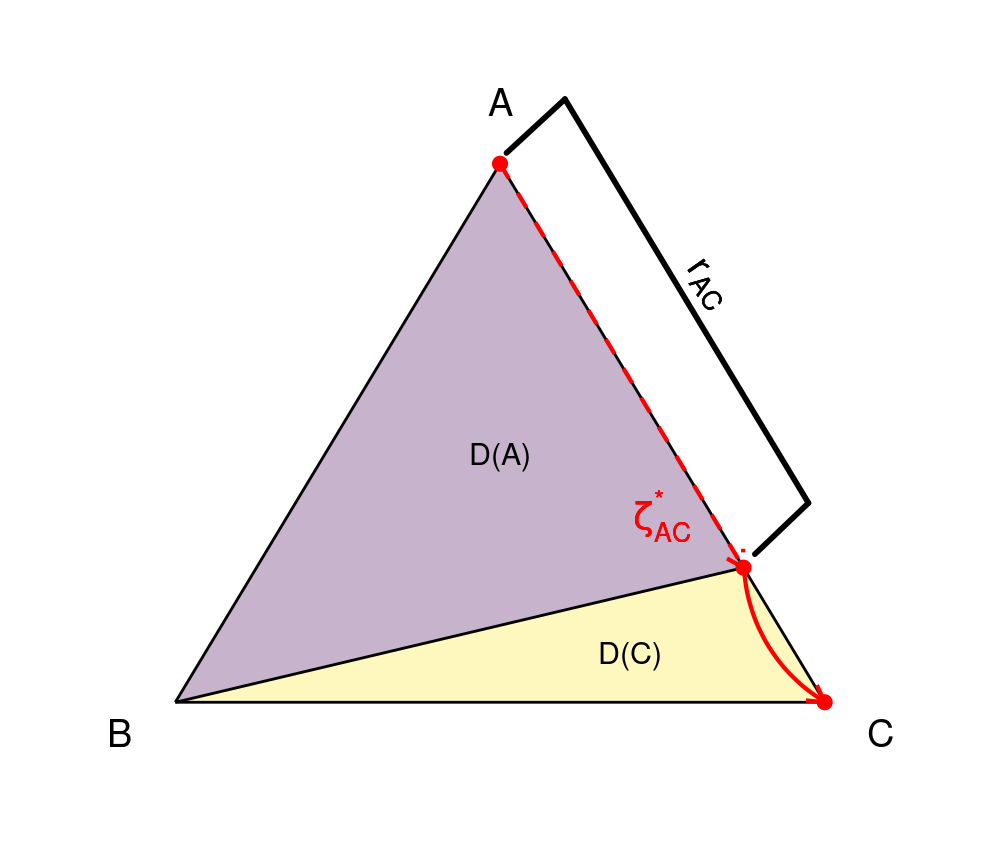
\includegraphics[width = \textwidth]{Images/Tree_1.png}
\end{minipage}
\begin{minipage}[c]{.49\textwidth}
\centering
$B$ is a Stepping Stone from $A$ to $C$
\vskip6pt
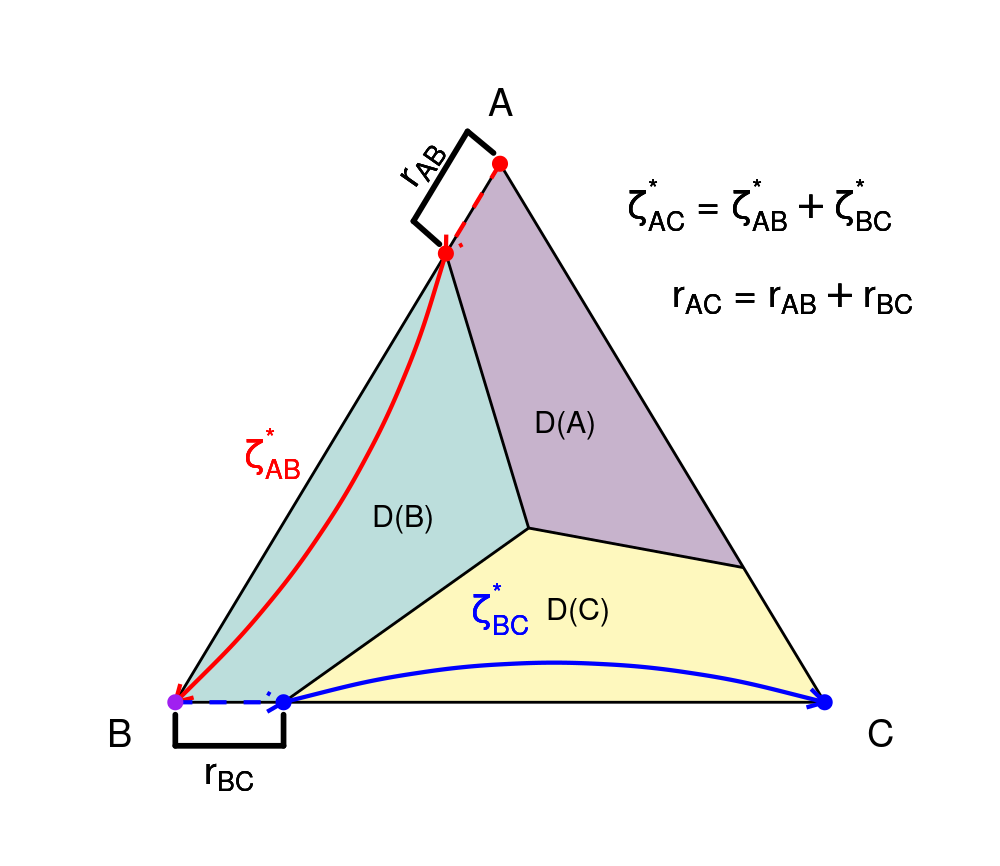
\includegraphics[width = \textwidth]{Images/Tree23.png}
\end{minipage}
\vskip12pt
\small
\centering
In the game on the left there are only 2 recurrent classes: pure strategy equilibria of all $A$ and all $C$. The path of least resistance is to in one step move from $A$ to the nearest point in $D(C)$ and then move from $D(C)$ to $C$ with no added resistance. In the game on the right, the path of least resistance is instead from $A$ to $D(B)$ to $B$ to $D(C)$ to $C$. 
\end{figure}
\justifying
\vskip12pt

Now construct a directed graph with $K$ vertices, one for each recurrent class. Call the vertex corresponding to the recurrent class $E_i$ vertex $i$. The weight on the directed edge from vertex $i$ to vertex $j$ is $r_{ij}$. The tree rooted at vertex $i$ contains $K-1$ directed edges such that there is a pathway from each vertex $j \neq i$ to vertex $i$. The resistance of each rooted tree is calculated as the sum of weights of the $K-1$ directed edges in the tree. 

\begin{definition}
    STOCHASTIC POTENTIAL: The stochastic potential, $\gamma_i$, of a recurrent class $i$ is the tree rooted at $i$ with the lowest resistance.
\end{definition}

\begin{figure}[h]
\captionsetup{justification=centering}
  \caption{Trees rooted at $C$}
   \label{fig:TreesTheory2}
\vskip12pt
\begin{minipage}[c]{.32\textwidth}
\centering
Tree 1
\vskip6pt
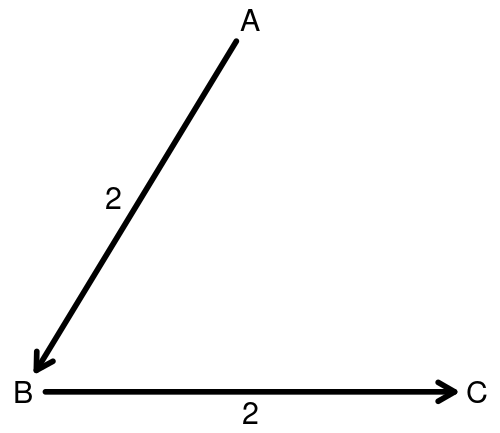
\includegraphics[width = \textwidth]{Images/Tree1.png}
\end{minipage}
\begin{minipage}[c]{.32\textwidth}
\centering
Tree 2
\vskip6pt
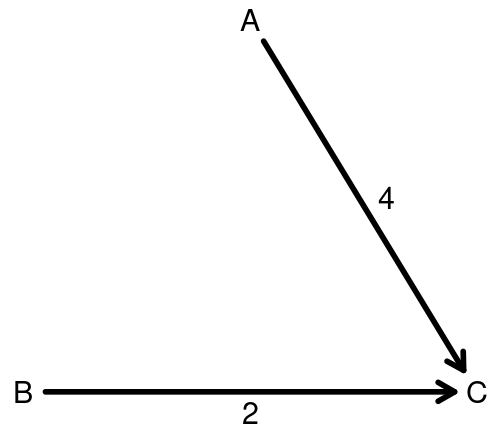
\includegraphics[width = \textwidth]{Images/Tree2.png}
\end{minipage}
\begin{minipage}[c]{.32\textwidth}
\centering
Tree 3
\vskip6pt
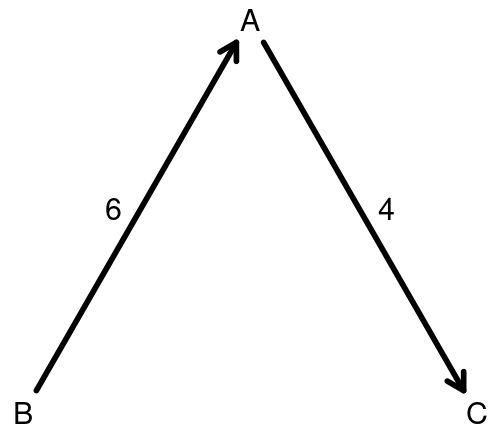
\includegraphics[width = \textwidth]{Images/Tree3.png}
\end{minipage}
\vskip12pt
\small
\centering
In a game with 3 recurrent classes there are 3 vertices, each with 2 directed edges such that there is a pathway from each vertex to $C$. In this example, The resistance of each rooted tree is 4, 6, and 10 for Tree 1, Tree 2 and Tree 3 respectively. As such, the stochastic potential of $\gamma_C$ is 4.  
\end{figure}
\justifying
\vskip12pt

\cite{young1993evolution} showed that the stochastically stable states are those contained in the recurrent class with the minimum stochastic potential in the game. 

\begin{definition}
    STOCHASTIC STABILITY: A state $s$ is stochastically stable if $s$ has the smallest stochastic potential of all states.
\end{definition}

Given that the inclusion of a stepping stone $E''$ in a game reduces the resistance from $E$ to $E'$, stepping stones not only reduce the resistance of directed transitions but may also affect the set of stochastically stable states.

The goal of the experiment is to test if stepping stone equilibria are effective as theoretically predicted. That is to say, that when populations play long repeated games they utilize stepping stones to transition between conventions. In the next section, I describe how I choose the payoffs in each game played in the experiment. 

\subsubsection{Treatment Design}

I design a lab experiment to test if players utilize stepping stones and if so, if there are certain aspects of the game that make a stepping stone more effective. Of particular interest, I study how the strategy profile of the group evolves when playing a coordination game with Pareto-rankable equilibria when the population starts the game at a Pareto dominated equilibrium.\footnote{A game with Pareto-rankable equilibria means that at least one equilibrium is preferred by all players in the game to another equilibrium.} To do this, I use a 2x3 treatment design. 

One dimension of the treatment design is selecting the games groups played. Groups of size 8 were asked to play one of three augmented stag hunt games all of which had groups starting the game playing $E_A$. In two of the three games (Game 2 and 3), a stepping stone was added to the classic stag hunt game. In Game 2 a stepping stone that payoff dominates the starting equilibrium was added. I will refer to this as the high payoff stepping stone treatment. In Game 3 I instead add a stepping stone that is payoff dominated by the starting equilibrium. I will refer to Game 3 as the low payoff stepping stone treatment. The motivation for the different stepping stone levels is to see if payoff dominance in transitions makes a difference in group’s play. In the control game (Game 1), groups played without a stepping stone and instead with an added strategy that guaranteed the worst payoff possible.

On the other dimension of the treatments, I varied the amount of information subjects were given. Players were given either \textit{complete information} meaning that they knew both their payoffs and the payoffs of the other players in the game, or players were given \textit{incomplete information} meaning they did not know what payoffs the other players received for a given strategy profile. This is important since having common knowledge that players are playing a coordination game and are starting at an inefficient equilibrium may impact player’s decisions, presumably by making them more forward looking.

\begin{figure}[h]
\captionsetup{justification=centering}
  \caption{Parameter Selection}
   \label{fig:Parameters}
   \centering
\vskip6pt
\begin{tabular}{cc|c|c|c|}
      & \multicolumn{1}{c}{} & \multicolumn{3}{c}{Player 2}\\
      & \multicolumn{1}{c}{} & \multicolumn{1}{c}{$A$}  & \multicolumn{1}{c}{$B$} & \multicolumn{1}{c}{$C$} \\\cline{3-5}
      \multirow{2}*{Player 1}  & $A$ & $a_G$ & $b_G$ & $e_G$ \\\cline{3-5}
      & $B$ & $c_G$ & $d_G$ & $g_G$ \\\cline{3-5}
      & $C$ & $f_G$ & $h_G$ & $i_G$ \\\cline{3-5}
    \end{tabular}
        \vskip12pt\small
The game is symmetric and the reported payoffs are those of the row player
\end{figure}

I create a $3 \times 3$ symmetric game with action space $\{A, B, C\}$ with the payoffs received by the row player in game $G = \{1, 2, 3\}$ as depicted in Figure~\ref{fig:Parameters} with three pure strategy Nash equilibrium: $E_A = (A, A)$, $E_B = (B, B)$, and $E_C = (C, C)$ in each game. With 9 payoff variables in each game $G$, parameters were chosen to create a large difference in the path of least resistance from $E_A$ to $E_C$ between the game without a stepping stone, Game 1, and the games with a stepping stone, Games 2 and 3, while observing certain restrictions, namely: 

\begin{enumerate}
    \item $E_A$ and $E_C$ must be strict Nash equilibria. Thus, $a_G > c_G, f_G$; $i_G > e_G, g_G$ $\forall G$
    \item $E_B$ must be a strict Nash equilibrium in Games 2 and 3. Thus, $d_i > b_i, h_i$ $i \in \{2, 3\}$
    \item $E_C$ must be the Pareto Efficient equilibrium. So, $i_G > a_G, d_G$ $\forall G$
    \item The variables $a_G, e_G, f_G, i_G$ must remain the same across all games.
    \item The resistance from $E_A$ to $E_B$ must be equal to the resistance from $E_B$ to $E_C$ in and between Games 2 and 3.\footnote{By controlling for the resistance between equilibria between and across games I can test for the effect of pairwise and global payoff dominance.}
    \item In Game 1 (no stepping stone), $b_1, c_1, d_1, g_1, h_1$ must be equal to the lowest payoff in the game.
    \item The variables $a_G$ and $e_G$ must be equal so that Game 1 is essentially a stag hunt game.
    \item $a_G+e_G > f_G+i_G$ so that $E_A$ pairwise risk dominates $E_C$.
    \item In Game 2 (high payoff stepping stone), the payoff at the transition equilibrium must be greater than that at the starting equilibrium $d_2 > a_2$.
    \item In Game 3 (low payoff stepping stone), the payoff at the transition equilibrium must be smaller than that at the starting equilibrium $d_3 < a_3$.
    \item To make calculations as simple as possible for subjects, all payoffs must be single digit integers.
    \item Payoffs must be greater than 0 to avoid behavioral distortions \citep{tversky1991loss, gneezy1997experiment}.
\end{enumerate}

 In all games $E_A$ pairwise risk dominates $E_C$ which implies that $E_A$ is the stochastically stable equilibrium in the 2x2 game with just $A$ and $C$ which is the result of Theorem 4.2 in \cite{Young1998}. This dynamic lends additional justification for initiating the game with everyone playing $A$. 

\subsubsection{Games and Theoretical Analysis}

\vskip12pt
\begin{figure}[h]
\captionsetup{justification=centering}
  \caption{Games Played in the Experiment}
   \label{fig:Games}

    \begin{minipage}[c]{.32\textwidth}
    \centering
    Game 1
    \vskip6pt
    \begin{tabular}{cc|c|c|c|}
          & \multicolumn{1}{c}{} & \multicolumn{3}{c}{Player 2}\\
          & \multicolumn{1}{c}{} & \multicolumn{1}{c}{$A$} 
          & \multicolumn{1}{c}{$B$} 
          & \multicolumn{1}{c}{$C$} \\\cline{3-5}
      \multirow{2}*{Player 1}  & $A$ & $7$ & $1$ & $7$ \\\cline{3-5}
      & $B$ & $1$ & $1$ & $1$ \\\cline{3-5}
      & $C$ & $1$ & $1$ & $9$ \\\cline{3-5}
    \end{tabular}
\end{minipage}
\begin{minipage}[c]{.32\textwidth}
\centering
Game 2
\vskip6pt
\begin{tabular}{cc|c|c|c|}
      & \multicolumn{1}{c}{} & \multicolumn{3}{c}{Player 2}\\
      & \multicolumn{1}{c}{} & \multicolumn{1}{c}{$A$}  & \multicolumn{1}{c}{$B$} & \multicolumn{1}{c}{$C$} \\\cline{3-5}
      \multirow{2}*{Player 1}  & $A$ & $7$ & $3$ & $7$ \\\cline{3-5}
      & $B$ & $6$ & $8$ & $4$ \\\cline{3-5}
      & $C$ & $1$ & $7$ & $9$ \\\cline{3-5}
    \end{tabular}
\end{minipage}
\begin{minipage}[c]{.32\textwidth}
\centering
Game 3
\vskip6pt
\begin{tabular}{cc|c|c|c|}
      & \multicolumn{1}{c}{} & \multicolumn{3}{c}{Player 2}\\
      & \multicolumn{1}{c}{} & \multicolumn{1}{c}{$A$}  & \multicolumn{1}{c}{$B$} & \multicolumn{1}{c}{$C$} \\\cline{3-5}
      \multirow{2}*{Player 1}  & $A$ & $7$ & $1$ & $7$ \\\cline{3-5}
      & $B$ & $6$ & $6$ & $4$ \\\cline{3-5}
      & $C$ & $1$ & $5$ & $9$ \\\cline{3-5}
    \end{tabular}
\end{minipage}
\vskip12pt
\small
\centering

The games are all symmetric and the reported payoffs are those of the row player
\end{figure}
\justifying
\vskip12pt

Figure~\ref{fig:Games} shows the construction of the three different games played in the experiment. All three games are symmetric with the payoffs reported being those of the row player. In addition, players play against the field meaning they are playing against the full distribution of pure strategies of all other players in the population. All 3 games are coordination games with 3 pure strategy Nash equilibria on the diagonal. I will refer to each equilibrium, where all 8 players play the same strategy, as follows: $E_A = (A, A, \dots, A)$, $E_B = (B, B, \dots, B)$, $E_C = (C, C, \dots, C)$. Game 1 represents the case where there is no stepping stone from $E_A$ to $E_C$. Note that Game 1 is essentially a stag hunt game. I include $B$ as a strategy to increase the confidence that any change in play between different games is due to the change in payoffs and not due to a change in the strategy space of the game. As a benefit, including $B$ in game 1 guarantees players will receive the worst possible payoff in the game allow us to test if random errors that don't take into account payoffs occur.\footnote{This is assuming that players don't utilize $B$ as a way to punish other players, or in games with \textit{incomplete information}, use $B$ to see if that may help other players move from $A$ to $C$}

The idea of trying to solve the coordination failure problem as seen in stag hunt games with the addition of another strategy was examined in \cite{cooper1990selection}. However, I differ here by adding a third equilibrium, a stepping stone, to game 2 and 3 instead of a dominated strategy. Note that Game 3 is constructed by taking a payoff transformation of Game 2 that preserves the best reply structure, specifically by subtracting the payoff the row player receives when the column player plays $B$ by 2 \citep{harsanyi1988general}. This transformation allows me to test what, if any, effect payoff dominance for the stepping stone strategy has. In theory, there shouldn't be any difference between individuals whose play is motivated by myopic payoff differences. However, there is reason to believe that player's decisions are also influenced by payoff dominance \citep{harsanyi1988general, jagau2022}.

\subsubsection*{Resistance Calculations}


 In order for the added equilibrium, $E_B$, in Games 2 and 3 to be considered a stepping stone from one equilibrium, $E_A$, to another, $E_C$, the path of least resistance from $E_A$ to $E_C$ must go through an indirect path through $E_B$ compared to the most efficient direct path from $E_A$ to $s \in D(E_A)$ to $E_C$.\footnote{All strict Nash equilibria are recurrent classes in this game.} Simply stated, $E_B$ is a stepping stone if the resistance from $E_A$ to $E_C$ is smaller in Games 2 and 3 than Game 1.


Below I calculate the resistance from $E_A$ to $E_C$ in Games 1, 2, and 3. Refer to Figure~\ref{fig:ResistancePlotsTheory} for a depiction of the directed paths of least resistance on a simplex. Note that the graphs depict the mapping of the strategies of the other players in the group from the perspective of a player who always plays their myopic best response. This distinction is made since players best respond to the other players' strategies and this set of strategies will differ across players if their own strategies are not the same as one another. As such, by examining the best reply structure of a player who always plays their myopic best response, the minimum number of "mistakes" necessary to change the myopic best response of some players, and following that, the entire group is revealed. This is possible because of stochastic strategy updating implemented in this game. The path of least resistance does not necessarily require transitioning directly from $E_A$ to $s' \in D(E_C)$. It is possible to transition from $E_A$ to some $s \in D(E_A)$ then with no further mistakes but with selective stochastic strategy updating, make the transition directly from $s$ to $E_C$. I elaborate below. 

\begin{figure}[h]
\captionsetup{justification=centering}
  \caption{Path of Least Resistance from $E_A$ to $E_C$ in Games 1, 2 and 3}
   \label{fig:ResistancePlotsTheory}

\vskip12pt
\begin{minipage}[c]{.49\textwidth}
\centering
Game 1 
\vskip6pt
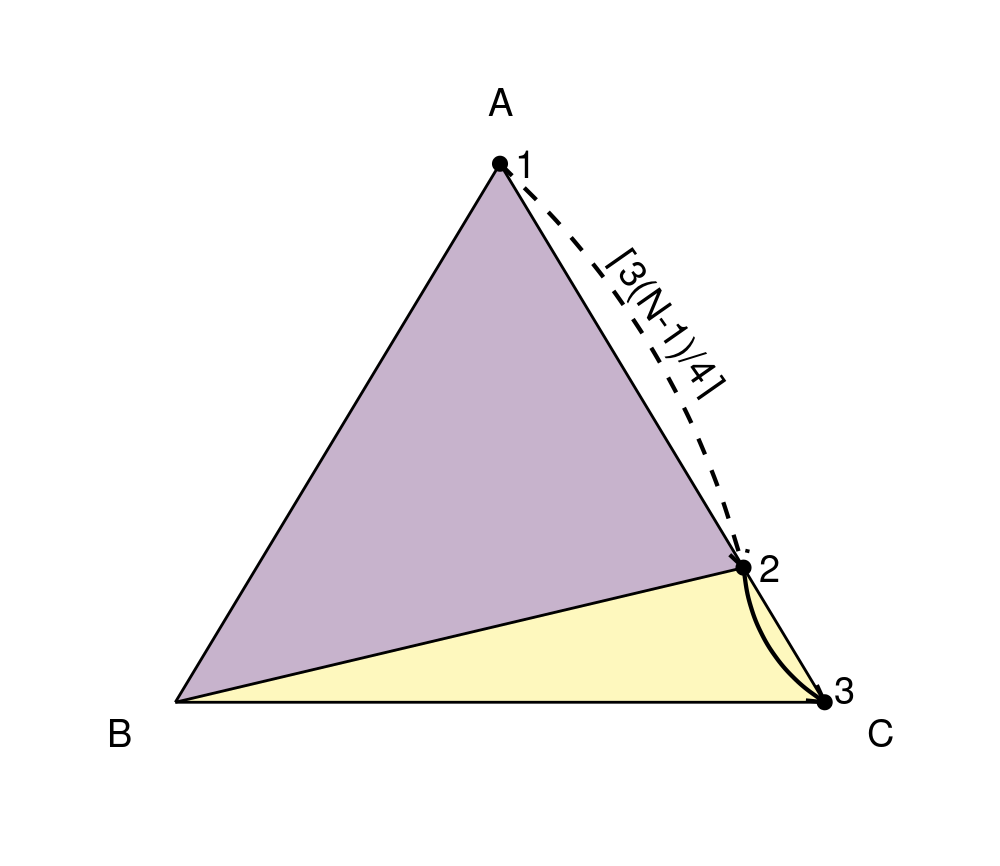
\includegraphics[width = \textwidth]{Images/Resistance1.6.png}
\end{minipage}
\begin{minipage}[c]{.49\textwidth}
\centering
Games 2 and 3 
\vskip6pt
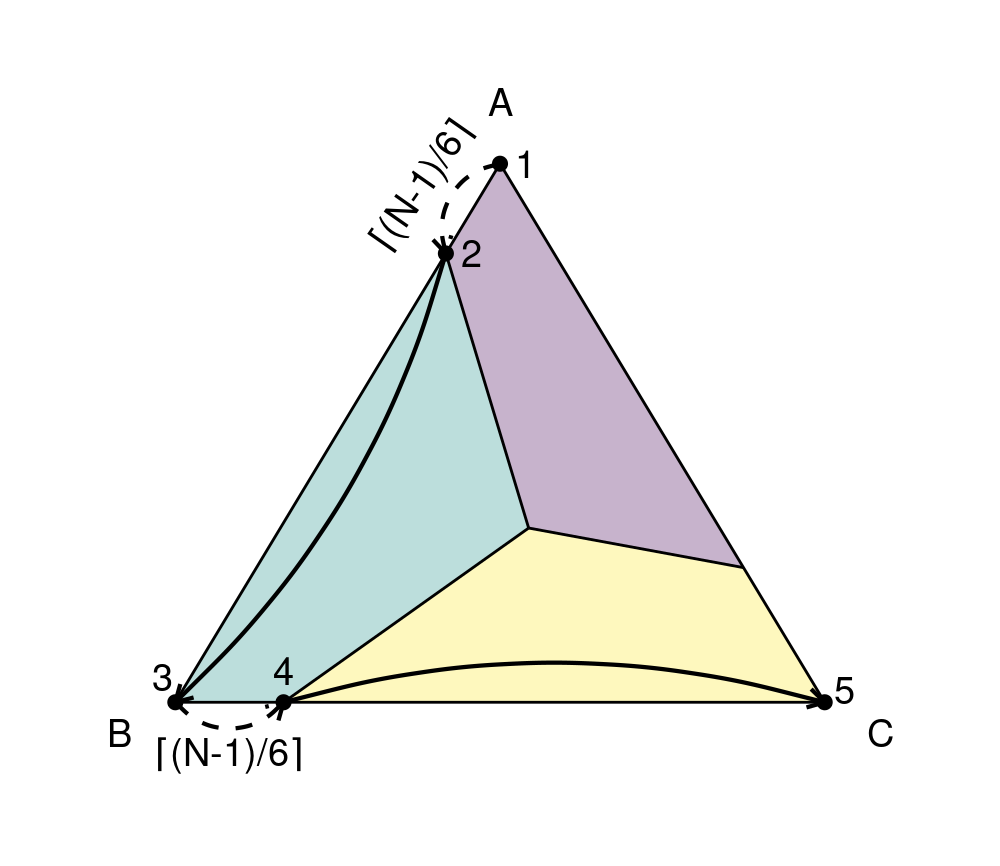
\includegraphics[width = \textwidth]{Images/Resistance23.6.png}
\end{minipage}
\vskip12pt
\small
\centering
Recall: The best reply structure is the same in Games 2 and 3.
Because resistance is a count of only non-myopic best response play (represented by dashed curves), once the game is within the basin of attraction of an equilibrium $D(E)$, it can travel the rest of the way to that equilibrium using only best response play (represented by solid curves). Note that the paths are curved only to make following the steps easier to follow. The directed path accurately mapped onto the simplex is a straight line. The basins of attraction for each recurrent class is color coded in the simplex: purple for $E_A$, green for $E_B$, and yellow for $E_C$.

\end{figure}
\justifying
\vskip12pt

First I will describe the path of least resistance in Game 1, which is also the directed path of least resistance that travels directly from $E_A$ to $E_C$ without entering $D(E_B)$ in Games 2 and 3. Starting from $E_A$ (1) the transition into $D(E_C)$ can be accomplished with the least "mistakes" required by transitioning to a state where $\lceil3(N-1)/4 \rceil$\footnote{The notation $\lceil x \rceil$ means rounding up to the nearest integer that is greater than or equal to $x$.} of the players play $C$ and all other players play $A$, requiring a minimum of $\lceil3(N-1)/4 \rceil$ "mistakes". Once in this state, (2), the remaining $N - \lceil3(N-1)/4 \rceil$ players who have $A$ as their current strategy calculate their expected payoffs for playing against their opponents' last period strategies. If they play $A$ then their expected payoff is $7(N-1)$. If they play $C$ then their expected payoff is $N-1 - \lceil3(N-1)/4 \rceil$ + $9 \lceil3(N-1)/4 \rceil \geq 7(N-1)$. So they can play $C$ as a best response. The other $\lceil3(N-1)/4 \rceil$ players whose current strategy is $C$ have $A$ as their unique best response. Since $\lceil3(N-1)/4 \rceil \geq N/2$ it can be shown that the current state is in $D(E_A)$. However, it is possible that all players whose last period strategy was $A$ now play $C$ and their strategies are all stochastically accepted while all the players last period strategy was $A$ now have their actions stochastically rejected. Hence, $E_C$ (3) is reached. The resistance from $E_A$ to $E_C$ in Game 1 is therefore $\lceil3(N-1)/4 \rceil$.

Now I will describe the path of least resistance in Games 2 and 3. Starting from $E_A$ (1) the transition to a state in $D(E_B)$ can be made by $\lceil(N-1)/6 \rceil$ players picking $B$ as their action by "mistake" and all those actions being stochastically accepted. In the next period (2), the players who did not make a mistake get and expected payoff of $7(N-\lceil(N-1)/6 \rceil) + 3\lceil(N-1)/6 \rceil$ if they pick $A$, $6(N-\lceil(N-1)/6 \rceil) + 8\lceil(N-1)/6 \rceil$ if they pick $B$, and $(N-\lceil(N-1)/6 \rceil) + 7\lceil(N-1)/6 \rceil$ if they pick $C$. Clearly, the expected payoff for $C$ is less than $B$. So $B$ is a best response if $7(N-\lceil(N-1)/6 \rceil) + 3\lceil(N-1)/6 \rceil \leq 6(N-\lceil(N-1)/6 \rceil) + 8\lceil(N-1)/6 \rceil$. The expression simplifies to $N \leq  6\lceil(N-1)/6 \rceil$, so $B$ is a best response. So play can transition to $E_B$ (3) without any additional "mistakes". Once at $E_B$, the transition to a state (4) in $D(E_B)$ can be made by $\lceil(N-1)/6 \rceil$ players picking $C$ as their action by "mistake" and all those actions being stochastically accepted. It is simple to calculate, similar as above, that play can then progress with no further "mistakes" to arrive at $E_C$ (5). Hence, the resistance from $E_A$ to $E_C$ in Games 2 and 3 is $2\lceil(N-1)/6 \rceil$.

As such, the directed paths of least resistance using and not using $E_B$ can now be compared. If $2\lceil(N-1)/6 \rceil < \lceil3(N-1)/4 \rceil$ then $E_B$ is a stepping stone in Games 2 and 3. It is easy to verify that for all $N >3$, $E_B$ is a stepping stone in Games 2 and 3. 


In the experiment, groups of size $N = 8$ were used. As such, $E_B$ is a stepping stone in Games 2 and 3. In all three games, when the game is at $E_A$, the amount of simultaneous deviations from myopic best response needed to make $C$ a best response for the remaining players in the next period is then $\lceil(3/4)*(N-1)\rceil = 6$. In Games 2 and 3, the resistance from $E_A$ to $E_B$ as well as the resistance from $E_B$ to $E_C$ is $\lceil(1/6)*(N-1)\rceil = 2$. Examining the resistance in all three games from $E_C$ to $E_A$ is $\lceil(1/4)*(N-1)\rceil = 2$. In Games 2 and 3, the resistance from $E_C$ to $E_B$ and the resistance from $E_B$ to $E_A$ is $\lceil(1/4)*(N-1)\rceil = 6$. This means if perturbations are independent and payoff independent then if conventions change in Games 2 and 3 they should travel almost exclusively in the direction from $E_A$ to $E_B$ to $E_C$ to $E_A$ et cetera spending on average equal time at each.\footnote{Note that by definition just as $E_B$ is a stepping stone from $E_A$ to $E_C$ so too is $E_C$ a stepping stone from $E_B$ to $E_A$ and $E_A$ is a stepping stone from $E_C$ to $E_B$.} However, if deviations from myopic best response are a function of payoff dominance then populations should spend a greater portion of their time at the payoff efficient equilibrium $E_C$ when cycling or not cycle at all. 


In several evolutionary game theory experiments in the literature \citep{hwang2018conventional, mas2016behavioral}, subjects were randomly given an opportunity to change their strategy in each round. 
In the event they weren't given a revision opportunity, their action from the previous round was retained. 
This is valuable from a data collection standpoint as it slows down the transition from one equilibrium to another, which is where decisions are most important. 
As discussed in the theory section, in this experiment for all games and in every round, all subjects will be asked which action they want to play. 
However, with probability $p$ their new action is adopted and with probability $(1-p)$ their strategy from the previous round is retained.
In essence, in this experiment I am moving the nature node deciding if they can update their strategy from before to after the subject makes their decision. 
This change in procedure yields the benefit of being able to collect $1/p$ times as much data. This procedure is similar to the strategy method \citep{selten1967strategiemethode} which is often used to boost data collection in extensive form games.

For the experiment trails I use $p = 1/2$. The benefit of using a relatively small $p$ value is that it makes states stickier, thus making equilibria more stable. Additionally, it helps enforce the initial condition of all the games in the experiment: that the game starts with everyone playing $A$, corresponding to $E_A$, the safe, payoff dominated equilibrium. This "stickiness" can be demonstrated by considering a player who uses level-K thinking \citep{Nagel1995, stahl1995players}. Consider a level-1 player. They assume every other player plays each strategy with equal probability. So, they expect to face the mixed strategy of $(1-p + p/3, p/3, p/3)$. Thus, since here I use $p = 1/2$, their expected payoffs from playing each strategy is $(36/7, 1, 11/6)$ in Game 1, $(38/7, 36/7, 20/7)$ in Game 2, and $(36/7, 34/7, 18/7)$ in Game 3 for each of strategy $(A, B, C)$ respectively. Thus, $A$ is the unique best response in each game. Level-2 players assume all other players are level-1 players and thus will also play $A$. It follows that for all players of level-$K > 0$ thinking have $A$ as a best response.\footnote{Note that in the \textit{incomplete information} treatment players only know their own payoffs so computing the best responses of other players can not be done reliably, especially at the start of the game.} Now consider if $p = 1$, the case where players are always able to change their strategy. In this case, level 1 thinkers assume they are facing a mixed strategy of $(1/3, 1/3, 1/3)$ which means their expected payoffs from playing each strategy is $(5, 1, 11/3)$ in Game 1, $(17/3, 6, 17/3)$ in Game 2, and $(5, 16/3, 5)$ in Game 3 for each of strategy $(A, B, C)$ respectively. Thus, in Games 2 and 3, $B$ is their best response when $p = 1$ as in this case enforcing that everyone starts the game playing $A$ is little more than a default option \citep{ThalerSunstein08, samuelson1988status}. This example shows how incorporating stochastic strategy updating can affect decisions and enforce initial conditions.  

\subsection{Procedure}
\justifying
18 sessions (3 per treatment) of 8 participants each were held in person at the Tattersall Computer Lab at the University of Oregon. A total of 144 subjects were recruited from the University of Oregon student population, each of which made 200 decisions over the course of one hour and were paid, on average, $\$21$. 

Each participant was seated at a computer with dividers between the monitors and all participants were seated facing a wall to prevent any in-person interaction or viewing of others' screens. The software used for the experiment was built using oTree \citep{chen2016otree}, which is software using Python, HTML, and JavaScript designed for use in laboratory and field experiments in game theory.

The instructions, quiz questions, and screenshots of the UI during the experiment can be found in the appendix.


\subsubsection*{Phase I}
Upon entering the lab and filling out consent forms, participants were read aloud instructions explaining how the game works and how the experiment is conducted. Typed instructions were also be visible on their computer.\footnote{I did not read aloud the payoff tables in order to preserve the \textit{imperfect information} treatment.}

\subsubsection*{Phase II}
Participants were provided with a writing utensil, a basic calculator, and blank paper to make notes and calculations if they desired to use them. After reading the instructions, participants took a short quiz for comprehension to ensure that they understand how the game works and how their payouts would be calculated.
Participants had to answer each question correctly before they could proceed to the following question. The number of errors made by each participant was tracked.

\subsubsection*{Phase III}

Participants then played the experiment which comprised of two sets of 100 rounds each. During each round, participants were able to view the payoff they earned in the previous round, the strategies played by the other participants in the previous round, if their action last round was accepted or rejected, the remaining time lest in the round, their payoff table, and depending on the treatment of the study, their opponents payoffs in the payoff table. In each round, participants were be able to change their strategy with probability = .5 otherwise, their previous round strategy was retained. Everyone started the experiment coordinating on $A$.
In the first two rounds of each set, participants had 60 seconds to pick a strategy. In rounds 3-5, participants had 45 seconds to pick a strategy, In rounds 6-8, participants had 30 seconds to pick a strategy, in rounds 9-11, participants had 20 seconds to pick a strategy, and in rounds 12-200 participants had 10 seconds to pick a strategy. This shrinking decision time is commonly used in similar evolutionary experiments \citep{lim2016experimental, hwang2018conventional}. Failure to select a strategy in a round resulted in the player's previous round strategy being selected for them. The amount of time it took a participant to select their choice in each round was also recorded.

During the first set of 100 rounds, the group played their treatment game (either Game 1, Game 2, or Game 3). After the conclusion of the first set of 100 rounds the participants were brought to an screen informing them of possible changes that were being made to their payoff table for the second set of rounds. Every group played Game 1 in the second set of rounds. However, the treatment of revealing/concealing the other players' payoffs was maintained for each group across sets. 

\subsection{Hypotheses}

\vskip12pt
\textbf{Hypothesis 1}: In the sessions where players play a game where $E_B$ is a stepping stone (Games 2 and 3), the groups will be more successful in making a transition from $E_A$ to $E_C$ than the sessions where $E_B$ is not a stepping stone (Game 1).
\vskip6pt
\begin{quote}
This hypothesis is to test if stepping stone equilibria actually work as predicted: to reduce the amount of time it takes to transition from $E_A$ to $E_C$ by creating a path of lower resistance. Under all arms of the study with a stepping stone, both $\max(r_{AB}, r_{BC})$ and $r_{AB}+r_{BC}$ is less than the direct transition $r_{AC}$, meaning transitions from $E_A$ to $E_C$ are theoretically more probable in Games 2 and 3 than in Game 1.
\end{quote}

\vskip12pt
\noindent
\textbf{Hypothesis} $\boldsymbol{2_0}$: In the games with stepping stones (Game 2 and 3), players will spend the same number of periods with each action as their myopic best response. 
\vskip6pt
\noindent
\textbf{Hypothesis} $\boldsymbol{2_A}$: In the games with stepping stones (Game 2 and 3), players will spend a plurality of the periods played with the action corresponding to the Pareto efficient equilibrium as their myopic best response.

\begin{quote}
As discussed when calculating resistances, since the weight on the directed edges from vertex $A$ to $B$, $B$ to $C$, and $C$ to $A$ are then same when $N = 8$, if "mistakes" are uniformly random then each state $E_A$, $E_B$, and $E_C$ are stochastically stable. Which means that the adaptive process is expected to spend an equal time at each equilibrium.

However, if deviations from myopic best response are a. payoff dependant or b. a function of equilibrium payoff dominance then populations should spend a greater portion of their time near the Pareto efficient equilibrium, $E_C$. This is because a. The cost per game played of the first deviation from $A$ to $B$ and $B$ to $C$ is only 1, where as the cost per game played of the first deviation from $C$ to $A$ is 2.\footnote{I remind the reader that each player plays the game against all other players in each round.} The explanation for preference for playing the payoff dominant equilibrium, b., is self-evident.

\end{quote}

\vskip12pt
\noindent
\textbf{Hypothesis} $\boldsymbol{3_0}$: The rate of deviations from the myopic best response of $A$ to choosing action $B$ will be no higher when the stepping stone payoff dominates the starting equilibrium (Game 2 vs Game 3).
\vskip6pt
\noindent
\textbf{Hypothesis} $\boldsymbol{3_A}$: The rate of deviations from the myopic best response of $A$ to choosing action $B$ will be higher when the stepping stone payoff dominates the starting equilibrium (Game 2 vs Game 3). 

\begin{quote}

The theoretical prediction under uniform random errors is that the transition dynamics of these games should be identical since the resistance between equilibria are the same in Games 2 and 3. Myopic payoff dependant deviations also produces the same prediction since when comparing Game 2 to Game 3, the expected payoffs increase by the same amount, depending on how many other players play $B$, for all strategies a player can choose from. 

However, there is reason to believe the transition speed may be faster in Game 2 than Game 3. This is because in Game 2 $E_B$ payoff dominates $E_A$ where $E_A$ payoff dominates $E_B$ in game 3. In essence, this hypothesis tests if deviations from a myopic best response towards a stepping stone are a function of payoff dominance.

\end{quote}

\vskip12pt
\noindent
\textbf{Hypothesis} $\boldsymbol{4_0}$: Deviations from myopic best response are payoff independent.
\vskip6pt

\noindent
\textbf{Hypothesis} $\boldsymbol{4_A}$: Deviations from myopic best response are payoff dependant and occur less frequently as the difference between expected payoff of the myopic best response and the next highest expected payoff increases.
\vskip12pt

\vskip12pt
\noindent
\textbf{Hypothesis} $\boldsymbol{5_0}$: Strategy update success will not influence rate of deviation from myopic best response.

\vskip6pt
\noindent
\textbf{Hypothesis} $\boldsymbol{5_A}$: Strategy update success will increase rate of deviation from myopic best response.


\begin{quote}

Although update probability is constant and independent, subjects who recently experienced a low update success rate may view deviations as riskier behavior.

\end{quote}

\noindent
\textbf{Hypothesis} $\boldsymbol{6_0}$: In Game 1, $1/2$ of the "mistakes" made are players choosing action $B$.
\vskip6pt
\noindent
\textbf{Hypothesis} $\boldsymbol{6_A}$: In Game 1, less than $1/2$ of the "mistakes" made are players choosing action $B$.

\begin{quote}
    This hypothesis is similar to hypothesis 4, but the result is more straightforward since there are few ways to rationalize playing $B$ in Game 1. If $B$ accounts for significantly less than half of the "mistakes" then we have evidence that "mistakes" are not uniformly distributed.
\end{quote}




\vskip12pt
\noindent
\textbf{Hypothesis} $\boldsymbol{7_0}$:  The rate of deviations from the myopic best response when the myopic best response does not correspond to the Pareto efficient equilibrium will be equal across games with \textit{complete information} vs \textit{incomplete information}.
\vskip6pt
\noindent
\textbf{Hypothesis} $\boldsymbol{7_A}$:  The rate of deviations from the myopic best response when the myopic best response does not correspond to the Pareto efficient equilibrium will be higher in games with \textit{complete information} vs \textit{incomplete information}.

\begin{quote}

Under \textit{incomplete information}, it will take sophisticated subjects time to realize that this is a coordination game, if in fact they do, and they may never realize that their payoffs align in such a way that $E_C$ is Pareto efficient and that $E_B$ is a stepping stone from $E_A$ to $E_C$.


If players have \textit{complete information}, however, they will immediately know that this is a coordination game and that $E_C$ is an equilibrium and the Pareto efficient outcome. Consequently, a deviation from an equilibrium may be viewed by other players as a costly signal towards a new equilibrium.

If subjects are sufficiently sophisticated, they will realize in Games 2 and 3 that using $E_B$ as a stepping stone is a more efficient path towards $E_C$ than just going directly from $E_A$ to $E_C$, both in terms of payoff forgone in the transition, and the number of likewise deviations needed to shift the myopic best response. However, some players may instead view the direct jump as a faster method of transitioning. In either case, their rate of deviation from myopic best response when the myopic best response isn't $A$ should be higher than the groups with the \textit{incomplete information} treatment.

If this hypothesis is true, then \textit{complete information} should have an attenuation effect of the amount of time it takes to transition from one equilibrium to the next.

\end{quote}

\section{Experimental Results}

\subsection{Group Level Results}


\subsubsection*{Stepping Stone vs. No Stepping Stone}
The primary goal of the experiment was to test if the inclusion of a stepping stone equilibrium was effective in facilitating the transition from the initial equilibrium, to the Pareto efficient equilibrium. Here I discuss the first set of each experiment during which groups played one of three games for 100 rounds: Game 1 which had no stepping stone, Game 2 which had a high payoff stepping stone, and Game 3 which had a low payoff stepping stone. 

Figure \ref{fig:Set1} shows the evolution of groups' strategies in the first 100 rounds of 6 different sessions, one from each treatment. If the stepping stones were effective in facilitating transitions from $A$ to $C$ then Groups playing a game with a stepping stone should make it to $E_C$ with higher probability and  consequently, spend more rounds playing $C$.

I find that in all 12 sessions where groups played with a stepping stone they were able to, at least once, make it to $E_C$. By contrast, in the 6 sessions where players played Game 1 in the first set, only 4 groups were able to make it to $E_C$. I test Hypothesis~1 using a 1-sided Fisher's Exact Test which yields a $p$-value = 0.09804. While this is above the $.05$ threshold traditionally required to reject that groups are just as likely to reach $E_C$ when playing Game 1, it does support the idea that stepping stones are effective as theoretically predicted.   

Beyond the binary of "did a group transition to $E_C$?", the proportion that each strategy was played can be analyzed. Table \ref{tab:propstrateach} reports the proportion that each strategy was played in each experiment. Note that in $4/6$ of the sessions with no stepping stone $A$ accounted for the majority of strategies in set 1. This is in sharp contrast to the games played with a stepping stone where $C$ made up the plurality of the strategies in every experiment. I use a mixed logistic regression with clustering at the individual and experiment level, the results of which can be found in Table \ref{regression:logit1}, which show that players played $C$ in Game 2 and Game 3 significantly more than in Game 1. 

\begin{figure}[H]
  \captionsetup{justification=centering}
  \caption[caption]{Time Series of Group Strategy in Set 1 (Treatment)}
  \makebox[\textwidth][c]{\hspace{10pt} Complete Information Games \hspace{70pt} Incomplete Information Games}
  \label{fig:Set1}
  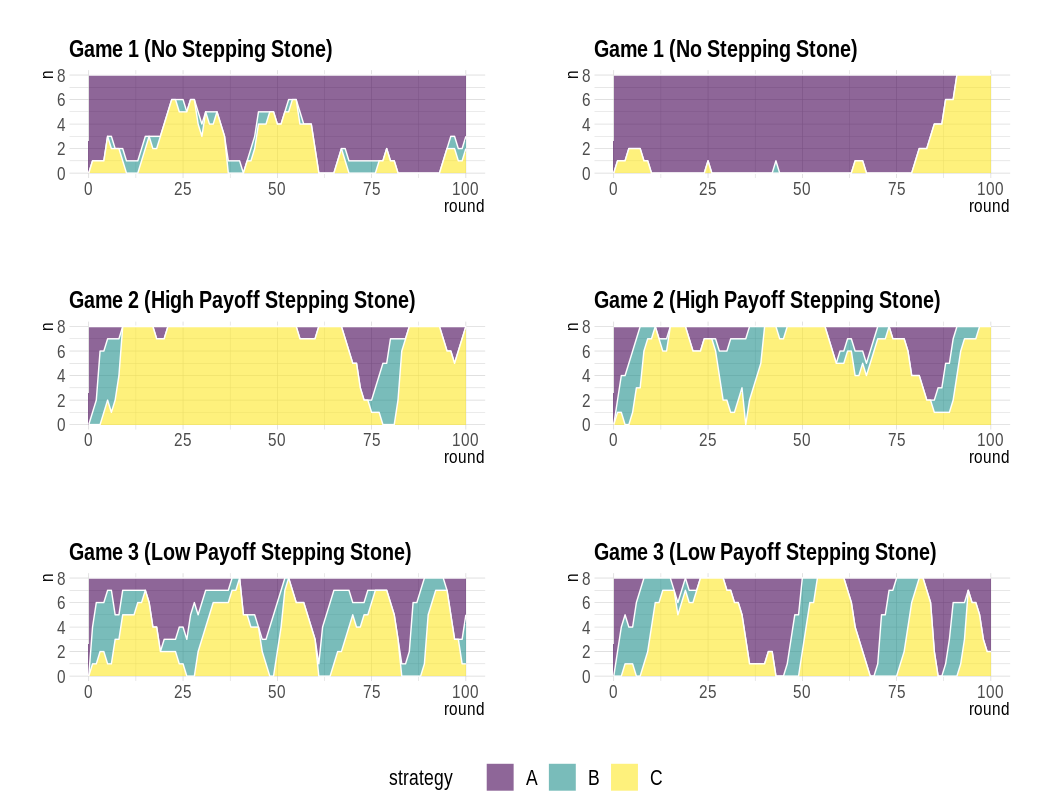
\includegraphics[width=\textwidth, height=340px]{Images/AllAreaPlotSet1_2.png}
  These stacked area plots depict how the proportion of each strategy played changed as the round number increased. The proportion that a strategy was played in a given round is equal to the vertical length with that strategy's color code. The time series of each set of each experiment can be found in the appendix. 
\end{figure}



\subsubsection*{High vs Low Payoff Stepping Stones}

I've established that stepping stones were effective, here I examine if there was a difference in the effectiveness of the low payoff stepping stone compared to the high payoff stepping stone. Looking again at the regression in Table \ref{regression:logit1}, Game 2 had a point estimate of $1.8157$ and Game 3 had a point estimate of $.8588$. Both with standard errors approximately $.31$, this is a large and significant difference between the two, indicating that $C$ is significantly more likely to be played in the sessions with a high payoff stepping stone compared to a low payoff stepping stone. 

Looking at the frequency of strategy played is informative but doesn't provide much insight into the frequency with which strategy profiles were played. Figure \ref{fig:Games23FreqPlot} does just that. In Figure \ref{fig:Games23FreqPlot} and Figure \ref{fig:GamesCIFreqPlot}, I map the strategy profile faced by each player each round onto a simplex, linearly interpolate between the nearest points to flesh out the graph, then color code by frequency, standardized across plots so they can be compared. I also report the frequency that each action is a myopic best response (mBR) to the strategy faced. As can be seen in the Figure \ref{fig:Games23FreqPlot}, play is much more concentrated around $E_C$ in the games with a high payoff stepping stone compared to the games with a low payoff stepping stone. In fact, in the games with a low payoff stepping stone, $A$ and $B$ were myopic best responses twice as often as they were in games with a high payoff stepping stone.

\begin{figure}[h]
\captionsetup{justification=centering}
  \caption{Frequency of Strategy Profile Faced}
   \label{fig:Games23FreqPlot}
    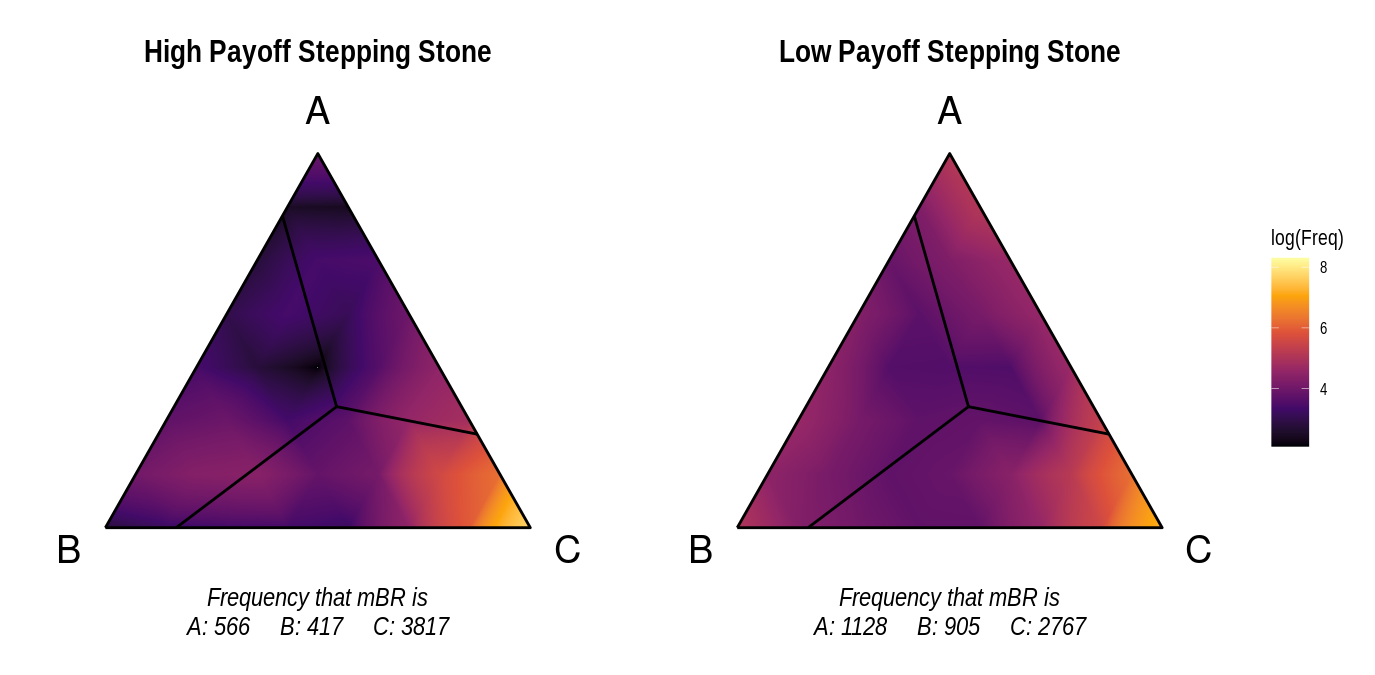
\includegraphics[width = \textwidth]{Images/Games23FreqPlot.png}
\end{figure}

Figure \ref{fig:Games23FreqPlot} illustrates one of Hypothesis 2, which examines whether players in games with stepping stones (Game 2 and 3) spend the same number of periods with each action as their myopic best response. In the sessions, players were observed to have as their myopic best response action $A$ 1694 times, action $B$ 1322 times, and action $C$ 6584 times. 

I conduct a chi-squared test to see if this difference is significant. I get \textit{X}-squared = 5389.5 with 2 degrees of freedom, which reveals a highly significant $p$-value of less than $2.2e^{-16}$. This provides strong evidence which indicates that in Games 2 and 3, players tend to spend more time with $C$, the action corresponding to the Pareto efficient equilibrium as their myopic best response. It is noteworthy that despite the fact that all three states are stochastically stable under uniform perturbations, players exhibit a preference for the Pareto dominant equilibrium.

\subsubsection*{Complete vs Incomplete Information}

\begin{figure}[h]
\captionsetup{justification=centering}
  \caption{Frequency of Strategy Profile Faced}
   \label{fig:GamesCIFreqPlot}
    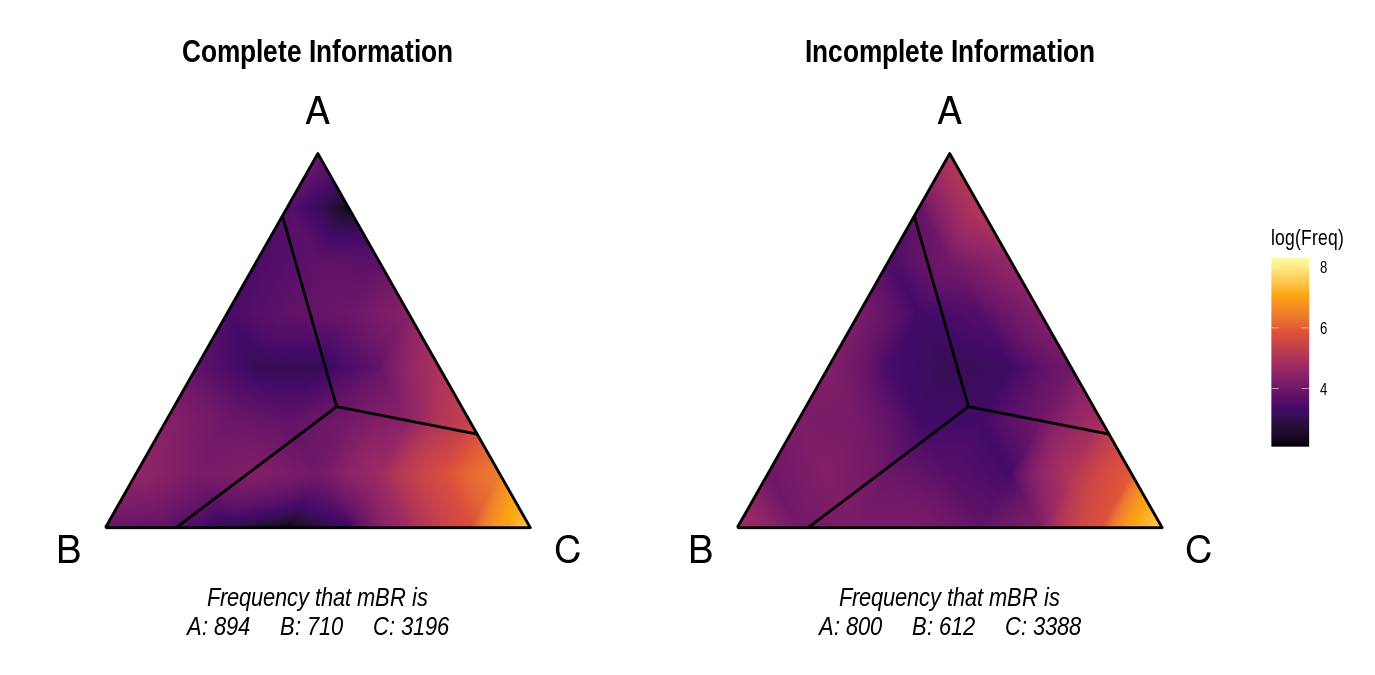
\includegraphics[width = \textwidth]{Images/GamesCIFreqPlot.png}
\end{figure}

When comparing groups that played with a stepping stone with \textit{incomplete information} to those who played with a stepping stone with \textit{complete information}, in aggregate as in Figure \ref{fig:GamesCIFreqPlot} the results appear almost identical. Summary tables \ref{tab:propstrateach} and \ref{tab:propstratall} hint towards the biggest difference between games played with \textit{complete information} vs \textit{incomplete information} are when there are no stepping stones present. During the first 100 rounds, players played $A$ with the highest frequency every time (n=3) when they played Game 1 with \textit{incomplete information}. By contrast, in two of the three sessions with \textit{complete information}, groups were able to make the transition and play $C$ for the majority of the set. The explanation for this is essentially that in \textit{complete information} games players know that they are playing a coordination game and that it is in the group's best interest to transition to $E_C$. As such, it reasons that groups may have a higher propensity to play $C$ even if $A$ is the best response as playing $C$ would likely be viewed as a signal that the player wants to move the group to $C$ and is willing to pay the upfront cost. 

It is perhaps because the barrier to transition out of $A$ was so reduced by the stepping stone that there doesn't appear to be much difference between the complete and \textit{incomplete information} treatments with stepping stones. In this sense, one could think that stepping stones are particularly useful for attenuating the difficulty in coordinating inherent to some environments and populations. 

\subsubsection*{Patterns of Play}

There were two primary patterns of group play observed once a group made the transition to $C$. The group would then either stay at $C$ for the remainder of the set, or would fall into cyclical behavior of playing $A \rightarrow B \rightarrow C \rightarrow A \rightarrow \dots$ until the end of the set. Naturally, those who played Game 1 never fell into the cyclical behavior since playing $B$ guarantees the worst payoff possible. However, more than that, groups who played Game 1 and made it to $E_C$ were the most stable, perhaps recognizing that getting back to $C$ would be difficult if they deviated.

More interestingly, several of the experiment with stepping stones exhibited cyclical behavior. This occurred most frequently in games with \textit{incomplete information} and games with a low payoff stepping stone. There doesn't seem to be a clear reason for why the cyclical process gets initiated, perhaps due to boredom or competitive behavior.\footnote{\cite{sheremeta2010experimental} has shown that in contests with a prize of zero some subjects are still willing to bid to "win".} However, once the process back to $A$ starts, other subjects are quickly pressured by the payoffs to transition as well. From $A$ they transition back to $C$ through $B$. This cyclical behavior creates a positive feedback loop through players expectations. Players learn that play moves from $A$ to $B$ to $C$ to $A$ and the stochastic updating probability encourages players to make decisions based on where they think play is heading least they get left behind and punished. This dynamic should be particularly pronounced in games with \textit{incomplete information} as individuals start the game with no basis for strong prior beliefs as to how their opponents will play. Thus, if they see cycling, they may think they are not playing a coordination game. 

\subsubsection*{Set 2 Results}

After playing 100 rounds of either Game 1, Game 2, or Game 3, all groups played Game 1 (no stepping stone) for the second set of 100 rounds to see if playing with the stepping stone had any effect. For example, can using stepping stones as a crutch in the short term foster long term coordination in other games between the same population? 

Overall, I do not find evidence of correlation between the treatment in the first set and the performance in the second set. Of the eighteen groups, ten of them made it to $E_C$ in the second set with three of the groups having played Game 1 in set 1, four having played Game 2, and three having played Game 3. Four of the ten groups were playing with \textit{complete information} and the remaining six with \textit{incomplete information}. 

What appears to be the biggest predictor of success, meaning making it to $E_C$ and staying there, is if the group ended the previous set at $E_C$. Although every groups' strategy profile was reset to $E_A$ at the start of set 2, none of the groups who ended set 1 with a strategy profile not $E_C$ were able to make it to and stay at $E_C$ in the second set. By contrast, of the twelve groups who did end set 1 at $E_C$, eight of them made it back to and stayed at $E_C$ in set 2.

This effect was driven by the groups with \textit{incomplete information} where across all three games, every group except for one (5/6) that ended at $E_C$ in set 1 ended at $E_C$ in set 2. Among the three groups with \textit{incomplete information} that didn't end set 1 at $E_C$, none of them made it to $E_C$ in set 2. This result is significant under Fisher's Exact Test yielding a $p$-value of 0.04762.


\subsection{Individual Level Results}

At the individual level, I am examining the decisions made by each player. In particular, I examine the rate of myopic best response at different positions in the game and test my remaining hypotheses. Table \ref{tab:choiceexperiment} shows the choices made in each experiment by mBR and table \ref{tab:groupedchoicetreat} shows the aggregated choices by mBR. As expected, most frequently subjects played their myopic best response with a few notable exceptions: in 3 treatments action $A$ was selected as a myopic best response less than half the time. This occurred in both treatments of the high payoff stepping stone game, and in the \textit{incomplete information} treatment of the low payoff stepping stone game. 


\begin{figure}[h]
\captionsetup{justification=centering}
  \caption{Choices in High Payoff Stepping Stone Games}
   \label{fig:Game2ChoiceFreq}
    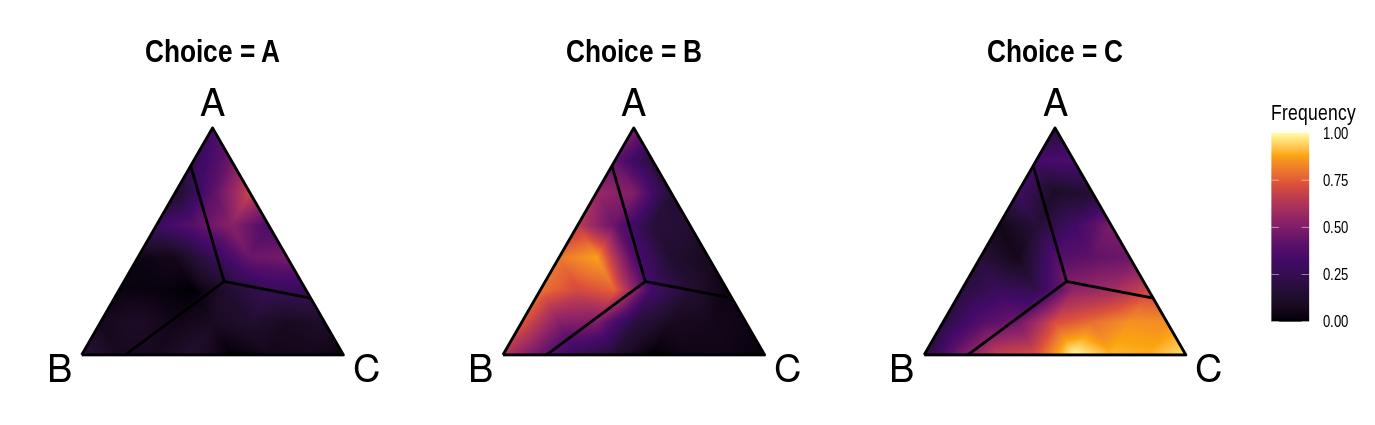
\includegraphics[width = \textwidth]{Images/Game2ChoiceFreq.png}
\end{figure}

\begin{figure}[h]
\captionsetup{justification=centering}
  \caption{Choices in Low Payoff Stepping Stone Games}
   \label{fig:Game3ChoiceFreq}
    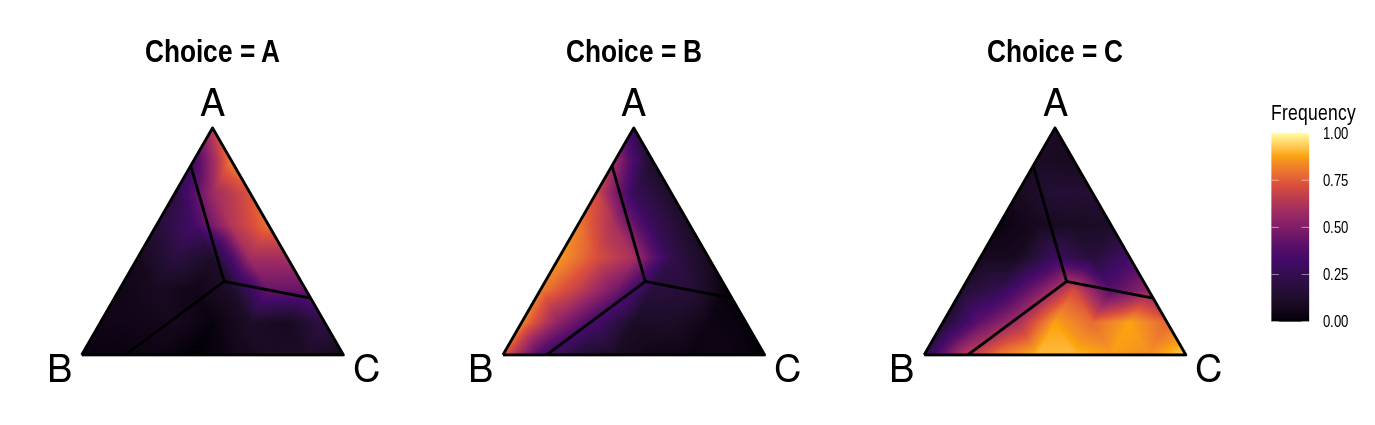
\includegraphics[width = \textwidth]{Images/Game3ChoiceFreq.png}
\end{figure}

\begin{figure}[h]
\captionsetup{justification=centering}
  \caption{Choices in Complete Information Games with a Stepping Stone}
   \label{fig:GameCChoiceFreq}
    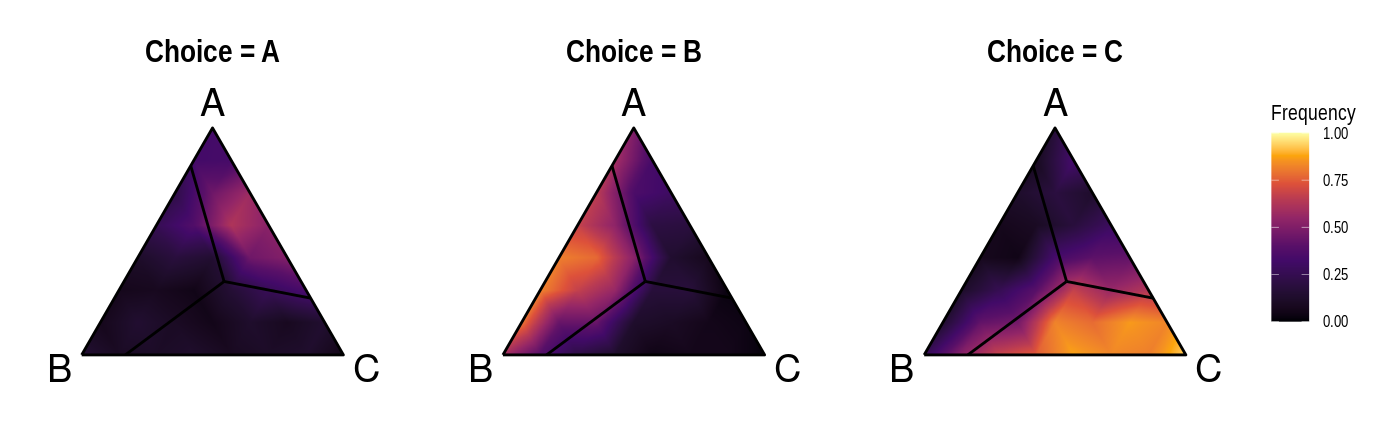
\includegraphics[width = \textwidth]{Images/GameCChoiceFreq.png}
\end{figure}

\begin{figure}[h]
\captionsetup{justification=centering}
  \caption{Choices in Incomplete Information Games with a Stepping Stone}
   \label{fig:GameIChoiceFreq}
    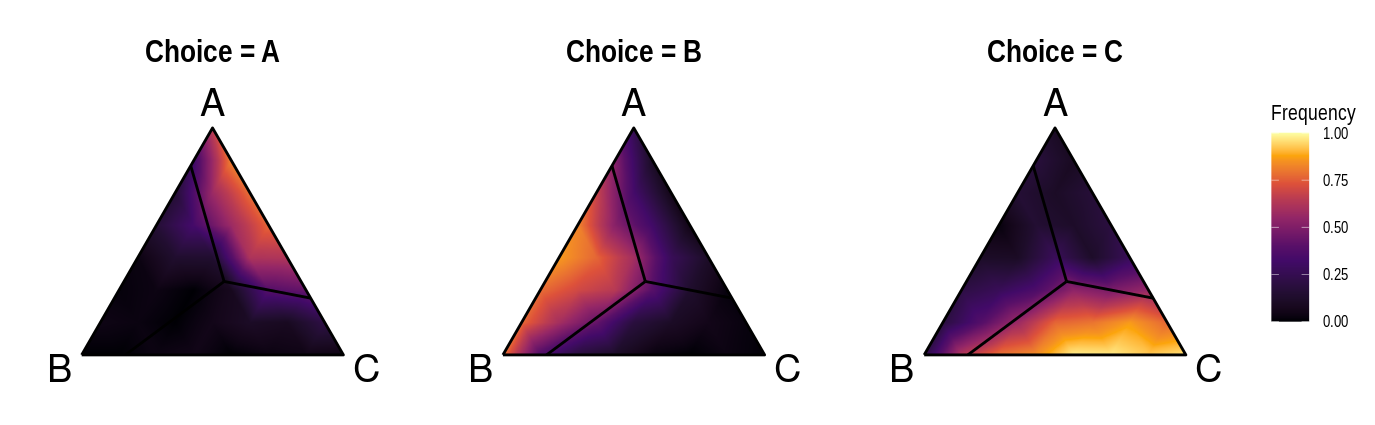
\includegraphics[width = \textwidth]{Images/GameIChoiceFreq.png}
\end{figure}

As discussed in the previous section, these are clear difference in play between Games 2 and 3. Recall, the difference between Game 2 and Game 3 is that in Game 2 the row player's payoff increases by 2 when the column player plays B;\footnote{and because the game is symmetric, the column player's payoff also increases by 2 when the row player plays B} As a result, in Game 2 $E_B$ payoff dominates $E_A$ and in Game 3 $E_A$ payoff dominates $E_B$. Since Game 3 is just a payoff transformation of Game 2 that preserves the best reply structure, theoretically, there shouldn't be any difference between individuals whose play is motivated by myopic payoff differences. As such I hypothesised that the biggest difference would be in the transition from $A$ to $B$ as there is evidence that payoff dominance between equilibria plays a role in players\textquotesingle{} choices \citep{harsanyi1988general, jagau2022}.

I investigate hypothesis 3 by using a generalized logistic mixed model with individual fixed effects to test if the rate of deviation from the myopic best response of $A$ to choosing action $B$ varies significantly across Games 2 and 3. See Table \ref{tab:regression4} for regression results. 

The analysis reveals a difference between the estimates for Game 2 (intercept) and Game 3. The estimated difference is $-0.1030$. The p-value associated with this difference is $0.697$. As result, this test provides no evidence that the rate of deviations towards the stepping stone are payoff dominance dependant. So I can not reject the null hypothesis $3_0$.

Figures \ref{fig:Game2ChoiceFreq}-\ref{fig:GameIChoiceFreq} show the proportion of choices made given the strategy profile faced in different treatments. The graphs were constructed in a similar manner to Figures \ref{fig:Games23FreqPlot} and \ref{fig:GamesCIFreqPlot}, by linearly interpolating across the simplex. The groups that played with a high payoff stepping stone or with \textit{complete information} played $A$ with much lower frequency than those in \textit{incomplete information} games and low payoff stepping stone games. When comparing the high payoff stepping stone to the low payoff stepping stone this result may be explained by $E_A$ Pareto ranking higher in the low payoff stepping stone game.\footnote{$E_A$ payoff dominates $E_B$ in Game 3.} On the information side, the difference in play can be explained by the uncertainty that a better outcome is stable and not being able to observe an efficient path to achieve it. When there is common knowledge of the game, decisions are more likely to be interpreted as intentional signals and players are likely to believe that others will want to transition to $C$ as fast as possible.

Next, I look at what factors influence players to deviate from playing their myopic best response. Figure \ref{fig:Games23MBRPlot} shows the difference in myopic best response play between Game 2 and Game 3 and Figure \ref{fig:GamesCIMBRPlot} shows the difference in myopic best response play between stepping stone games with \textit{complete information} vs \textit{incomplete information}. Across games and levels of information, when players had $C$ as their best response, the strategy corresponding to the Pareto efficient equilibrium, they played their myopic best response 87-91\% of the time, which is inline with the literature examining myopic best response in evolutionary experiments \citep{hwang2018conventional, mas2016behavioral, lim2016experimental}. However, when another strategy was a best response this rate fell dramatically. 

This significant drop off appears to be largely driven by players picking $C$ which partially explains the difference in myopic best response play between when $A$ was the myopic best response and when $B$ was the myopic best response. This is because, by formulation, the basin of attraction for $A$ can contain many more players with the strategy $C$ than the basin of attraction for $B$ can.


I employ a generalized logistic mixed model to examine which factors affect the rate of myopic best response play. I control for the effect that different myopic best responses have on the propensity to play those best responses, as there is a clear difference demonstrated in Figure \ref{fig:Games23MBRPlot}. I also control for the game played and I incorporate clustering at the subject ID level and within the nested experiment number to address potential correlations within the data.
With these controls, I test if there is any significant interaction between \textit{incomplete information} and which strategy is the myopic best response, if the difference in payoff between the myopic best response and the next highest myopic payoff (denoted $\Delta\Pi_{mBR}$), and if past stochastic rejection of strategy updating has any effect on myopic best response play. 

\begin{figure}[h]
\captionsetup{justification=centering}
  \caption{Residual Effect of Round and Lagged Failed Stochastic Update on Choice = mBR Probability}
   \label{fig:Residual}
\vskip12pt
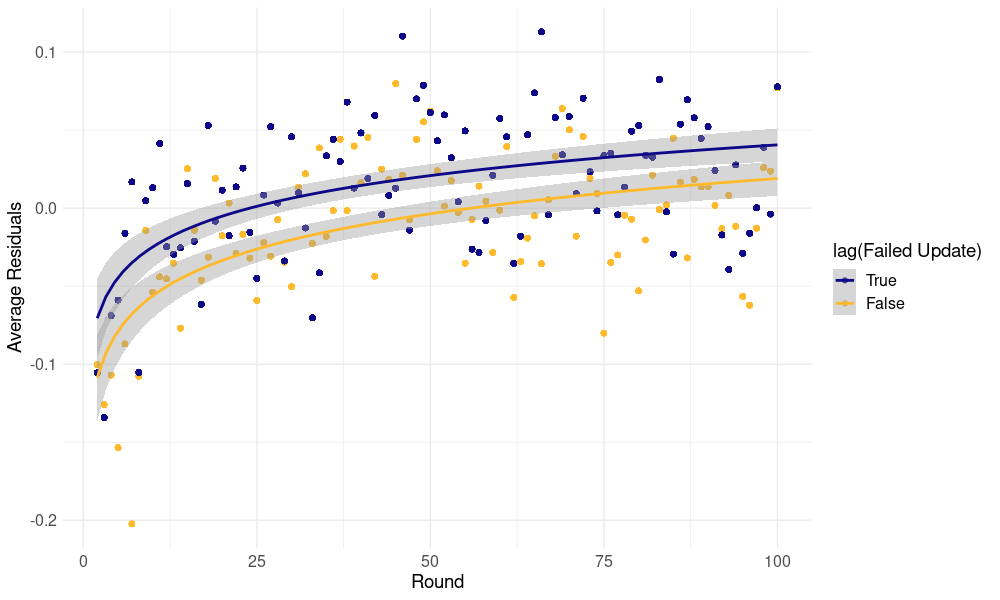
\includegraphics[width = \textwidth]{Images/ResidualPickMBR_round_lagChange.png}
\end{figure}

To account for previous findings of \cite{lim2016experimental} who found a positive influence of the round number on the rate of myopic best response play, I included it as a control variable. To test the most appropriate way to model the effect of round number on subjects choosing to play their myopic best response I regress upon the above specified model excluding the independent variables round and lagged stochastic rejection. I then use the results of the restricted model to predict the probability that subjects will play a myopic best response and graph the residuals in Figure \ref{fig:Residual}. In Figure \ref{fig:Residual}, the blue points are the average residual for each round when the players choice was rejected in the previous round, the average residual when players\textquotesingle{} previous choices were accepted are colored goldenrod. There seems to be a non-linear relationship between the round number and residual value. As such i specify a logarithmic relationship between round number and propensity to play myopic best response. With this specification, I regress $log(Round)$ and $lag(Failed Update)$ on the residuals of the restricted model to demonstrate the impact of a player's action being stochastically rejected in the previous round on the rate of myopic best response play. The area around the best fit line indicate 95\% confidence intervals. Figure \ref{fig:Residual} clearly shows that players are more likely to choose to play their myopic best response after failed stochastic update in the previous round.

Given the results of the residual test, I include $log(Round)$ in the full logistic model. The results of the regression can be found in table \ref{tab:glm46}. 

As discussed, The analysis revealed that stochastically rejection had a significant effect on the odds that the myopic best response was selected in the next round with a point estimate of 0.2602 and a $p$-value $= 1.24 \times 10^{-6}$. Thus, I rejected hypothesis $5_0$ in favor of hypothesis $5_A$, indicating that when a player's action was rejected in the previous round, they are more likely to play the myopic best response in the next period.

\begin{figure}[h]
\captionsetup{justification=centering}
  \caption{Rate of Myopic Best Response Play by Strategy Profile Faced}
   \label{fig:Games23MBRPlot}
    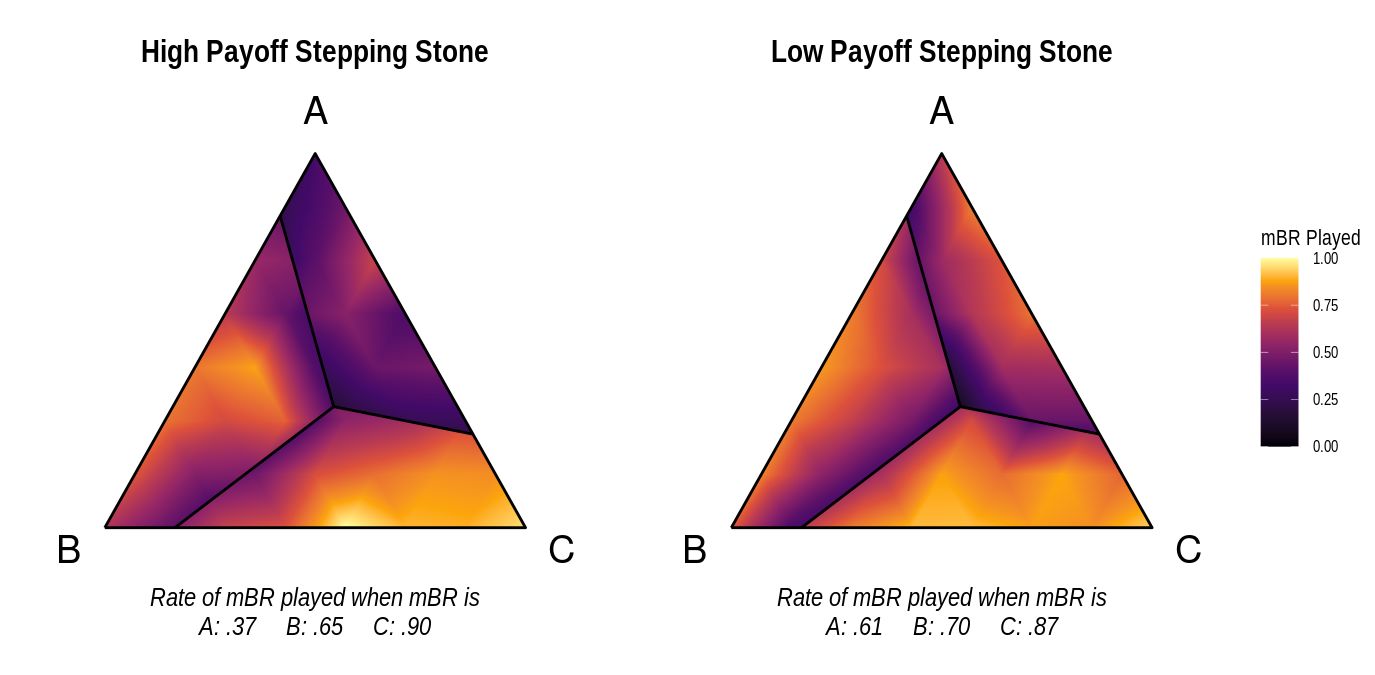
\includegraphics[width = \textwidth]{Images/Games23MBRPlot.png}
\end{figure}

I also examined whether the likelihood of a subject playing the myopic best response is influenced by the difference in expected payoff between the myopic best response and the next highest option. 
I found a significant positive relationship, with a logistic parameter estimate of 
$0.1287$ and a $p-$value $<2 \times 10^{-16}$. Therefore, I rejected hypothesis $4_0$ in favor of hypothesis $4_A$, suggesting that a larger difference in expected payoff leads to a higher probability of myopic best response play. This result in part explains why the mBR plots in Figures \ref{fig:Games23MBRPlot} and \ref{fig:GamesCIMBRPlot} are notably dark around the mBR boundaries.


\begin{figure}[h]
\captionsetup{justification=centering}
  \caption{Rate of Myopic Best Response Play by Strategy Profile Faced}
   \label{fig:GamesCIMBRPlot}
    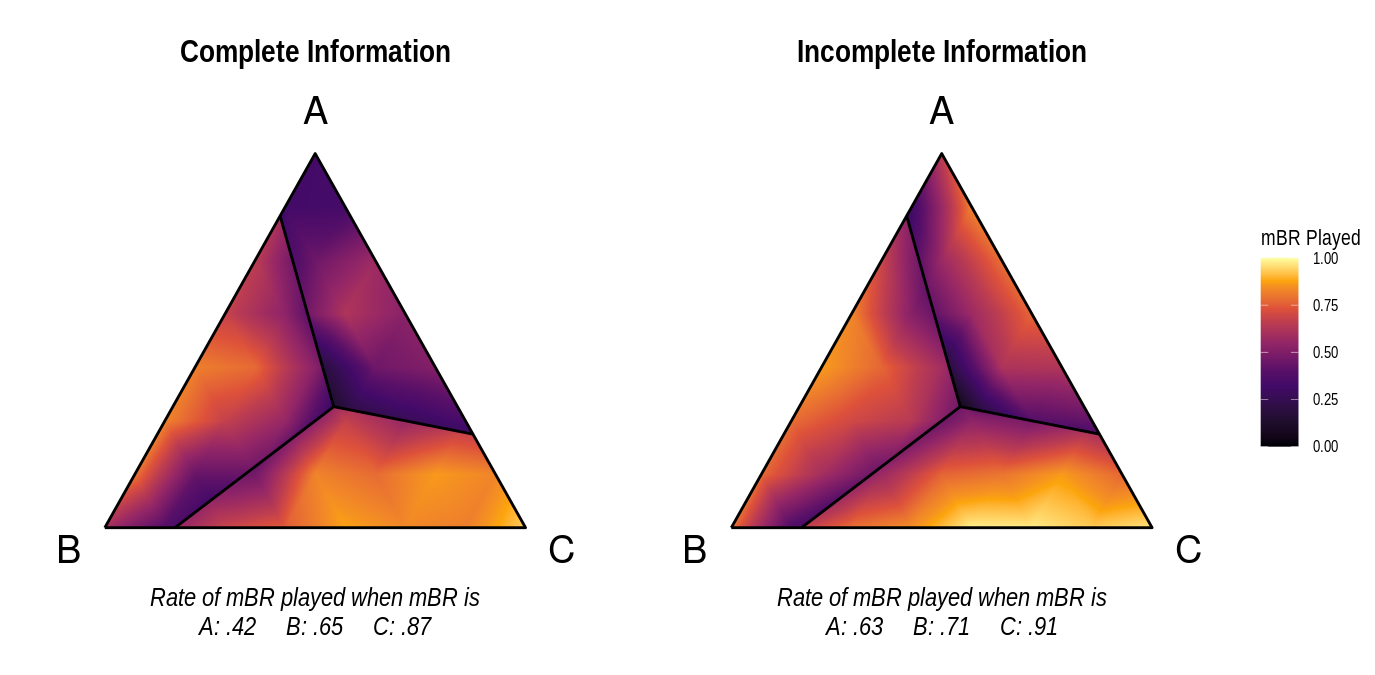
\includegraphics[width = \textwidth]{Images/GamesCIMBRPlot.png}
\end{figure}

I also examine Hypothesis 7, which explores whether the rate of deviations from the myopic best response, specifically when the myopic best response does not align with the Pareto efficient equilibrium, differs between games of \textit{complete information} and \textit{incomplete information}. To investigate this, I examine the interaction terms of myopic best response and \textit{incomplete information}. The point estimate of 0.7417 with a $p$-value = 0.000438 indicates that when information is incomplete and the myopic best response is $A$, subject are much more likely to play $A$ in games with \textit{incomplete information}. However, when the myopic best response is $B$, the combined point estimate is just 0.199872 and a resulting insignificant 1-sided $p$-value of 0.232. Although I can not claim that the subjects were statistically more likely to play $B$ when $B$ was the myopic best response when playing with \textit{incomplete information}, the combined results do provide significant support to hypothesis $7_A$. As such, I claim that the likelihood of deviating from the myopic best response is significantly higher in games with \textit{incomplete information} when the myopic best response does not correspond to the Pareto efficient equilibrium.


Related to my test of Hypothesis 4, I investigate whether the proportion of "mistakes" made by players choosing action $B$ in sessions playing Game 1 is significantly lower than $1/2$, indicating non-uniform distribution of mistakes. To test this, I employ a simple binomial test.

In the first 100 rounds, there were a total of 606 "mistakes" in sessions playing Game 1. Out of these mistakes, only 67 were players choosing action $B$. The binomial test yields compelling results. It allows me to reject Hypothesis $6_0$ in favor of $6_A$, as indicated by a $p$-value of less than $2.2e^{-16}$.




\section{Concluding Remarks}

In this paper I use the theoretical foundations of \cite{young1993evolution} and \cite{ellison2000basins} to define \textit{stepping stones}, a recurrent class which reduces the resistance from one recurrent class to another. I then design an experiment to test if injecting a stepping stone into a stag hunt game helps the group transition to the Pareto efficient equilibrium as theoretically predicted. I use a $3 \times 2$ treatment design varying the amount of information players receive about the game as well as the game they play and conducted 18 sessions in total, three for each treatment. 

The main results are as follows: First, I find that groups that played games with stepping stones were always able to make the transition to the risky, high payoff equilibrium and ended up playing the strategy associated with that equilibrium with the highest frequency. By contrast, groups without a stepping stone occasionally failed to make the transition. I also find that in games where the stepping stone payoff dominated the starting equilibrium, groups were more stable at and ended up playing the Pareto efficient equilibrium significantly more than when the starting equilibrium payoff dominated the stepping stone. 

Second, in examining the effect that information about other players\textquotesingle{} payoffs had on the game, I found that the groups who played with \textit{complete information} were more successful than groups with \textit{incomplete information} when playing the stag hunt game with no stepping stone. I attribute this to the common knowledge that a Pareto improvement exists. However, I find that this effect disappeared when a stepping stone was added to the game, presumably because the stepping stone offered easy to accomplish transitions at a low deviation cost. 

Finally, I examine how players made decisions in relation to their myopic best response.  examining myopic best response, the decision making mechanism behind adaptive play models. Recent experiments have found that subjects play their myopic best response 90-96\% of the time which provides good support for using the adaptive learning model in analyzing evolutionary games. In this experiment I find that subjects played their myopic best response 87-91\% of the time when their myopic best response corresponded with the Pareto efficient equilibrium which is in line with what's been observed in the literature.
I found several factors that influenced subjects propensity to deviate. Like \cite{lim2016experimental}, I find that players are more likely to deviate from myopic best response in the initial stages of the game and that players were sensitive to the difference in myopic payoffs. Specifically, players were less likely to play their myopic best response when the difference in myopic payoffs between that and an alternative strategy was lower. I also found that the largest factor in determining if a player would play their myopic best response is if their myopic best response corresponds to the payoff dominant equilibrium, adding support to the theory of \cite{harsanyi1988general} and results of \cite{jagau2022}. As such, combining the current data with a payoff-dependent mistakes model would give more powerful analysis.

I also adapted the stochastic strategy update probability used in experiments like \cite{hwang2018conventional} by first soliciting players decisions before the stochastic determination. This pseudo-strategy method allowed me to boost data collection and provided an interesting result. When subjects choices were not accepted in the previous round they were slightly but significantly less likely to deviate from myopic best response in the subsequent round. I attribute this to the increased salience that they could get stuck in an inefficient choice for multiple rounds. Further testing is required to see if this same effect impacts play when the stochastic determination is made prior to the player's decision. 


%--- Chapter 3 ----------------------------------------------------------------%
\chapter{Minimally Incomplete Sampling and Convergence of Adaptive Play in $2\times 2$ Games}

This chapter is co-authored with Anne van den Nouweland. I contributed to proving the main results and wrote the introduction. The proofs and results were written by both myself and Anne van den Nouweland who also provided editorial assistance throughout.

\section{Introduction}
With over 1000 citations, \cite{young1993evolution} is a seminal paper in the field of evolutionary game theory. In it, Young introduces a model of learning called adaptive play in which players best respond to a sampled history of play. Young proved that play will eventually converge to a convention, a self-enforcing pattern of play where the same Nash equilibrium is played in each period, if the sampling in the available history by the players is sufficiently incomplete. Through this backward looking best response behavior, Young offers an explanation for how order and norms can spontaneously evolve in populations.

In the process of adaptive play, occasionally players make mistakes and play an action that is not a best response. Such instances are called perturbations and allow the perturbed adaptive play process to escape a convention and travel to another one. The resistance of moving from one convention to another is measured by the number of mistakes that are necessary to move the process into the basin of attraction of the latter convention. The conventions that require the most mistakes to move from and/or the fewest to move to are most likely to be played in the long run. Such conventions are said to be stochastically stable. The theory of adaptive play, sometimes called adaptive learning or fictitious play with bounded memory, and its most celebrated result, identifying the 
stochastically stable patterns of play, have since been applied to a wide variety of games. We restrict the scope of our literature review here to games with finitely many strategies 
in which groups of players interact with each other on a random basis.\footnote{So, we do not, for example, consider games played on networks. For an introduction and references to the extensive  literature on such games, we refer to reader to \cite{WALLACE2015327}.
}

In his book \emph{Individual Strategy and Social Structure} (\cite{Young1998}),
 Young expanded upon the foundation he laid in \cite{young1993evolution}. He proved that in 
$2\times 2$ coordination games adaptive play eventually converges to a convention if the amount sampled ($s$) in the available memory ($m$) is sufficiently incomplete, where the criterion for "sufficiently" incomplete is slackened to $s/m \leq 1/2$ in \cite{Young1998} (from the more permissive restriction in \cite{young1993evolution}\footnote{The result in \cite{young1993evolution} that we are referring to is Theorem 1, which is formulated for a more general setting than only $2\times 2$ coordination games.}). 
%
Most recently, Proposition 6.4 of \cite{WALLACE2015327} simply states that in n-player coordination games "if s/m is sufficiently small, the [adaptive learning] process converges with probability one to a convention from any initial state". 
Although acknowledged by Young in his 1998 book, "We do not claim the bound on incompleteness $s/m \leq 1/2$ is the best possible", to our knowledge no one has found and proven what the best possible bound is. Consequently, follow-up work building upon this theory has retained the restrictive bound of $s/m \leq 1/2$. 

The literature we review applies adaptive learning to a variety of games with a focus on finding different criteria for stochastic stability. \cite{maruta1997relationship} and \cite{ellison2000basins} independently introduced the idea of global risk dominance,\footnote{The terminology "global risk dominance" was introduced in \cite{maruta1997relationship}.}  which indicates the existence of an action that risk dominates every other strategy in a game, and showed that the stochastic adaptive learning process of \cite{young1993evolution} selects the globally risk dominant strategy if there is one.

\cite{durieu2011adaptive} applied Young's adaptive play model to the concept of $p$-best response sets. 
The idea of $p$-dominant equilibrium, first introduced by \cite{morris1995p}, was adapted by \cite{tercieux2006p} to create the concept of $p$-best response sets.
A $p$-best response set is a cartesian product of strategies for each player such that when all players believe all other player(s) will play a strategy contributing to the $p$-best response set with at least probability $p$ then the best response(s) of all players are strategies contributing to the $p$-best response set.
A $p$-best response set with $p=1$ is therefore equivalent to the concept of a so-called curb set as introduced by \cite{basu1991strategy} and discussed in the context of adaptive play in Chapter 7 of \cite{Young1998}. 
A $p$-best response set is said to be minimal if it contains no proper subsets which are also $p$-best response sets.  \cite{durieu2011adaptive} show that in n-person games, if $p$ is sufficiently small then there is a unique minimal $p$-best response set and only the strategy profiles contained within the 
unique minimal $p$-best response set can be stochastically stable given perturbation rates are also sufficiently small.
Note that this method does not necessarily make as sharp a prediction as \cite{young1993evolution} since a $p$-best response set may contain multiple conventions of which not all are stochastically stable.

Breaking off from the canonical model, adaptive play has also been modified to fit a cognitive hierarchy framework \citep{saez1999clever, matros2003clever, khan2014cognitive}. This branch of theory allows for variability in the degree of sophistication through which players compute their best response, similar to level-k thinking as introduced by \cite{nagel1995unraveling}. In Young's model of adaptive play, agents are backwards looking and best respond to their sample of their opponents' play. \cite{saez1999clever} and \cite{matros2003clever} refer to these players as "not clever" and \cite{khan2014cognitive} refers to them as "level-1" individuals. One step higher on the cognitive scale are the "clever" and "level-2" individuals. These players sample their own history of play, compute their 
opponents' best responses to that, and then play their own best response to their opponents' predicted play. 
\cite{saez1999clever} and \cite{matros2003clever} cap the cognitive hierarchy at level-2 whereas \cite{khan2014cognitive} allows higher levels and moreover has even-leveled individuals sample their own history and odd-leveled individuals sample their opponents' history. 
\cite{saez1999clever} studies bargaining games, \cite{matros2003clever} studies generic two-player games, and \cite{khan2014cognitive} covers both of these. All three impose $s \leq m/2$\footnote{The authors allow for different roles in the game to have different sample sizes but impose the upper limit of $m/2$ for all samples.} and find that introducing "clever" agents can change which states are stochastically stable. \cite{matros2003clever} and \cite{khan2014cognitive} find that play with "clever" agents still converges to a minimal curb set.

\cite{jensen2005evolution} applies adaptive play to static $2$-player games of incomplete information. They allow for different types of players within the class of players for each role in the game, where  each type of player creates their own history. In each period, only the memories of the types who are selected to play are updated, and those of the other types remain unchanged. Players know the distribution of types in the other classes and sample for each type from the most recent $m$ periods in which that type played, and then weight their sample by the prevalence of each type and subsequently compute their best response. 
\cite{jensen2005evolution} examines in detail a $2\times 2$ game of chicken with incomplete information and leverages the condition $s<m/4$ (which they obtain by applying Theorem 1 in  \cite{young1993evolution})
to show that the basic learning process converges to a convention and that convention may be one which "lacks coordination" where not all types for the same player play the same strategy. Depending on the payoffs in the game, this "uncoordinated" convention can be stochastically stable. 

In our paper we show that \textit{any} degree of incomplete sampling is sufficient for the unperturbed adaptive play process to converge to an equilibrium in $2\times 2$ coordination games from any given history. In addition, we show that incomplete sampling is unnecessary in all but some $2 \times 2$ games. We also show that increasing the sample size beyond $s/m \leq 1/2$ may result in increased levels of resistance between conventions, that is to say, increasing the sample size may make conventions more stable. However, even though the resistance between conventions may change, we show that this change does not affect which convention(s) are stochastically stable when sampling is incomplete ($s<m$).

\section{Adaptive play in $2\times 2$ coordination games}

\subsection{$2\times 2$ coordination games}

Consider a $2\times 2$ game $G=(N;A_1,A_2;u_1, u_2)$ with player set $N=\{1,2\}$, actions sets $A_1=\{a_1,a_2\}$ and $A_2=\{b_1,b_2\}$, and payoff functions $u_i: A_1\times A_2 \rightarrow \bf{R}$ ($i=1,2$). The game $G$ is a coordination game if it has two pure-strategy Nash equilibria on a diagonal. Without loss of generality, we assume that $(a_1,b_1)$ and $(a_2,b_2)$ are Nash equilibria and we also assume that for player 1 either $u_1(a_1,b_1) > u_1(a_2,b_1)$ or $u_1(a_2,b_2) > u_1(a_1,b_2)$ and for player 2 either $u_2(a_1,b_1) > u_2(a_1,b_2)$ or $u_2(a_2,b_2) > u_2(a_2,b_1)$. These last two conditions rule out the possibility that one of the players has the same payoff from both their actions regardless of the action played by the other player, in which case the only distinction between a player's two actions is, from their own perspective, the names of the actions.

Because each player has only two actions in the game $G$, every mixed strategy $p_i$ of player $i\in \{1,2\}$ can be identified by the probability $p_i(s_i)$ with which player~$i$ plays one of their actions~$s_i$ (because that leaves probability $1-p_i(s_i)$ that player~$i$ plays their other action). 
%
Action $a_1$ is a best response by player~$1$ to a mixed strategy $p_2$ of player~$2$ if and only if 
$p_2(b_1) \geq \frac{u_1(a_2,b_2)-u_1(a_1,b_2)}{u_1(a_1,b_1)-u_1(a_1,b_2)-u_1(a_2,b_1)+u_1(a_2,b_2)}.$ Note that $\alpha_2 :=\frac{u_1(a_2,b_2)-u_1(a_1,b_2)}{u_1(a_1,b_1)-u_1(a_1,b_2)-u_1(a_2,b_1)+u_1(a_2,b_2)}\in [0,1]$ because $G$ is a coordination game with Nash equilibria $(a_1,b_1)$ and $(a_2,b_2)$, and either $u_1(a_1,b_1) > u_1(a_2,b_1)$ or $u_1(a_2,b_2) > u_1(a_1,b_2)$.\footnote{The only possible hick-up is that the denominator could equal 0, but that is ruled out when player~$1$ has two actions that differ to them in more than name only.}
%
Similarly, action $b_1$ is a best response by player~$2$ to a mixed strategy $p_1$ of player~$1$ if and only if 
$p_1(a_1) \geq \alpha_1 := \frac{u_2(a_2,b_2)-u_2(a_2,b_1)}{u_2(a_1,b_1)-u_2(a_2,b_1)-u_2(a_1,b_2)+u_2(a_2,b_2)} \in [0,1]$.


\subsection{Adaptive play in 2-player games}
 
We study adaptive play \citep{young1993evolution} with memory $m$ and sample size $1<k\leq m$ of the game~$G$, as explained below.\footnote{Throughout, we use $k$ for the sample size because we already use $s$ for strategies.} 

For each role (player position)~$i\in N$ in game~$G$, there is a class of players $C_i$ who can play that role. No player can play in more than one role ($C_1\cap C_2=\emptyset$). 
In each period $t$, a player is drawn from each class, and the two players that are drawn play the game $G$ -- each player~$i$ chooses an action $s_i(t)\in A_i$ from the actions available to them in their role. 
The action-tuple $s(t) = (s_1(t), s_2(t))$ is recorded and will be referred to as the play at time $t$. 
The history of plays up to and including time $t$ is the ordered vector $h(t) = (s(1), s(2), s(3), ..., s(t))$, and the history of the last $m$ plays, called a state, is the ordered vector $h(t|m) = (s(t-m+1), s(t-m+2), ..., s(t))$.

In period $t+1$, the player in role~$i$ draws a sample $R_i^{t+1}$ of size $k$ from the $m$ most recent plays $s_j(t-m+1), s_j(t-m+2), \ldots, s_j(t)$ by the players in role~$j\neq i$. 
Player~$i$ predicts that the players in role~$j$ play a mixed strategy $p_j(\cdot | R_i^{t+1})$ that is the frequency distribution of the actions in the sample drawn: $p_j(s_j | R_i^{t+1})$ equals the number of times that action $s_j$ occurs in the sample $R_i^{t+1}$ divided by $k$, for each $s_j\in A_j$. 
%
Player~$i$ then plays an action that is a best response to this predicted mixed strategy:  
$s_i(t+1)\in BR_i(R_i^{t+1}):=\arg\max \,\{ \sum_{s_j\in A_j} \left( p_j(s_j | R_i^{t+1})\cdot u_i(s_i,s_j) \right) \mid s_i\in A_i \} .$


\bigskip

The decision making process described above is called unperturbed adaptive play with memory size $m$ and sample size $k$. Through an adaptive play process, self-enforcing patterns of play, called conventions, can emerge.


\begin{definition}
A {\emph{convention}} is a state $h(t|m)$ that entirely consists of $m$ repetitions of the same Nash equilibrium $s^*$ of the game~$G$.
\end{definition}

When a convention is reached in which the Nash equilibrium $s^*$ is played, then the players can only sample the others playing their part of $s^*$ and thus all players have a best response to play their part of~$s^*$. That means that adaptive play predicts that the players can keep playing $s^*$ in all subsequent periods. If the Nash equilibrium $s^*$ is strict, then the best responses are unique and, without perturbations, the players will keep playing $s^*$ indefinitely. 

\section{Minimally incomplete sampling} 



In \cite{Young1998}, Young proved that in $2\times 2$ coordination games, unperturbed adaptive play will reach a convention as long as sampling is sufficiently incomplete. Incomplete sampling means that the players sample only a faction of the records in memory and in \cite{Young1998} the specific limit for sampling to be "sufficiently" incomplete is $k \leq \frac{m}{2}$, meaning that players sample at most half of all the records available in memory. 
We relax this bound substantially and show that in $2\times 2$ coordination games, {\emph {any} }degree of incomplete sampling is sufficient for a convention to eventually be reached.




%\justifying

Lemma~\ref{Lemma_1} will be used in the proof of Theorems~\ref{Theorem_1}, \ref{Theorem_2} and \ref{Theorem_3}.

\vskip12pt


%\noindent ********************************************************************


\begin{lemma}\label{Lemma_1} Let G be a 2$\times$2 coordination game and let $s^* = (s^*_1, s^*_2)$ be a (pure-strategy) Nash equilibrium of $G$. Consider unperturbed adaptive play with memory size $m$ and sample size $k\leq m$. Let $t > m$ be a period in which each player~$i\in\{1,2\}$ can play $s^*_i$ as a best response to their sampled history, so that there is a positive probability that the strategy-tuple $s^*$ is played in period~$t$. Then the convention of playing $s^*$ can be reached with positive probability.
\end{lemma}



\textbf{Proof of Lemma~\ref{Lemma_1}.} 

Using induction, we show that there exists a positive probability that $s^*$ is played in periods $t$ through $t+m-1$, so that the convention of playing $s^*$ is reached.

\textit{Base Step:} By assumption, the strategy-tuple $s^* = (s^*_1, s^*_2)$ is played with positive probability in period~$t$.



\textit{Inductive Step:} Let $\hat{t}\geq t$ and suppose that it has already been demonstrated that each player~$i\in\{1,2\}$ can play $s^*_i$ as a best response to their sampled history in period $\hat{t}$, so that there is a positive probability that the strategy-tuple $s^*$ is played in period~$\hat{t}$. It will be shown that there is a positive probability that $s^*$ is played in period~$\hat{t}+1$ as part of adaptive play. 

\vskip6pt

For each player $i\in \{1,2\}$, let $R_i^{\hat{t}}$ be a sampled history of player~$i$ in period~$\hat{t}$ such that $s^*_i\in BR_i(R_i^{\hat{t}})$, and let $s_i(\hat{t})=s_i^*$. Then there is a positive probability that each player~$i$ draws a sample $R_i^{\hat{t}+1}$ that is obtained by replacing one of the records in $R_i^{\hat{t}}$ with $s_j(\hat{t})=s_j^*$ ($j\neq i$). If the replaced record is equal to $s_j^*$, then this does not change the frequency of $s_j^*$ in~$i$'s sample, and if the replaced record is not equal to $s_j^*$, then this increases the frequency of $s_j^*$ in~$i$'s sample. 
If $s^* =(a_1,b_1)$, then $p_j(s_j^* | R_i^{\hat{t}+1})\geq p_j(s_j^* | R_i^{\hat{t}})\geq \alpha_j,$ where the last step holds because $s^*_i\in BR_i(R_i^{\hat{t}})$. 
Similarly, if $s^* =(a_2,b_2)$, then $p_j(s_j^* | R_i^{\hat{t}+1})\geq p_j(s_j^* | R_i^{\hat{t}})\geq 1-\alpha_j.$ 
In both cases,  it follows that $s^*_i\in BR_i(R_i^{\hat{t}+1})$.

Therefore, there is a positive probability that $s^*$ is played in period~$\hat{t}+1$ as part of adaptive play. 

\medskip
\textit{Conclusion:} Using the inductive step $m-1$ times, it has thus been shown that there exists a positive probability that $s^*$ is played in periods $t$ through $t+m-1$, so that the convention of playing $s^*$ is reached.
$\blacksquare$



%\vskip18pt
\bigskip

Lemma~\ref{Lemma_1} exploits the fact that in a $2\times 2$ game, when player~$i$'s Nash equilibrium action $s_i^*$ is a best response to the other player~$j$'s mixed strategy, and subsequently, the probability that player~$j$ plays $s_j^*$ (weakly) increases, then $s_i^*$ is still a best response by player~$i$. 
Loosely speaking, it seems fairly intuitive that a when the other player plays their Nash equilibrium action with larger probability, this will increase a player's incentive to play their best response to that action. However, the following example demonstrates that this intuition does not extend to larger games. 

\begin{example}\label{Example_lemma_1} Consider the $3\times 3$ coordination game in Figure~\ref{fig:game4}
%\centering
\begin{figure}[h]
\caption{Example~\ref{Example_lemma_1} Game}
\label{fig:game4}
$$\begin{tabular}{cc|c|c|c|}
      & \multicolumn{1}{c}{} & \multicolumn{2}{c}{Player 2} & \multicolumn{1}{c}{}\\
      & \multicolumn{1}{c}{} & \multicolumn{1}{c}{$b_1$}  & \multicolumn{1}{c}{$b_2$} & \multicolumn{1}{c}{$b_3$}\\\cline{3-5}
      \multirow{3}*{Player 1}  & $a_1$ & ${1,1}$ & $0,0$ & $0,0$ \\\cline{3-5}
      & $a_2$ & $0,0$ & ${2,2}$ & $-3,-3$ \\\cline{3-5}
       & $a_3$ & $0,0$ & $-3,-3$ & ${2,2}$ \\\cline{3-5}
    \end{tabular}
$$
\end{figure}
\medskip
\noindent

Suppose that $t > m \geq k=2$, $R_1^t = \{b_3, b_2\}$ and $R_2^t = \{a_2, a_3\}$. Given the distribution of the sampled actions of player~2 in~$R_1^t$, player 1 has an expected payoff of $0$ if they play $a_1$, $-\frac{1}{2}$ if they play $a_2$, and $-\frac{1}{2}$ if they play $a_3$, so that $BR_1(R_1^t)=\{a_1\}$. Given the distribution of the sampled actions of player~1 in~$R_2^t$, player~2 has an expected payoff of $0$ if they play $b_1$, $-\frac{1}{2}$ if they play $b_2$, and $-\frac{1}{2}$ if they play $b_3$, so that $BR_2(R_2^t)=\{b_1\}$. 
Thus, the strict Nash equilibrium $(a_1, b_1)$ is played with positive probability period~$t$.

Let $s(t) = (a_1, b_1)$ and suppose that in period $t+1$ both players sample the record played in period $t$. 
Assuming that player~1 draws the record $s_2(t)=b_1$ instead of one of the two records $b_2$ or $b_3$ drawn in $R_1^t$, there are two possibilities, namely $R_1^{t+1}=\{b_1,b_2\}$ and $R_1^{t+1}=\{b_1,b_3\}$. Because $BR_1(\{b_1,b_2\})=\{a_2\}$ and $BR_1(\{b_1,b_3\})=\{a_3\}$, it is no longer a best response for player~1 to play~$b_1$ if they replace any of the records that they sampled at time~$t$ with the record of player~2 playing $b_1$ at time~$t$. 
%
It is thus possible that adaptive play leads players away from the strict Nash equilibrium $(a_1,b_1)$ after a period in which that strategy profile is played by the two players. 
\end{example}



While Example~\ref{Example_lemma_1} demonstrates that the proof that we provided of Lemma~\ref{Lemma_1} is not valid for coordination games in which players have more than 2 actions, the following example demonstrates that when sampling is complete ($k=m$), the statement of the lemma is not necessarily true for such games.  

\begin{example}\label{Example2_lemma_1} 
Consider the game in Example~\ref{Example_lemma_1} and let $k = m = 2$. Consider a period 
$t > 2$ such that  $h(t\mid m) = \big((a_2, b_3), (a_3, b_2)\big)$. Because sampling is complete, $R_1^{t+1} = \{b_2, b_3\}$ and $R_2^{t+1} = \{a_2, a_3\}$. 
Because $BR_1(\{b_2, b_3\})=\{a_1\}$ and $BR_2(\{a_2, a_3\})=\{b_1\}$, necessarily $s(t+1) = (a_1, b_1)$. 
%
Thus, $h(t+1\mid m) = \big((a_3, b_2), (a_1, b_1)\big)$, $R_1^{t+2} = \{b_1, b_2\}$, and $R_2^{t+2} = \{a_1, a_3\}$. 
Therefore, $BR_1(R_1^{t+2})=\{a_2\}$ and $BR_2(R_2^{t+2})=\{b_3\}$, and necessarily $s(t+2) = (a_2, b_3)$. 
%
It follows that in period $t+3$, the players see the history $h(t+2\mid m) = \big((a_1,b_1),(a_2, b_3)\big)$, 
so that $R_1^{t+3} = \{b_1, b_3\}$ and $R_2^{t+3} = \{a_1, a_2\}$, and the players' best responses are $BR_1(R_1^{t+3})=\{a_3\}$ and $BR_2(R_1^{t+3})=\{b_2\}$. 
%
After playing $s(t+3) = (a_3, b_2)$, the history of the last $m$ plays is $h(t+3\mid m) = \big((a_2, b_3), (a_3, b_2)\big)$ and the adaptive play process has thus returned to the same state it was in during period $t$. 

We have demonstrated that adaptive play with memory size $2$ and complete sampling (sample size 2) will keep cycling from $(a_2, b_3)$ to $(a_3, b_2)$ to $(a_1, b_1)$, to $(a_2, b_3)$, to  $(a_3, b_2)$, and so on.  
%
Thus, although the strict Nash equilibrium: $(a_1, b_1)$ is played every third period as part of this sequence, the process never reaches the convention of playing $(a_1, b_1)$. 
\end{example}



\begin{theorem}\label{Theorem_1}
Let G be a 2$\times$2 coordination game with Nash equilibria $(a_1,b_1)$ and $(a_2,b_2)$,  
in which at least one of the two Nash equilibria is strict (i.e., either $u_1(a_1,b_1) > u_1(a_2,b_1)$ and $u_2(a_1,b_1) > u_2(a_1,b_2)$, or $u_1(a_2,b_2) > u_1(a_1,b_2)$ and $u_2(a_2,b_2) > u_2(a_2,b_1)$). 
%
From any initial state, unperturbed adaptive play with memory size $m$ and sample size $k < m$ converges with probability one to a convention corresponding to a strict Nash equilibrium and locks in.
\end{theorem}


\textbf{Proof of Theorem~\ref{Theorem_1}.}
In light of Lemma~\ref{Lemma_1}, it suffices to demonstrate that there exists a period $t > m$ in which a strict Nash equilibrium $s^*=(s_1^*,s_2^*)$ is played with positive probability, because then the convention of playing $s^*$ can be reached with positive probability, and once that convention is reached, the players will keep playing $s^*$ indefinitely.

Without loss of generality, assume that the Nash equilibrium $(a_1,b_1)$ is strict. 
%
Consider unperturbed adaptive play with memory size $m$ and sample size $k < m$ starting from an arbitrary initial state. Consider an arbitrary period $t>m$ and the history $h(t) = (s(1), s(2), s(3), ..., s(t))$ of plays up to and including time $t$. 
%
We distinguish three cases.

{\bf Case 1. } In period $t+1$ it is possible for the players to draw samples $R_i^{t+1}$, $i=1,2$, such that $a_1\in BR_1(R_1^{t+1})$ and $b_1\in BR_2(R_2^{t+1})$. Then there is a positive probability that $s(t+1)=(a_1,b_1)$. 

{\bf Case 2. } In period $t+1$ it is possible for the players to draw samples $R_i^{t+1}$, $i=1,2$, such that $a_2\in BR_1(R_1^{t+1})$ and $b_2\in BR_2(R_2^{t+1})$. There is a positive probability that $s(t+1)=(a_2,b_2)$. If the Nash equilibrium $(a_2,b_2)$ is strict, then we have reached a period in which the players play a strict Nash equilibrium.  
%

If the Nash equilibrium $(a_2,b_2)$ is not strict, then $u_1(a_2,b_2) = u_1(a_1,b_2)$ or $u_2(a_2,b_2) = u_2(a_2,b_1)$ (or both). Assume, without loss of generality, that $u_1(a_2,b_2) = u_1(a_1,b_2)$ (and $u_2(a_2,b_2) \geq u_2(a_2,b_1)$). Then $BR_1(R_1^{t+1})=\{a_1,a_2\}$ and thus $a_1\in BR_1(R_1^{t+1})$. Thus, $s(t+1)=(a_1,b_2)$ is played with positive probability in the adaptive play process. For the next $k-1$ periods, regardless of the actions that player 2 plays and the samples that player 1 draws, player 1 can keep playing $s_1(\hat{t})=a_1$, $\hat{t}=t+2, \ldots, t+k$, as a best response. Then in period $t+k+1$, player 2 can draw a sample $R_2^{t+k+1}$ from player 1's actions that consists of $k$ instances of player 1 playing $a_1$, so that $b_1\in BR_2(R_2^{t+k+1})$. Thus, there is a positive probability that $s(t+k+1)=(a_1,b_1)$. 

{\bf Case 3.} If in period $t+1$ it is not possible for the players to draw samples $R_i^{t+1}$, $i=1,2$, such that $s_i\in BR_i(R_i^{t+1})$ for $i=1,2$ and $(s_1,s_2)$ is a Nash equilibrium of $G$, then, without loss of generality, assume that $BR_1(R_1^{t+1})=\{a_1\}$ for all samples that player 1 can draw, and $BR_2(R_2^{t+1})=\{b_2\}$ for all samples that player 2 can draw, so that $s(t+1)=(a_1,b_2)$. 
%

This implies that in $h(t\mid m)$ player 2 played $b_2$ at most $\beta_2$ times, where $\beta_2$ is the largest number in $\{ 0,1,\ldots, k-1\}$ that is strictly lower than $(1-\alpha_2)\times k$.\footnote{We remind the reader that $\alpha_2$ is the probability such that action $a_1$ is a best response by player~$1$ to a mixed strategy $p_2$ of player~$2$ if and only if 
$p_2(b_1) \geq \alpha_2$. Also, because $(a_1,b_1)$ is a strict Nash equilibrium, $\alpha_2 < 1$, so that $(1-\alpha_2)\times k > 0$.}
Similarly, in $h(t\mid m)$ player 1 played $a_1$ at most $\beta_1$ times, where $\beta_1$ is the largest number in $\{ 0, 1,\ldots, k-1\}$ that is strictly lower than $\alpha_1\times k$.\footnote{We remind the reader that $\alpha_1$ is the probability such that action $b_1$ is a best response by player~$2$ to a mixed strategy $p_1$ of player~$1$ if and only if 
$p_1(a_1) \geq \alpha_1$. Note that $\alpha_1 > 0$, because otherwise $b_1\in BR_2(R_2^{t+1})$ regardless of the sample that player 2 draws.} 
However, $s(t+1)=(a_1,b_2)$, so that the number of times that player 1 (resp. 2) plays action $a_1$ (resp. $b_2$) in $h(t+1\mid m)$ is either equal to that in $h(t\mid m)$ (in case $s_1(t-m+1)=a_1$, resp. $s_2(t-m+1)=b_2$) or one higher. 
As long as these numbers do not exceed $\beta_1$, resp. $\beta_2$, the players will keep playing $s(\hat{t})=(a_1,b_2)$ in periods $\hat{t} \geq t+2$. This clearly cannot persist because after $m$ periods the players would only have plays $(a_1,b_2)$ in recent memory. 
%

Let $\hat{t}\geq t+1$ be the first period in which either player 1 played $a_1$ more than $\beta_1$ times in $h(\hat{t}\mid m)$ or player 2 played $b_2$ more than $\beta_2$ times in $h(\hat{t}\mid m)$ (or both). %
Without loss of generality, assume that player 1 played $\beta_1$ instances of $a_1$ in $h(\hat{t}-1\mid m)$ and $\beta_1+1$ instances of $a_1$ in $h(\hat{t}\mid m)$. 
%Thus, $s_1(\hat{t})=a_1$ and $s_1(\hat{t}-m)=a_2$. 
%
Then in period $\hat{t}+1$, player 2 can draw a sample $R_2^{\hat{t}+1}$ that contains $\beta_1+1$ instances of player 1 playing $a_1$, and play $s_2(\hat{t}+1)=b_1\in BR_2(R_2^{\hat{t}+1})$. 
%
Also, player 2 played at most $\beta_2$ instances of $b_2$ in $h(\hat{t}-1\mid m)$), and thus at most $\beta_2+1$ instances of $b_2$ in $h(\hat{t}\mid m)$). Thus, because $k<m$, in period $\hat{t}+1$, player 1 can draw a sample $R_1^{\hat{t}+1}$ that contains no more than $\beta_2$ instances of player 2 playing $b_2$, and play $s_1(\hat{t}+1)=a_1\in BR_1(R_1^{\hat{t}+1})$. 
%
Thus, there is a positive probability that $s(\hat{t}+1)=(a_1,b_1)$. 

{\bf Conclusion.} The three cases we considered are exhaustive and thus we have shown that, starting  from any period $t>m$ and with any history of play at that time, we can find a period in which there is a positive probability that the players play a strict Nash equilibrium in the adaptive play process with sample size $k<m$. Lemma~\ref{Lemma_1} then establishes that the convention of playing that strict Nash equilibrium can be reached with positive probability, and then the process is locked in.
$\blacksquare$

\medskip
Note that in the proof of Theorem~\ref{Theorem_1}, there is only one instance in which we use that sampling is incomplete ($k<m$), and that is in Case 3, where we need it to guarantee that it cannot be the case that the adaptive play process can get "stuck" in a situation where both players mis-coordinate in every period, oscillating between $(a_1,b_2)$ and $(a_2,b_1)$ and necessarily switching actions in exactly the same periods. 
%
If the game and sample sizes are such that this cannot happen anyway, then we do not need sampling to be incomplete at all, and we can have $k=m$. 
We use the notation $\lceil\cdot\rceil$ to denote the rounding up of any real number to the smallest natural number that is at least as large.\footnote{So, if $n$ is a natural number itself, then $\lceil n\rceil=n$. Also, we include $0$ in the set of natural numbers.}





\begin{theorem}\label{Theorem_2}
Let G be a 2$\times$2 coordination game with Nash equilibria $(a_1,b_1)$ and $(a_2,b_2)$,  
in which at least one of the two Nash equilibria is strict (i.e., either $u_1(a_1,b_1) > u_1(a_2,b_1)$ and $u_2(a_1,b_1) > u_2(a_1,b_2)$, or $u_1(a_2,b_2) > u_1(a_1,b_2)$ and $u_2(a_2,b_2) > u_2(a_2,b_1)$)  
%
and such that $\alpha_1\neq 1-\alpha_2$.\footnote{Thus, the smallest probability for player~1 to play $a_1$ such that action $b_1$ is a best response by player~$2$ is not equal to the smallest probability for player~2 to play $b_2$ such that action $a_2$ is a best response by player~$1$.} 
%
Let the sample size $k$ be such that $\lceil\alpha_1\times k\rceil \neq \lceil (1-\alpha_2)\times k\rceil$ or $\lceil\alpha_2\times k\rceil \neq \lceil (1-\alpha_1)\times k\rceil$.\footnote{Note that if the game $G$ is such that $\alpha_1$ and $1-\alpha_2$ are close, then this will require a large sample size.}\textsuperscript{,}\footnote{$\lceil\alpha_1\times k\rceil \neq \lceil (1-\alpha_2)\times k\rceil$ does not necessarily imply $\lceil\alpha_2\times k\rceil \neq \lceil (1-\alpha_1)\times k\rceil$. An example of this can be found in Example~\ref{Example_Theorem_4b}.}
From any initial state, unperturbed adaptive play with memory size $m$ and sample size $k \leq m$ converges with probability one to a convention corresponding to a strict Nash equilibrium and locks in.
\end{theorem}

\textbf{Proof of Theorem~\ref{Theorem_2}.}
If $k<m$, then Theorem~\ref{Theorem_1} applies. So, suppose that $k=m$, i.e, sampling is complete in the sense that players see \emph{all} of the past $m$ records.

Consider an adaptive play process with $k=m$. If in some period $t>m$ the players coordinate, i.e., $s(t)=(a_1,b_1)$ or $s(t)=(a_2,b_2)$, then we can apply cases 1 or 2 in the proof of Theorem~\ref{Theorem_1} to establish that there is a positive probability that the players play a strict Nash equilibrium (note that these cases do not depend on $k < m$). 
Lemma~\ref{Lemma_1} then establishes that the convention of playing that strict Nash equilibrium can be reached with positive probability, and then the process is locked in.

Thus, it remains to consider the possibility that the players mis-coordinate in all periods, i.e., $s(t)\in \{(a_1,b_2),(a_2,b_1)\}$ for all $t$. We will demonstrate that this cannot happen because one of $\lceil\alpha_1\times k\rceil \neq \lceil (1-\alpha_2)\times k\rceil$ or $\lceil\alpha_2\times k\rceil \neq \lceil (1-\alpha_1)\times k\rceil$ implies that an adaptive play process with $k=m$ cannot result in string of mis-coordinated plays $s(1),s(2), \ldots $ with $s(t)\in \{(a_1,b_2),(a_2,b_1)\}$ for all $t$. 
%
Without loss of generality assume $\lceil \alpha_1\times m\rceil \neq\lceil (1-\alpha_2)\times m\rceil$. If, in some period $t>m$,\footnote{We consider only periods $t>m$ to ensure that the players have $m$ periods' plays available in memory.} the players observe a history of play that consists of a string of $m$ instances of $(a_1,b_2)$ having been played in the previous $m$ periods, player~2's unique best response is to play~$b_1$ in the next period or player~1's unique best response is to play~$a_2$ in the next period.\footnote{This uses $\lceil \alpha_1\times m\rceil \neq\lceil (1-\alpha_2)\times m\rceil$, which implies that it cannot be the case that player 1 can best respond by playing~$a_1$ \emph{and} player 2 can best respond by playing~$b_2$ after both observe $m$ instances of $(a_1,b_2)$ having been played.} 
%
Thus, any string of mis-coordinated plays that contains a string of more than $m$ subsequent plays of $(a_1,b_2)$ cannot be the result of an adaptive play process. 
%
Similarly, any string of mis-coordinated plays that contains a string of more than $m$ subsequent plays of $(a_2,b_1)$ cannot be the result of an adaptive play process. 
%
We conclude that if the players mis-coordinate in all periods, and they follow an adaptive play process, then the process needs to switch repeatedly between playing $(a_1,b_2)$ and $(a_2,b_1)$. 

For player 1 to switch to playing $a_2$, they need to observe $\lceil (1-\alpha_2)\times m\rceil$ instances of player~2 playing $b_2$, and for player 2 to switch to playing $b_1$, they need to observe $\lceil \alpha_1\times m\rceil$ instances of player~1 playing $a_1$.
%
However, in all periods $t>m$, because $k=m$, player~1 samples as many records of player~2 playing $b_2$ as player~2 samples records of player~1 playing $a_1$. 
Thus, $\lceil \alpha_1\times m\rceil \neq\lceil (1-\alpha_2)\times m\rceil$ implies that the players will not switch from playing $(a_1,b_2)$ to playing $(a_2,b_1)$ in the same period when they follow an adaptive play process.    
%
$\blacksquare$

\section{Perturbed adaptive play in $2 \times 2$ games}

Now consider the adaptive play process as modeled in Section 2 but where players have a small probability of playing an action that is not their best response. Specifically, in every round players now play a strategy at random with probability $\varepsilon$ and with probability $1-\varepsilon$ they play a best response to their drawn sample, $R_i^{t}$. As such, an action that is not in the set of possible best responses to samples drawn from the memory can be played with probability $\varepsilon/2$.\footnote{The $1/2$ comes from the fact that each player has two actions, each of which they choose with equal probability when they
play an action at random.} We shall refer to such actions as \textit{mistakes}. This process is called perturbed adaptive play. Allowing for mistakes makes transitions possible between conventions, even those in which a strict Nash equilibrium is played. Continuing with the setup established in Section 2 where $(a_1, b_1)$ and $(a_2, b_2)$ are Nash equilibria, denote by $h_i$ the convention corresponding to $(a_i, b_i)$, i.e., the state that consists of $m$
repetitions of $(a_i, b_i)$.
Now consider the transition from $h_i$ to $h_j$. Let the resistance, denoted $r_{i,j}^{k,m}$, be the minimum number of mistakes necessary to make the transition from $h_i$ to $h_j$ in the perturbed adaptive play process.
\cite{Young1998} shows that the resistance between conventions is independent of $m$ when $k \leq m/2$. Specifically, the resistance of moving from $h_2$ to $h_1$ equals $\min\big(\lceil \alpha_1 \times k \rceil,\lceil \alpha_2 \times k \rceil\big)$ and the resistance of moving from $h_1$ to $h_2$ equals $\min\big(\lceil (1-\alpha_1) \times k \rceil,\lceil (1-\alpha_2) \times  k \rceil\big)$. However, we demonstrate below that when sampling is less incomplete ($k > m/2$), the resistances may be larger and depend on $m$.


\begin{theorem}\label{Theorem_3}
Let G be a 2$\times$2 coordination game with Nash equilibria $(a_1,b_1)$ and $(a_2,b_2)$. 
Consider unperturbed adaptive play with memory size $m$ and sample size $k\leq m$. 
The resistance of moving from $h_2$ to $h_1$ equals $r_{2,1}^{k,m} = \min\big(\lceil \alpha_1 \times k \rceil,\lceil \alpha_2 \times k \rceil\big)+\max\big(\lceil\alpha_1\times k\rceil+\lceil \alpha_2 \times k \rceil-m,0\big)$ and the resistance of moving from $h_1$ to $h_2$ equals $r^{k,m}_{1,2}=\min\big(\lceil (1-\alpha_1) \times k \rceil, \lceil (1-\alpha_2) \times  k \rceil\big)+\max\big(\lceil (1-\alpha_1) \times k \rceil+\lceil (1-\alpha_2) \times k \rceil-m,0\big)$. 
\end{theorem}


\textbf{Proof of Theorem~\ref{Theorem_3}.} 
We compute the resistance $r_{2,1}^{k,m}$. Similarly to Case 2 of the proof of Theorem~\ref{Theorem_1}, we derive that no mistakes are necessary to move from $h_2$ to $h_1$ if equilibrium $(a_2,b_2)$ is not strict. In that case, either $\alpha_1=0$ or $\alpha_2=0$ or both hold and the expression for $r_{2,1}^{k,m}$ in the statement of the theorem indeed produces a resistance equal to 0.  

So assume that equilibrium $(a_2,b_2)$ is strict and let $t$ be a period such that $h(t|m) = h_2$, i.e., the system is in convention $h_2$. 
Because $(a_2,b_2)$ is strict, $(a_2,b_2)$ will continue to be played if the players do not make any mistakes. To reach convention $h_1$, it is necessary to reach a period in which both $a_1$ and $b_1$ can be played as best responses to samples drawn by the players.\footnote{Note that this is a property that is satisfied by convention $h_1$.} 
Reaching a period in which both $a_1$ and $b_1$ can be played as best responses to samples drawn by the players is also a sufficient condition for the process to reach convention $h_1$ without further mistakes (see Lemma~\ref{Lemma_1}). 
%
Thus, starting from convention $h_2$, we need to determine the minimum number of mistakes (which will be positive) necessary to build a length-$m$ history of play from which both players can draw samples of size $k$ such that $a_1$ and $b_1$ are best responses. 
For this condition to be met in some period $T$, player~1 must have played $a_1$ at least $\lceil \alpha_1 \times k \rceil$ times and player~2 must have played $b_1$ at least $\lceil \alpha_2 \times k \rceil$ times in periods $T-m$ through $T-1$. 
%
Clearly, this can be accomplished by having player~1 make a mistake and play~$a_1$ a total of $\lceil \alpha_1 \times k \rceil$ times \emph{and} having player~2 make a mistake and play~$b_1$ a total of $\lceil \alpha_2 \times k \rceil$ times in $\max\big(\lceil \alpha_1 \times k \rceil,\lceil \alpha_2 \times k \rceil\big)$ consecutive periods. 
This gives an upper bound of $\lceil \alpha_1 \times k \rceil + \lceil \alpha_2 \times k \rceil$ for $r_{2,1}^{k,m}$.
%

The number of mistakes can be lowered by decreasing the number of periods in which both players make a mistake, so that players can sample each other's mistakes and potentially play $a_1$ and/or $b_1$ as best responses. 
 
At the extreme, when sample sizes are sufficiently incomplete so that players can keep sampling mistakes long enough, it suffices for one player to make enough mistakes to make their action in $(a_1,b_1)$ a best response by the other player, and we obtain the lower bound $\min\big(\lceil \alpha_1 \times k \rceil,\lceil \alpha_2 \times k \rceil\big)$ for $r_{2,1}^{k,m}$. 
We consider this case first. 

{\bf Case 1.} $\lceil \alpha_1 \times k \rceil + \lceil \alpha_2 \times k \rceil \leq m$.\footnote{In this case, derivations are similar to those in \cite{Young1998}.} 
%

Starting in period $t+1$, suppose player~1 makes $\lceil \alpha_1 \times k \rceil$ consecutive mistakes and plays $a_1$ in periods $t+1, \dots, t+ \lceil \alpha_1 \times k \rceil$. During each of these periods, player~2 can sample no more than $\lceil \alpha_1 \times k \rceil - 1$ instances of player~1 playing $a_1$ and can only play $b_2$ as a best response.

Because $\lceil \alpha_1 \times k \rceil + \lceil \alpha_2 \times k \rceil \leq m$, in each of the periods $t+\lceil \alpha_1 \times k \rceil + 1$ through $t + \lceil \alpha_1 \times k \rceil + \lceil \alpha_2 \times k \rceil$, player~2 can sample all $ \lceil \alpha_1 \times k \rceil $ instances of $a_1$ that player~1 played in periods $t+1$ to $t+\lceil \alpha_1 \times k \rceil$ and play $b_1$ as a best response. In these periods, player~1 can sample no more than $\lceil \alpha_2 \times k \rceil - 1$ plays of $b_1$ and can only play $a_2$ as a best response.

\begin{table}[h]
\caption{Case 1 Example Transition}
\label{tab:case1exampletransition} 
\centering
\resizebox{\linewidth}{!}{%
\begin{tabular}{|c|*{11}{c|}}
\hline
& \multicolumn{11}{|c|}{Play} \\
\hline
Period & $t-m+1$ & $\ldots$ & $t$ & $t+1$ & $\ldots$ & $t+\lceil\alpha_1\times k\rceil$ & $t+\lceil\alpha_1\times k\rceil+1$ & $\ldots$ & $t+\lceil\alpha_1\times k\rceil+\lceil\alpha_2\times k\rceil$ & $t+\lceil\alpha_1\times k\rceil+\lceil\alpha_2\times k\rceil+1$ & $\ldots$ \\
\hline
Player 1 & \textcolor{blue}{$a_2$} & \textcolor{blue}{$a_2$} & \textcolor{blue}{$a_2$} & \textcolor{red}{$a_1$} & \textcolor{red}{$a_1$} & \textcolor{red}{$a_1$} & \textcolor{blue}{$a_2$} & \textcolor{blue}{$a_2$} & \textcolor{blue}{$a_2$} & \textcolor{blue}{$a_1$} & \textcolor{blue}{$a_1$} \\
\hline
Player 2 & \textcolor{blue}{$b_2$} & \textcolor{blue}{$b_2$} & \textcolor{blue}{$b_2$} & \textcolor{blue}{$b_2$} & \textcolor{blue}{$b_2$} & \textcolor{blue}{$b_2$} & \textcolor{blue}{$b_1$} & \textcolor{blue}{$b_1$} & \textcolor{blue}{$b_1$} & \textcolor{blue}{$b_1$} & \textcolor{blue}{$b_1$} \\
\hline
\end{tabular}%
}
\small
The color red denotes actions which necessarily are mistakes. Actions colored blue can be played as a best response.
\end{table}


Because $\lceil \alpha_1 \times k \rceil + \lceil \alpha_2 \times k \rceil \leq m$, in period $t + \lceil \alpha_1 \times k \rceil + \lceil \alpha_2 \times k \rceil + 1$ it is possible for player~2 to sample all $\lceil \alpha_1 \times k \rceil$ player~1's plays of $a_1$ in periods $t + 1$ through $t + \lceil \alpha_1 \times k \rceil$, while player~1 samples all $\lceil \alpha_2 \times k \rceil $ player~2's plays of $b_1$ in periods $t+\lceil \alpha_1 \times k \rceil + 1$ through $t + \lceil \alpha_1 \times k \rceil + \lceil \alpha_2 \times k \rceil$. Thus, both $a_1$ and $b_1$ can be played as best responses by the players in period $t + \lceil \alpha_1 \times k \rceil + \lceil \alpha_2 \times k \rceil + 1$ and the process can reach convention $h_1$ without further mistakes (see Lemma~\ref{Lemma_1}). 

The  process we just described reaches convention $h_1$ from convention $h_2$ with exactly $\lceil \alpha_1 \times k \rceil$ mistakes by starting in period $t+1$ with player~1 making $\lceil \alpha_1 \times k \rceil$ consecutive mistakes and playing $a_1$ in periods $t+1, \dots, t+ \lceil \alpha_1 \times k \rceil$. If instead we start in period $t+1$ with player~2 making $\lceil \alpha_2 \times k \rceil$ consecutive mistakes and playing $b_1$ in periods $t+1, \dots, t+ \lceil \alpha_2 \times k \rceil$, we obtain a process that reaches convention $h_1$ from convention $h_2$ with exactly $\lceil \alpha_2 \times k \rceil$ mistakes. 

Because either player~1 must have played $a_1$ at least $\lceil \alpha_1 \times k \rceil$ times to allow player~2 to play $b_1$ as a best response, or player~2 must have played $b_1$ at least $\lceil \alpha_2 \times k \rceil$ times to allow player~1 to play $a_1$ as a best response, the minimum number of mistakes necessary to reach convention $h_1$ from convention $h_2$ equals $\min\big(\lceil \alpha_1 \times k \rceil,\lceil \alpha_2 \times k \rceil\big)$. Since (at least) one of the two processes we described reaches convention $h_1$ from convention $h_2$ with exactly $\min\big(\lceil \alpha_1 \times k \rceil,\lceil \alpha_2 \times k \rceil\big)$ mistakes, we have demonstrated that 
$r_{2,1}^{k,m} =  \min\big(\lceil \alpha_1 \times k \rceil,\lceil \alpha_2 \times k \rceil\big) = \min\big(\lceil \alpha_1 \times k \rceil,\lceil \alpha_2 \times k \rceil\big)+\max\big(\lceil\alpha_1\times k\rceil+\lceil \alpha_2 \times k \rceil-m,0\big)$.%
\footnote{Note that when $k \leq m/2$, the condition $\lceil \alpha_1 \times k \rceil + \lceil \alpha_2 \times k \rceil \leq m$ is satisfied regardless of the values of $\alpha_1$ and $\alpha_2$. This  is why in \cite{Young1998} the resistance $r_{2,1}^{k,m}$ is given as $r_{2,1}^{k} = \min\big(\lceil \alpha_1 \times k \rceil, \lceil \alpha_2 \times k \rceil\big)$.% However, if $k > m/2$, this calculation does not always hold.
} 


{\bf Case 2.} $\lceil \alpha_1 \times k \rceil + \lceil \alpha_2 \times k \rceil > m$. 

In order to make the transition from $h_2$ to $h_1$, at least $\lceil \alpha_1 \times k \rceil$ plays of $b_1$ \emph{and} $\lceil \alpha_2 \times k \rceil$ plays of $a_1$ must occur within $m$ periods.
However, $\lceil \alpha_1 \times k \rceil + \lceil \alpha_2 \times k \rceil > m$ implies that in order to achieve this condition, $a_1$ and $b_1$ must be played in the same period a minimum of $\ell:= \lceil \alpha_1 \times k \rceil+\lceil \alpha_2 \times k \rceil-m$ times.\footnote{Note that $\ell= \lceil \alpha_1 \times k \rceil+\lceil \alpha_2 \times k \rceil-m\leq m$.}
%
Because player~1 cannot play $a_1$ as a best response until player~2 has played $b_1$ at least $\lceil \alpha_2 \times k \rceil$ times, and player~2 cannot play $b_1$ as a best response until player~1 has played $a_1$ at least $\lceil \alpha_1 \times k \rceil$ times, the $\ell$ concurrent plays of $a_1$ and $b_1$ require $2\times \ell$ mistakes. Thus, in this case, we need at least an additional $\ell$ mistakes compared to Case 1. We demonstrate that we do not need more than an additional $\ell$ mistakes by describing a transition from $h_2$ to $h_1$ with exactly $\min\big(\lceil \alpha_1 \times k \rceil,\lceil \alpha_2 \times k \rceil\big) + \max\big(\lceil\alpha_1\times k\rceil+\lceil \alpha_2 \times k \rceil-m,0\big)$ mistakes. 


Starting in period $t+1$, suppose player~1 makes $\lceil \alpha_1 \times k \rceil$ consecutive mistakes and plays $a_1$ in periods $t+1, \dots, t+\lceil \alpha_1 \times k \rceil$. During each of these periods,  player~2 can sample no more than $\lceil \alpha_1 \times k \rceil - 1$ instances of player~1 playing $a_1$ and can only play $b_2$ as a best response. 
%
Suppose that in the last $\ell$ of these periods, $t+m-\lceil \alpha_2 \times k \rceil +1$ through $t+\lceil \alpha_1 \times k \rceil$,  player~2 makes $\ell$ consecutive mistakes and plays $b_1$. 



\begin{table}[h]
\caption{Case 2 Example Transition}
  \label{tab:case2exampletransition} 
\centering
\resizebox{\linewidth}{!}{%
\begin{tabular}{|c|*{14}{c|}}
\hline
& \multicolumn{14}{|c|}{Play} \\
\hline
Period & $t-m+1$ & $\ldots$ & $t$ & $t+1$ & $\ldots$ & $t+m-\lceil\alpha_2\times k\rceil$ & $t+m-\lceil\alpha_2\times k\rceil+1$ & $\ldots$ & $t+\lceil\alpha_1\times k\rceil$ & $t+\lceil\alpha_1\times k\rceil+1$ & $\ldots$ & $t+%\lceil\alpha_1\times k\rceil+\lceil\alpha_2\times k\rceil
m$ & $t+%\lceil\alpha_1\times k\rceil+\lceil\alpha_2\times k\rceil
m+1$ & $\ldots$ \\
\hline
Player 1 & \textcolor{blue}{$a_2$} & \textcolor{blue}{$a_2$} & \textcolor{blue}{$a_2$} & \textcolor{red}{$a_1$} & \textcolor{red}{$a_1$} & \textcolor{red}{$a_1$} & \textcolor{red}{$a_1$} & \textcolor{red}{$a_1$} & \textcolor{red}{$a_1$} & \textcolor{blue}{$a_2$} & \textcolor{blue}{$a_2$} & \textcolor{blue}{$a_2$} & \textcolor{blue}{$a_1$} & \textcolor{blue}{$a_1$} \\
\hline
Player 2 & \textcolor{blue}{$b_2$} & \textcolor{blue}{$b_2$} & \textcolor{blue}{$b_2$} & \textcolor{blue}{$b_2$} & \textcolor{blue}{$b_2$} & \textcolor{blue}{$b_2$} & \textcolor{red}{$b_1$} & \textcolor{red}{$b_1$} & \textcolor{red}{$b_1$} & \textcolor{blue}{$b_1$} & \textcolor{blue}{$b_1$} & \textcolor{blue}{$b_1$} & \textcolor{blue}{$b_1$} & \textcolor{blue}{$b_1$} \\
\hline
\end{tabular}%
}
\small
The color red denotes actions which necessarily are mistakes. Actions colored blue can be played as a best response.
\end{table}



If $\lceil \alpha_1 \times k \rceil = \lceil \alpha_2 \times k \rceil = m$, then $\ell=m$ and the process described so far has reached convention $h_1$ with $2\times m$ mistakes and this convention cannot be reached from $h_2$ with fewer mistakes. Thus, $r_{2,1}^{k,m} = 2\times m = \min\big(\lceil \alpha_1 \times k \rceil,\lceil \alpha_2 \times k \rceil\big) + \max\big(\lceil\alpha_1\times k\rceil+\lceil \alpha_2 \times k \rceil-m,0\big)$. 

It remains to consider the case when $\lceil \alpha_1 \times k \rceil <m$.
%
In that case, in periods $t+\lceil \alpha_1 \times k \rceil + 1$ through $t + m$, player~2 can sample all $\lceil \alpha_1 \times k \rceil$ of player~1's plays of $a_1$ in periods $t+1$ through $t+\lceil \alpha_1 \times k \rceil$, and play $b_1$ as a best response.
%
Because, by definition of~$\ell$, $m = \big(\lceil \alpha_1 \times k \rceil -\ell \big) + \ell + \big(\lceil \alpha_2 \times k \rceil -\ell\big)$, in these periods, player~1 can sample no more than $\lceil \alpha_2 \times k \rceil - 1$ plays of $b_1$ and can only play $a_2$ as a best response. 

In period $t + m + 1$, it is possible for player~1 to sample all $\lceil \alpha_2 \times k \rceil$ player~2's plays of $b_1$ in periods $t+m-\lceil \alpha_2 \times k \rceil +1$ through $t + m$, 
while player~2 samples all $\lceil \alpha_1 \times k \rceil$ player~1's plays of $a_1$ in periods $t+1$ through $t+\lceil \alpha_1 \times k \rceil$.
% 
Thus, both $a_1$ and $b_1$ can be played as best responses by the players in period $t + m+1$ and the process can reach convention $h_1$ without further mistakes (see Lemma~\ref{Lemma_1}). 



The  process we just described reaches convention $h_1$ from convention $h_2$ with exactly $\lceil \alpha_1 \times k \rceil +\ell$ mistakes if $\alpha_1\leq \alpha_2$. Analogously, we can describe a process that reaches convention $h_1$ from convention $h_2$ with exactly $\lceil \alpha_2 \times k \rceil +\ell$ mistakes if $\alpha_2\leq \alpha_1$. 
%
Thus, we have identified a process that reaches convention $h_1$ from convention $h_2$ with exactly the minimum number of mistakes $\min\big(\lceil \alpha_1 \times k \rceil,\lceil \alpha_2 \times k \rceil\big) + \ell$ that we identified as necessary, and we have demonstrated that $r_{2,1}^{k,m} = 
\min\big(\lceil \alpha_1 \times k \rceil,\lceil \alpha_2 \times k \rceil\big) + \max\big(\lceil\alpha_1\times k\rceil+\lceil \alpha_2 \times k \rceil-m,0\big)$.


{\bf Conclusion.} We demonstrated that $r^{k,m}_{2,1}=\min\big(\lceil \alpha_1 \times k \rceil,\lceil \alpha_2 \times k \rceil\big)+\max\big(\lceil \alpha_1 \times k \rceil+\lceil \alpha_2 \times k \rceil-m,0\big)$. 
The resistance $r^{k,m}_{1,2}$ is now easily obtained by using $1-\alpha_1$ and $1-\alpha_2$ instead of $\alpha_1$ and $\alpha_2$, resulting in $r^{k,m}_{1,2}=\min\big(\lceil (1-\alpha_1) \times k \rceil,\lceil (1-\alpha_2) \times  k \rceil\big)+\max\big(\lceil (1-\alpha_1) \times k \rceil+\lceil (1-\alpha_2) \times k \rceil-m,0\big)$.
$\blacksquare$

\bigskip
The interest in resistances of moving between conventions stems from the fact that, when the probability of making mistakes (i.e., the degree of perturbation in the process) becomes vanishingly small, the perturbed adaptive play process converges on the conventions that are hardest to leave and easiest to reach. 
%

%
In a game with exactly two Nash equilibria, and thus two conventions, a convention is stochastically stable if and only if the resistance in the transition away from it is at least as large as the resistance in the transition towards it (see \cite{young1993evolution}).
%
In the model studied in \cite{young1993evolution}, sampling is sufficiently incomplete ($k \leq m/2$) for the resistances between conventions to be independent of $m$., so that stochastic stability of conventions is also independent of $m$. 
%
In contrast, as we demonstrated in Theorem~\ref{Theorem_3}, the resistances may be larger and depend on $m$ when sampling is less incomplete ($k > m/2$). 
This opens up the possibility that the degree of incomplete sampling influences which conventions are stochastically stable. We turn to this next. 



The following example shows that changing $k$ when $m$ is fixed may change which states are stochastically stable.

\begin{example}\label{Example_Theorem_4a}
Consider the $2\times 2$ coordination game in Figure~\ref{fig:game5}
\begin{figure}[h]
\caption{Example~\ref{Example_Theorem_4a} Game}
\label{fig:game5}
$$\begin{tabular}{cc|c|c|}
      & \multicolumn{1}{c}{} & \multicolumn{2}{c}{Player 2}\\
      & \multicolumn{1}{c}{} & \multicolumn{1}{c}{$b_1$}  & \multicolumn{1}{c}{$b_2$} \\\cline{3-4}
      \multirow{2}*{Player 1}  & $a_1$ & ${10,13}$ & $0,0$ \\\cline{3-4}
      & $a_2$ & $2,3$ & ${12,10}$ \\\cline{3-4}
    \end{tabular}
$$
\end{figure}

In this game $\alpha_1 = 7/20$ and $\alpha_2 = 3/5$. Suppose $m = 10$ and $k$ increases from 5 to 10. When $k = 5$, $\lceil \alpha_1 \times k \rceil = \lceil (1-\alpha_2) \times k \rceil = 2$, $\lceil (1-\alpha_1) \times k \rceil = 4$ and $\lceil \alpha_2 \times k \rceil = 3$. So $r_{2,1}^{5,10} = 2$ and $r_{1,2}^{5,10} = 2$, which means both conventions $h_1$ and $h_2$ are stochastically stable. However, when $k = 10$, $\lceil \alpha_1 \times k \rceil = \lceil (1-\alpha_2) \times k \rceil = 4$, $\lceil (1-\alpha_1) \times k \rceil = 7$ and $\lceil \alpha_2 \times k \rceil = 6$. So $r_{2,1}^{10,10} = 4$ and $r_{1,2}^{10,10} = 5$ which means in this case only $h_1$ is stochastically stable.
\end{example}

Example~\ref{Example_Theorem_4a} shows that changing the degree of incomplete sampling, $k/m$, by varying $k$ and keeping $m$ fixed can change which states are stochastically stable through the added $\max(\cdot)$ component of the resistance calculation.\footnote{Note that it is already known that stochastic stability may change with $k$ due to the ceiling functions even when $k \leq m/2$.} However, stochastic stability does not change when the degree of incomplete sampling, $k/m$, changes by varying $m$ while keeping $k$ fixed. Next, we prove that when sampling is incomplete, changing $m$ alone does not change which conventions are stochastically stable.

\begin{theorem}\label{Theorem_4}
Let G be a 2$\times$2 coordination game with Nash equilibria $(a_1,b_1)$ and $(a_2,b_2)$. 
Consider unperturbed adaptive play with fixed sample size $k$ and memory size $m$ such that sampling is incomplete: $m > k$. 
Stochastic stability of conventions does not depend on memory size $m$.
\end{theorem}

\textbf{Proof of Theorem~\ref{Theorem_4}.} 
Consider the pairwise resistances between $h_2$ and $h_1$. We will consider both the case where $\min(\lceil \alpha_1 \times k \rceil,\lceil \alpha_2 \times k \rceil) \neq \min(\lceil (1-\alpha_1) \times k \rceil,\lceil (1-\alpha_2) \times k \rceil)$ and where $\min(\lceil \alpha_1 \times k \rceil,\lceil \alpha_2 \times k \rceil) = \min(\lceil (1-\alpha_1) \times k \rceil,\lceil (1-\alpha_2) \times k \rceil)$. We show that when $k$ is held fixed, changing $m$ to some $m>k$ does not affect the comparison between $r_{1,2}^{k,m}$ and $r_{2,1}^{k,m}$.

{\bf Case 1.} $\min(\lceil \alpha_1 \times k \rceil,\lceil \alpha_2 \times k \rceil) \neq \min(\lceil (1-\alpha_1) \times k \rceil,\lceil (1-\alpha_2) \times k \rceil)$.\footnote{Note that the restriction $m>k$ is not leveraged in this case.}  \\ 
Without loss of generality assume $\min(\lceil \alpha_1 \times k \rceil,\lceil \alpha_2 \times k \rceil) < \min(\lceil (1-\alpha_1) \times k \rceil,\lceil (1-\alpha_2) \times k \rceil)$. This means that for all $m \geq 2k$, $r^{k,m}_{2,1} < r^{k,m}_{1,2}$. We will show that when $m < 2k$, the inequality $r^{k,m}_{2,1} < r^{k,m}_{1,2}$ is maintained.

Without loss of generality assume $\alpha_1 \geq \alpha_2$. So, $\min(\lceil \alpha_1 \times k \rceil,\lceil \alpha_2 \times k \rceil) = \lceil \alpha_2 \times k \rceil$ and $\min(\lceil (1-\alpha_1) \times k \rceil,\lceil (1-\alpha_2) \times k \rceil) = \lceil (1-\alpha_1) \times k \rceil$ which means $\lceil \alpha_2 \times k \rceil < \lceil (1-\alpha_1) \times k \rceil$. It follows that $\alpha_2< 1- \alpha_1$ so $\alpha_1< 1 - \alpha_2$ which means $\lceil \alpha_1 \times k \rceil \leq \lceil (1 - \alpha_2) \times k \rceil$. Combining $\lceil \alpha_2 \times k \rceil < \lceil (1-\alpha_1) \times k \rceil$ and  $\lceil \alpha_1 \times k \rceil \leq \lceil (1 - \alpha_2) \times k \rceil$ we get $\lceil \alpha_1 \times k \rceil+\lceil \alpha_2 \times k \rceil < \lceil (1-\alpha_1) \times k \rceil+\lceil (1-\alpha_2) \times k \rceil$. This inequality combined with the fact, due to the fact that $\lceil \alpha_1 \times k \rceil+\lceil \alpha_2 \times k \rceil + \lceil (1-\alpha_1) \times k \rceil+\lceil (1-\alpha_2) \times k \rceil \in \{2k, 2k+1, 2k+2\}$ means that $\lceil \alpha_1 \times k \rceil+\lceil \alpha_2 \times k \rceil \leq k < \lceil (1-\alpha_1) \times k \rceil+\lceil (1-\alpha_2) \times k \rceil$ as consequence of the fact that the ceiling function can only yield integers. This means that $\max\big(\lceil \alpha_1 \times k \rceil+\lceil \alpha_2 \times k \rceil-m,0\big) = 0 \leq \max\big(\lceil (1-\alpha_1) \times k \rceil+\lceil (1-\alpha_2) \times k \rceil-m,0\big)$. This result shows that the $\max(\cdot)$ component of resistance in one direction can only be positive if the $\min(\cdot)$ component is strictly larger than the $\min(\cdot)$ component in the opposite direction.
Therefore, if $\min(\lceil \alpha_1 \times k \rceil,\lceil \alpha_2 \times k \rceil) < \min(\lceil (1-\alpha_1) \times k \rceil,\lceil (1-\alpha_2) \times k \rceil)$ then $r_{1,2} < r_{2,1}$ for all $m \geq k$.

So we have shown that the comparison between resistances is unchanged by the size of $m$ in this case. 

{\bf Case 2.} $\min(\lceil \alpha_1 \times k \rceil,\lceil \alpha_2 \times k \rceil) = \min(\lceil (1-\alpha_1) \times k \rceil,\lceil (1-\alpha_2) \times k \rceil)$.\\
This means that when $m \geq 2k$, the resistance is equal in both directions: $r^{k,m}_{1,2} = r^{k,m}_{2,1}$.
We will show that when $k < m < 2k$, the relationship $r^{k,m}_{1,2} = r^{k,m}_{2,1}$ is maintained. Without loss of generality assume $\alpha_1\geq \alpha_2$. So, $\min(\lceil \alpha_1 \times k \rceil,\lceil \alpha_2 \times k \rceil) = \lceil \alpha_2 \times k \rceil$ and $\min(\lceil (1-\alpha_1) \times k \rceil,\lceil (1-\alpha_2) \times k \rceil) = \lceil (1-\alpha_1) \times k \rceil$ which means $\lceil \alpha_2 \times k \rceil = \lceil (1-\alpha_1) \times k \rceil$. It is easily verified that $\lceil \alpha_1 \times k \rceil+\lceil (1-\alpha_1) \times k \rceil \in \{k, k+1\}$ and so $\lceil \alpha_1 \times k \rceil+\lceil \alpha_2 \times k \rceil \leq k+1$. Since both $m$ and $k$ are natural numbers and $k<m$ it follows that $k+1 \leq m$. Thus, $\max(\lceil \alpha_1 \times k \rceil+\lceil \alpha_2 \times k \rceil-m,0) = 0$.

Likewise, $\lceil \alpha_2 \times k \rceil+\lceil (1-\alpha_2) \times k \rceil \in \{k, k+1\}$. Because $\lceil \alpha_2 \times k \rceil = \lceil (1-\alpha_1) \times k \rceil$, it follows that $\lceil (1-\alpha_1) \times k \rceil+\lceil (1-\alpha_2) \times k \rceil \leq k+1$. Since $k+1 \leq m$, it follows that $\max(\lceil (1-\alpha_1) \times k \rceil+\lceil (1-\alpha_2) \times k \rceil-m,0)~=~0$.
Those results combined with the assumption $\min\big(\lceil \alpha_1 \times k \rceil,\lceil \alpha_2 \times k \rceil\big) = \min\big(\lceil (1-\alpha_1) \times k \rceil,\lceil (1-\alpha_2) \times k \rceil\big)$ mean that $r^{k,m}_{1,2} = r^{k,m}_{2,1}$ for all $m > k$ in this case.

{\bf Conclusion.} The two cases are exhaustive. We have shown that all pairwise resistance comparisons remain unchanged for all $m > k$ given $k$ is fixed. So, it follows that which states are stochastically stable also remains unchanged.
$\blacksquare$

Note that we use that sampling is incomplete ($m>k$) only in Case 2 in the proof of Theorem~\ref{Theorem_4}. This case covers instances where both conventions $h_1$ and $h_2$ are stochastically stable when $m$ is large ($m\geq 2k$). If only one of the conventions is stochastically stable for large $m$ as in Case 1, then we do not need any incomplete sampling to obtain the result that stochastic stability of conventions does not depend on memory size $m$. However, the following example shows that when both conventions are stochastically stable for large $m$, decreasing memory size to $m=k$ may render one of the conventions no longer stochastically stable.


\begin{example}\label{Example_Theorem_4b} 
Consider the $2\times 2$ coordination game in Figure~\ref{fig:game6}
%\centering
\begin{figure}[h]
\caption{Example~\ref{Example_Theorem_4b}~Game}
\label{fig:game6}
$$\begin{tabular}{cc|c|c|}
      & \multicolumn{1}{c}{} & \multicolumn{2}{c}{Player 2}\\
      & \multicolumn{1}{c}{} & \multicolumn{1}{c}{$b_1$}  & \multicolumn{1}{c}{$b_2$} \\\cline{3-4}
      \multirow{2}*{Player 1}  & $a_1$ & ${10,11}$ & $0,0$ \\\cline{3-4}
      & $a_2$ & $0,1$ & ${10,10}$ \\\cline{3-4}
    \end{tabular}
$$
\end{figure}

Suppose that $k = 10$ and consider the resistances between $h_1$ and $h_2$. Note that in this game $\alpha_1 = 9/20$ and $\alpha_2 = 1/2$. We compute $\lceil \alpha_1 \times k \rceil = \lceil \alpha_2 \times k \rceil = \lceil (1-\alpha_2) \times k \rceil = 5$ and $\lceil (1-\alpha_1) \times k \rceil = 6$. 


When $m > k = 10$, the resistances between $h_1$ and $h_2$ are $r_{1,2}^{k,m} = r_{2,1}^{k,m} = 5$, and both conventions $h_1$ and $h_2$ are stochastically stable. 

However, when $m = k = 10$, the resistance of moving from $h_1$ to $h_2$ increases to $r_{1,2}^{k,m} = 6$ while the resistance of moving from $h_2$ to $h_1$ remains unchanged  at $r_{2,1}^{k,m} = 5$. Thus, only convention $h_1$ is stochastically stable.
\end{example}

\section{Conclusion}

Young's model of adaptive play has been studied and applied to a wide variety of games. However, the boundary of precisely how incomplete sampling needs to be in order for foundational results like convergence to a convention remain unaddressed. We examined the most foundational game, the $2\times 2$ coordination game, and proved that in this case, \textit{any} degree of incomplete sampling is sufficient for the unperturbed adaptive play process to converge to a convention. In addition, we show that in all but some $2 \times 2$ games that the criterion of incomplete sampling is unnecessary. We also examine how allowing for minimally incomplete sampling affects the perturbed adaptive process. We identified the function for resistance that is robust to all degrees of sampling, $k \leq m$, and found that increasing the sample size beyond $k/m \leq 1/2$ may result in increased resistance between conventions. However, we also showed that even if the resistance does increase due to the relative size of a fixed sample to a changing memory that the stochastically stable states remain unchanged if sampling is incomplete $(k<m)$.


%%--- Chapter 4 ---------------------------------------------------------------%
\chapter{Conflicts, Assortative Matching, and the Evolution of Signaling Norms}

This chapter was co-authored with Jiabin Wu and published in the \textit{Journal of Economic Interaction and Coordination} in April 2023. The models, analysis and figures were mainly completed by me. The paper was written by both Jiabin Wu and myself. 

\section{Introduction}
Harmful and wasteful practices such as elaborated body tattooing and piercings, lethal initiation rituals, excessive feasts, and wearing obstructive dressing codes have been observed throughout the human history. Why did humans adopt such practices? The classic theory of signaling by \cite{Zahavi1975} in biology and \cite{Spence1973} in economics provides an answer:\footnote{The theory has been widely applied to explain different phenomena ranging from life sciences to social sciences. See further discussion of the subject in \cite{Grafen1990}, \cite{MaynardSmithHarper1995}, \cite{Johnstone1997},  \cite{ZahaviZahavi1997}, \cite{MaynardSmithHarper2003}, \cite{SearcyNowicki2005}, \cite{Getty2006}, \cite{Grose2011} and \cite{Szamado2012}, among many others.} They serve as costly signaling devices to differentiate between types of individuals. Recently, \cite{PrzepiorkaDiekmann2021} call these practices the signaling norms. 

A more subtle yet important question is, suppose no signaling norm is the ancestral condition, what determined the emergence of the signaling norms? On the one hand, adopting a signaling norm to assort its members allowed a society to organize its social hierarchy, mating and reproduction in a more efficient way, which might help boosting the society's population growth rate. On the other hand, the cost of practicing the signaling norm might slow the rate down. Larger societies often had a higher chance to survive in ancient warfare and violent conflicts are argued to have played a critical role in human's ancestral past \citep{Keeley1996, WranghamPeterson1996,  BussShackelford1997, LeBlancRegister2003, GuilaineXammit2004, Gat2006, PottsHayden2008, Ferguson2012}. Would conflicts matter for the selection of the signaling norms? If so, how? In this paper, we attempt to formally investigate the role of conflicts in influencing the evolution of signaling norms in an evolutionary game theoretical model. 

In the model we propose, there are two populations. In each population, there are two types of individuals: high and low. The types are genetically determined and the high type has some hidden fitness advantages over the low type. The individuals need to match in pairs to obtain payoffs (forming a mating or foraging pair for example), which in turn determine their reproduction rates. However, the individuals cannot directly observe others' types. Assume that one population is equipped with signaling technology, while the other is not. In the population without signaling technology, the individuals are randomly matched in pairs because they cannot assort according to types. In the population with signaling technology, the high type individuals may adopt the signal to differentiate themselves from the low type individuals so that they can identify one another and avoid being matched with the low type individuals. As long as doing so is beneficial to the high type individuals, and at the same time, the cost of signaling is sufficiently high to deter the low type individuals to mimic the high type individuals, a separating equilibrium can be sustained in the population. Note that we treat signaling as a behavioral trait instead of a genetic trait, so the individuals can choose whether to adopt it in the behavioral timescale. 

The assortative benefit to high types in the signaling population allows them to evolve faster than they would without signaling. However, even absent signaling, high types would eventually prevail given their fitness advantage. When both populations are homogeneously high type, the assortative advantage the signaling population had over the non-signaling population disappears leaving the signaling population with a cost but no comparative benefit. This means the signaling population's fitness is lower in the long run.
Therefore, there is a trade-off in utilizing signaling and it becomes crucial if the two populations engage in conflicts. Through simulations, we show that the timing and the the efficiency of weapon used in inter-group conflicts play an essential role in determining the survival of the signaling population. In particular, the signaling population has a higher chance to survive when it still has a fitness advantage if the period of isolation before conflicts is shorter and weapon used in conflicts is more efficient. 

Our model provides a rationale for why signaling norms---even if transitory---may appear in human history: A signaling norm helps to accelerate the population growth rate initially, which may give an advantage to a population during conflicts. However, eventually when high types dominate, it becomes redundant and there is no point for people to continue using it.

The theory of signaling has been used in different evolutionary models to explain human behavior. \cite{Gintisetal2001} formalize the idea by \cite{Zahavi1975} and \cite{Miller2000} that high-quality individuals may engage in pro-social activities (cooperate in a public good provision game) to signal their desirability to gain better mating opportunities. This is called the ``competitive altruism" in \cite{Roberts1998}. While quality can be signaled by doing good, it can well be signaled by any costly activity. \cite{Hopkins2014AEJMICRO} instead considers a model in which the individuals do not differ in qualities, but in their degrees of altruism. In this model, it is natural for the altruists to use pro-social activities to signal their altruism and the author shows that altruists who can mentalize have a greater advantage over nonaltruists. \cite{PrzepiorkaDiekmann2021} consider a trust game in which there are two types of trustees: short-term (impatient) and long-term (patient). They identify the condition under which a separated equilibrium with only the long term trustees send a costly signal to the trusters and they show that only when the probability of meeting a long-term trustee is sufficiently low for the trusters, would the separated equilibrium be collectively more beneficial than the case without any signaling opportunity. 
Note that these papers all consider what is called the ``dilemma" situations. Without signaling opportunity, ``
bad" type or behavior such as nonaltruist and defection prevail. On the contrary, we consider a non-dilemma situation and high types would eventually dominate the entire population with or without signaling opportunity.  In addition, these papers do not explicitly consider the role of conflicts, while we investigate how different properties of conflicts can affect the evolution of signaling norms. Many social relationships do not necessarily resemble ``dilemma" situations and they are understudied because of perceived triviality. Nevertheless, we show that interesting phenomena can still arise in such relationships.

The paper is organized as follows. Section 2 introduces the model, analyzes how types evolve within a population and how conflicts work between the two populations. Section 3 conducts comparative statics on the timing and the efficiency of weapon used in inter-group conflicts. Section 4 discusses alternative modeling choices and provides some concluding remarks.


\section{The Model and Analysis}

In this section we outline how populations evolve in our model. We are interested in the effect that signaling has on the evolution of a population so we consider two populations: one with signaling technology and the other without signaling technology. Both populations are endowed with high type individuals who are better suited to their environment and thus have a higher fitness, and low type individuals who are not as adapted to the current environment and thus have a lower fitness. The types are genetically determined, meaning that the individuals cannot change their own types and the distribution of types in a population evolves through reproduction. We use a discrete generational model where in each generation (period) individuals match with another individual in their population. This matching can be interpreted as a mating relationship, a foraging relationship, or any other social relationship. The type of each individual is not observable to the other members of the population, so where there is no signaling, individuals match randomly with another individual in their population. However, when signaling is present individuals are able to discriminate. As a result, signalers randomly match with another signaling individual in their population leaving the non-signalers in that population to randomly match with each other. After matching, they reproduce according to the payoffs in the table below minus the cost of signaling if applicable. Table \ref{tab:payofftable} reports the payoffs. An individual of type $i$, who is matched with an individual of type $j$, obtains a payoff of $V(i, j)$, for $i, j \in \{H, L\}$.  %Since payoffs are symmetric we only present the payoffs for the row player. 
Note that since these payoffs determine the individuals' life long reproductive rates, the length of each discrete period can be thought of as the amount of time needed for a given individual to reach adulthood.

\begin{table}[!ht]
\caption{Payoffs: Reproduction Rates}
\label{tab:payofftable}
\centering
\vskip6pt
 \begin{tabular}{cc|c|c|} 
    
      & \multicolumn{1}{c}{} & \multicolumn{1}{c}{H}  & \multicolumn{1}{c}{L} \\\cline{3-4}
      \multirow{2}*{}  & H & $V(H,H)$ & $V(H,L)$ \\\cline{3-4}
      & L & $V(L,H)$ & $V(L,L)$ \\\cline{3-4}
    \end{tabular}
    \vskip6pt
\end{table}

We impose the following relation on the payoffs: 
\begin{equation}\label{payoffrelation1}
 V(H,H)>V(H,L)>V(L,H)>V(L,L).
 \end{equation}

Viewing the matching as a mating relationship, we have a model where there are no hybrids, only high or low type offspring can be produced. High types produce $V(H,*)$ high type offspring which depend on who they match with. Likewise, low types produce $V(L,*)$ low type offspring which depend on who they match with. Then two high types will together produce $2V(H,H)$ high types, a low and high type pairing will produce $V(H,L)$ high types and $V(L,H)$ low types, and a 2 low type pairing will produce $2V(L,L)$ low types.

Alternatively, we can think of $V(*,*)$ as the amount of offspring per parent that makes it to reproduction. Since high types are more fit than low types, high types will be more successful than low types in making it to adulthood thus explaining $V(H,L) > V(L,H)$, even if we expect high and low types to be born in equal proportion in a mixed parent situation. Additionally, we can think that the parents provide for their offspring in some capacity before they reach adulthood. It is likely that high type parents are better providers than low type parents which explains $V(H,H) > V(L, H)$, $V(H, H)>V(H, L)$, $V(H, L)>V(L, L)$, and $V(L,H) > V(L,L)$. In other words, one's reproductive rate is increasing both in one's type and in its matched partner's type. 

An analogous story can be told in a foraging relationship. Matched individuals share some, but not all of their foraged goods together. Here, high types are more successful than low types in procuring food. Since the amount of food is directly related to reproductive rate, Inequality (\ref{payoffrelation1}) follows. Here, high types produce only high type offspring and low types produce only low type offspring either asexually or otherwise.\footnote{Note that joint foraging is usually considered as a typical example of a game with a dilemma and yet Inequality (\ref{payoffrelation1}) does not reflect a dilemma situation. We want to emphasize that $H$ and $L$ are not strategies, but types of the individuals, and if we consider that different individuals are matched to play a game of dilemma, their equilibrium payoffs as functions of their types would match Inequality (\ref{payoffrelation1}). Suppose when two individuals are matched, they play a prisoner's dilemma type foraging game with two strategies: exerting a high effort or exerting a low effort. The low effort is the strictly dominant strategy in the game. Hence, both individuals in a pair always choose to exert the low effort and $V(x,y)$ is the equilibrium payoff of an $x$-type individual against a $y$-type individual when both exert the low effort, where $x\in\{H,L\}$. Assume that the $H$-type individual exerting the low effort is still more productive than the $L$-type individual does and the two individuals in a pair are not sharing food equally but according to their productivity. Then we would still have Inequality (\ref{payoffrelation1}).}

In addition, we want to ensure that populations will not die out. Hence, we require $V(H,H)>1$.

\subsection{A Population without Signaling}

In a population without signaling technology, the  individuals cannot observe others' types. As such they are randomly matched with another individual in their population. We define the non-signaling population at time $t$ as $N_t \in \mathbb{R}$ where $N_t = N^H_t + N^L_t$. Here, $N^H_t \in \mathbb{R}$ and $N^L_t \in \mathbb{R}$ are the amount of high types and low types, respectively, in the non-signaling population at time $t$.

Assuming a large $N_t$, the law of large numbers implies that $N^H_t$ and $N^L_t$ evolve according to their expected payoffs from Table \ref{tab:payofftable}. So we have: 
\begin{eqnarray}
    && N^H_{t+1}=[\frac{N^H_t}{N_t}*V(H,H)+\frac{N^L_t}{N_t}*V(H,L)]*N^H_t, \label{nosignaldynamic1}\\
    && N^L_{t+1}=[\frac{N^H_t}{N_t}*V(L,H)+\frac{N^L_t}{N_t}*V(L,L)]*N^L_t.\label{nosignaldynamic2}
\end{eqnarray}

We simulate the dynamics described by Equations (\ref{nosignaldynamic1}) and (\ref{nosignaldynamic2}) in Figure \ref{fig:No_Signal}. The first graph shows the evolution of the average reproductive rate for each type as well as for the population as a whole and the second shows the evolution of the sizes of high and low type sub-populations as well as the population as a whole. Note that the starting population has been normalized to 1 with high types initially making up 20\% of the population.The second graph shows how the population level, and the amount of each type evolves over time. The final graph shows how the proportion of types within the population change over time.

Inequality (\ref{payoffrelation1}) implies $V(H,H)>V(L,H)$ and $V(H,L)>V(L,L)$. Hence, in the absence of signaling, high types are able to evolve within the population because they realize higher payoffs than low types i.e. survival of the fittest. As the proportion of high types increases in the population, the average reproductive rate of the population will converge to the reproductive rate of the high types. Note that there is a secondary effect here. Inequality (\ref{payoffrelation1}) also implies $V(H,H)>V(H,L)$ and $V(L,H)>V(L,L)$. Hence, as high types make up a greater proportion of the population, individuals become more likely to match with high types, thus the reproductive rates of both low types and high types increase as high types come to make up a greater proportion of the population, which can be seen in the first graph of Figure (\ref{fig:No_Signal}). 
\begin{figure}[p]
  \caption{Population Dynamics Without Signaling}
   \label{fig:No_Signal}
    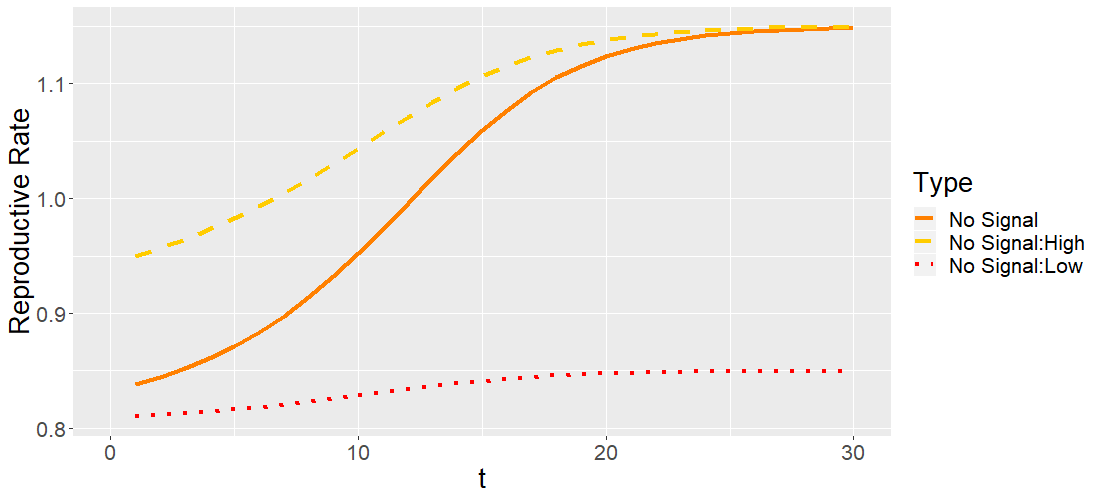
\includegraphics[width=\textwidth, height=.28\textheight]{Images/Rate_No_Signal.png}
    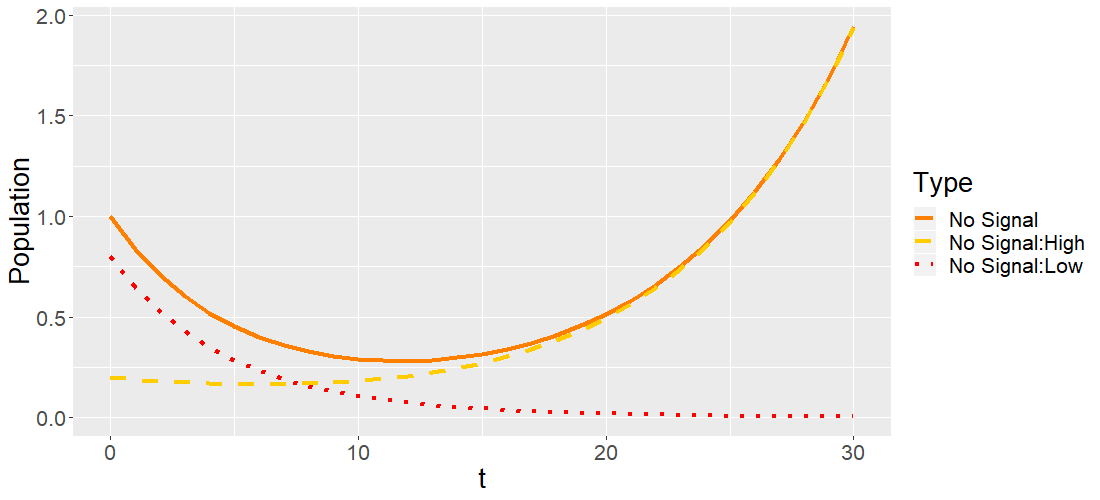
\includegraphics[width=\textwidth, height=.28\textheight]{Images/Pop_No_Signal.png}
    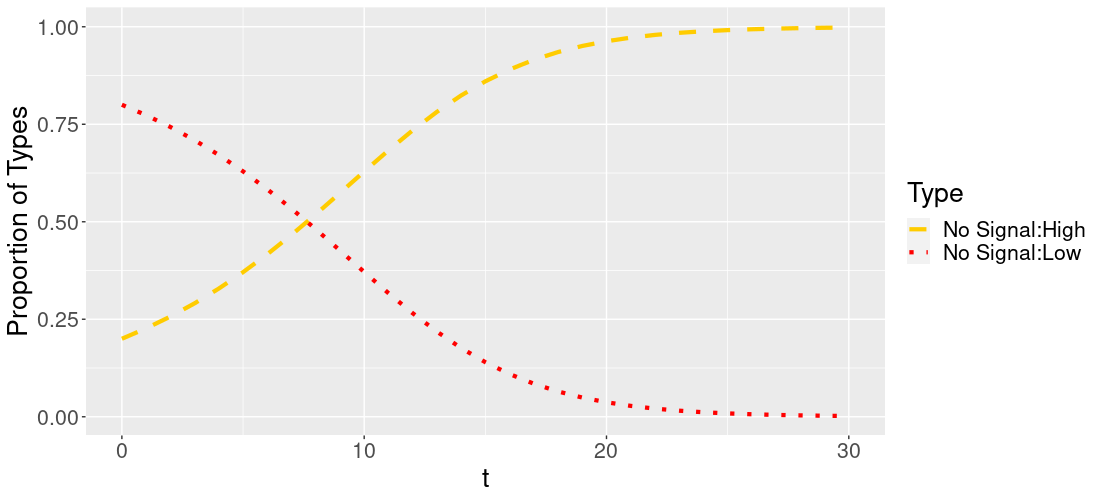
\includegraphics[width=\textwidth, height=.28\textheight]{Images/Prop_No_Signal.png}
    \begin{minipage}[c]{.2\textwidth}
    \textbf{Parameters:}
    \end{minipage}\hfill
    \begin{minipage}[c]{.2\textwidth}
    $N_0^H = .2$
    
    $N_0^L = .8$
    \end{minipage}\hfill
  \begin{minipage}[c]{.6\textwidth}
  \begin{tabular}{cc|c|c|}
      & \multicolumn{1}{c}{} & \multicolumn{1}{c}{H}  & \multicolumn{1}{c}{L} \\\cline{3-4}
      \multirow{2}*{}  & H & $1.15$ & $0.90$ \\\cline{3-4}
      & L & $0.85$ & $0.80$ \\\cline{3-4}
    \end{tabular}
    \end{minipage}
    \end{figure}

\subsection{A Population with Signaling}

 In this section we consider a population that has signaling technology. We should emphasize that here we examine behavioral signaling that individuals can choose whether to opt into. Hence, the individuals make their decisions on signaling within each generation, while the genetically determined types evolve across generations. Let $K$ be the cost of signaling. %Consistent with the handicap principle \cite{Zahavi1975} 
 We assume that the cost of signaling, $K$, is sufficiently high such that only high types can afford it.  Formally, we require: \begin{equation} \label{IC1}
     V(L,L)>V(L,H)-K.
 \end{equation}
 
Inequality (\ref{IC1}) states that the payoff for a low type by being matched with another low type is larger than the benefit of adopting the signal, a higher payoff by being matched with a high type, minus the cost of signaling. We also only want to consider signals that are potentially incentive compatible for high types. That is, a high type receives a higher payoff by being matched with another high type, even after paying the cost of signaling, than it does by being matched with a low type: \begin{equation}\label{IC2}
     V(H,H)-K>V(H,L).
 \end{equation}
 
 Combining the Inequalities \ref{IC1} and \ref{IC2}, we know that for a viable signal of cost $K$ to exist it must be the case that: \begin{equation}
     V(H,H)+V(L,L)>V(L,H)+V(H,L).
 \end{equation}
 This is known as the single crossing property \citep{Zahavi1975, Spence1973}.
 We enforce these conditions on the reproductive rates $V(.,.)$ and the cost of signaling $K$.
 
 Since we consider behavioral signaling, we assume that the individuals reach an equilibrium on their decisions on adopting the signal within each generation before reproduction. In an equilibrium, each individual has no incentive to deviate from its current choice of whether to signal. As shown in \cite{Spence1973}, given the incentive compatibility conditions (\ref{IC1}) and (\ref{IC2}), there exists a separating equilibrium in which only high types signal. Moreover, all high types are matched with one another, and low types are matched with one another, resulting in perfectly assortative matching in types. The high types earn a payoff of $V(H, H)-K$ and the low types earn a payoff of $V(L, L)$ in equilibrium. Note that the separating equilibrium is independent of the distribution of types in the population. Even when the group of low types is vanishingly small, the high types would still pay the cost of signaling to segregate themselves from the low types.

 We define the population with signaling at time $t$ as $S_t \in \mathbb{R}$ where $S_t = S^H_t + S^L_t$. Here, $S^H_t \in \mathbb{R}$ and $S^L_t \in \mathbb{R}$ are the amount of high types and low types, respectively, in the signaling population at time $t$. Because of signaling, the individuals are only matched with their own types. Hence, $S^H_t$ and $S^L_t$ experience a constant reproductive rate over time. Their evolutionary dynamics are as follows: 
\begin{eqnarray}
   && S^H_{t+1}=[V(H,H)-K]*S^H_t, \label{signaldynamic1}\\
&&     S^L_{t+1}=V(L,L)*S^L_t. \label{signaldynamic2}
\end{eqnarray}



\begin{figure}[p]
  \caption{Population Dynamics Where High Types Signal}
   \label{fig:Signal}
    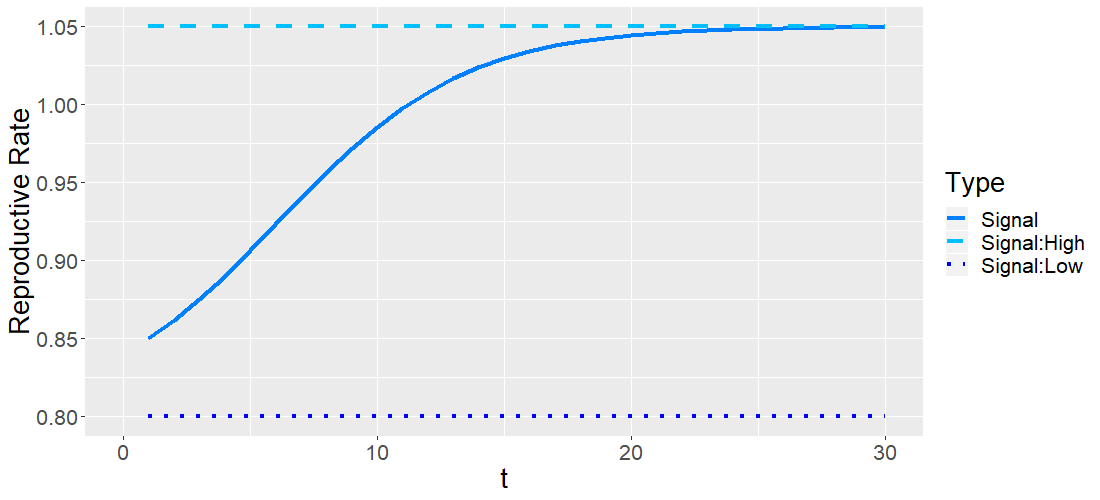
\includegraphics[width=\textwidth, height=.28\textheight]{Images/Rate_Signal.png}
    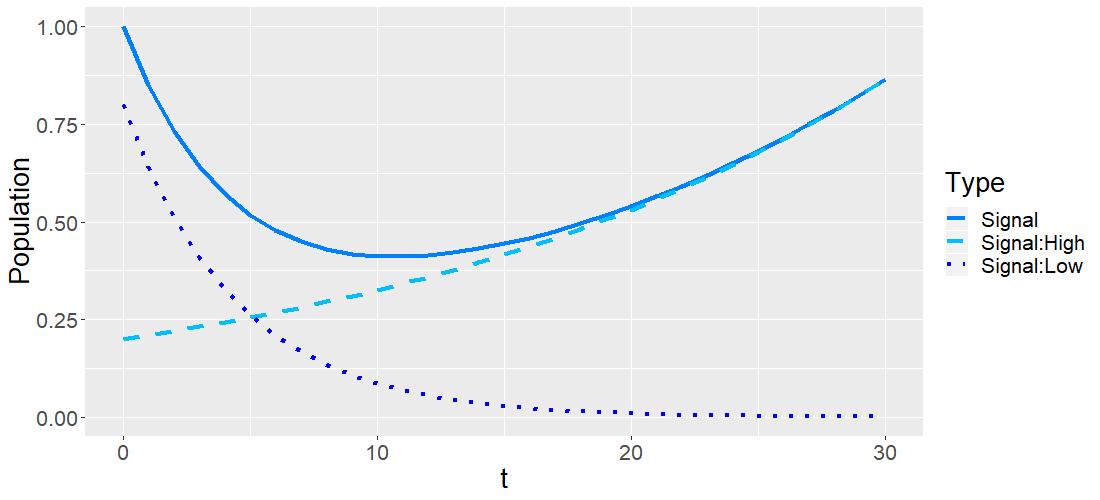
\includegraphics[width=\textwidth, height=.28\textheight]{Images/Pop_Signal.png}
    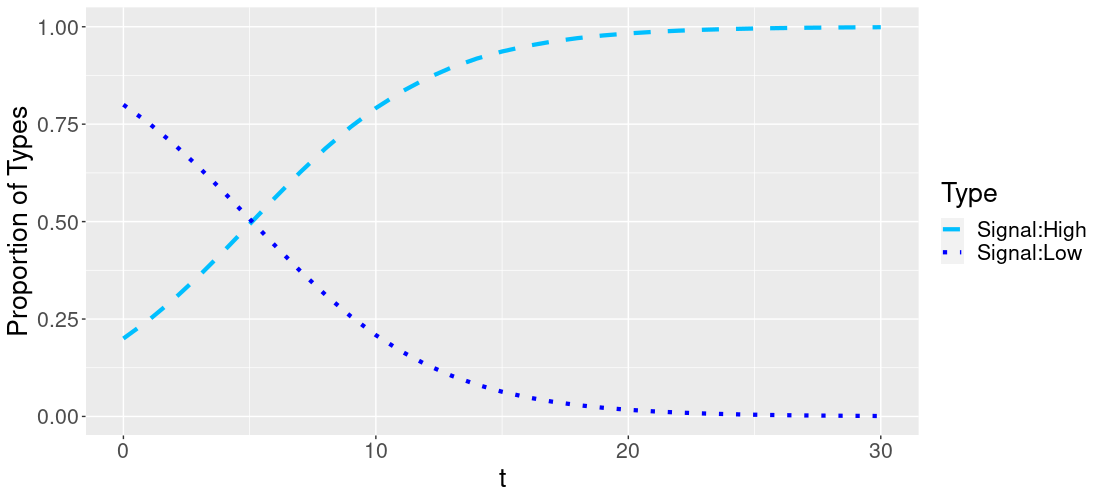
\includegraphics[width=\textwidth, height=.28\textheight]{Images/Prop_Signal.png}
 \begin{minipage}[c]{.2\textwidth}
    \textbf{Parameters:}
    \end{minipage}\hfill
    \begin{minipage}[c]{.2\textwidth}
    
    $S_0^H = .2$
    
    $S_0^L = .8$
    
    $K = .1$
    \end{minipage}\hfill
  \begin{minipage}[c]{.6\textwidth}
  \begin{tabular}{cc|c|c|}
      & \multicolumn{1}{c}{} & \multicolumn{1}{c}{H}  & \multicolumn{1}{c}{L} \\\cline{3-4}
      \multirow{2}*{}  & H & $1.15$ & $0.90$ \\\cline{3-4}
      & L & $0.85$ & $0.80$ \\\cline{3-4}
    \end{tabular}
    \end{minipage}
    \end{figure}

We simulate the dynamics described by Equations (\ref{signaldynamic1}) and \ref{signaldynamic2} in Figure \ref{fig:Signal}. We have three similar graphs as in Figure (\ref{fig:No_Signal}) and use the same parameters. Note that in the top graph, the reproductive rate of the high types and low types are not influenced by the relative size of each sub-population since they always match with their own types. This can be seen in Equations (\ref{signaldynamic1}) and (\ref{signaldynamic2}),  where the coefficients on $S^H_t$ and $S^L_t$, do not depend on the population composition. As a result, the reproductive rate of the population increases only because high types evolve to make up a greater proportion of the population. It can not be seen in the graphs here, but it should be clear that as $K$, the cost of signaling, decreases the speed of evolution increases. 


%\subsection{A Population with Signaling in a Purely Genetic Model}

%Here we differentiate from the previous section by examining signals that are non-elective such as the peacock's tail and other physical characteristics that serve as signals where the signal is indistinguishable between low and high types. As a result, much like the population without signaling, individuals are randomly matched with other individuals in their population. We define the genetic signaling population at time $t$ as $SG_t$ where $SG_t = SG^H_t + SG^L_t$. Here, $SG^H_t$ and $SG^L_t$ are the amount of high types and low types, respectively, in the non-signaling population at time $t$. Like the signaling population in the previous population signalers must pay the cost $K$ of signaling. 

%Assuming a large $GS_t$, the law of large numbers implies that $GS^H_t$ and $GS^L_t$ evolve according to their expected payoffs from Table \ref{tab:payofftable}. So we have: 
%\begin{eqnarray}
%    && GS^H_{t+1}=[\frac{GS^H_t}{GS_t}*(V(H,H)-K)+\frac{GS^L_t}{GS_t}*(V(H,L)-K)]*N^H_t, \label{signalgeneticdynamic1}\\
%    && GS^L_{t+1}=[\frac{GS^H_t}{GS_t}*(V(L,H)-K)+\frac{GS^L_t}{GS_t}*(V(L,L)-K)]*N^L_t.\label{signalgeneticdynamic2}
%\end{eqnarray}

%Add graphs for GS%

\subsection{Comparing Signaling and Non-Signaling Populations}

Figure \ref{fig:Apart} shows the overlap of Figure \ref{fig:No_Signal} and Figure \ref{fig:Signal}, both of which have the same parameters. Looking at the first graph of Figure \ref{fig:Apart}, we can see that while $N^H_t/N_t$ is sufficiently small, the reproductive rate for the signaling high types is greater than the reproductive rate for the high types in the non-signaling population. This is because $V(H,H) - K > V(H,L)$. As a result, high types evolve faster within the signaling population compared to the high types in the non-signaling population. In the first graph of Figure \ref{fig:Apart}, we can see that it takes until period 10 before the high types in the non-signaling population reach the same reproductive rate of their counterparts in the signaling population. Because of this and because low types in the signaling population have a lower reproductive rate than low types in the non-signaling population, high types make up a larger proportion of the signaling population compared to the non-signaling population. Therefore, it takes a few more periods until the average reproductive rate across the non-signaling population surpasses that of the signaling population. Looking at the second graph in Figure \ref{fig:Apart}, we can see that although the reproductive rate of the non-signaling population surpasses that of the signaling population around period 13, the signaling population retains a population advantage until around period 21. This is because the signaling population builds a significant population advantage in the initial periods. However, once sufficient time has passed and both populations are essentially homogeneous with only high types left, the non-signaling population realizes a reproductive rate that is $K$ greater than that of the signaling population. The final graph in Figure \ref{fig:Apart} shows the difference in the type makeup of the two populations. Note that the greatest difference occurs shortly after the start of the evolution but then vanishes as high types eventually make up the entirety of both populations.

\begin{figure}[p]
  \caption{Comparison of Population Dynamics Between Signaling and Non-Signaling Populations}
   \label{fig:Apart}
    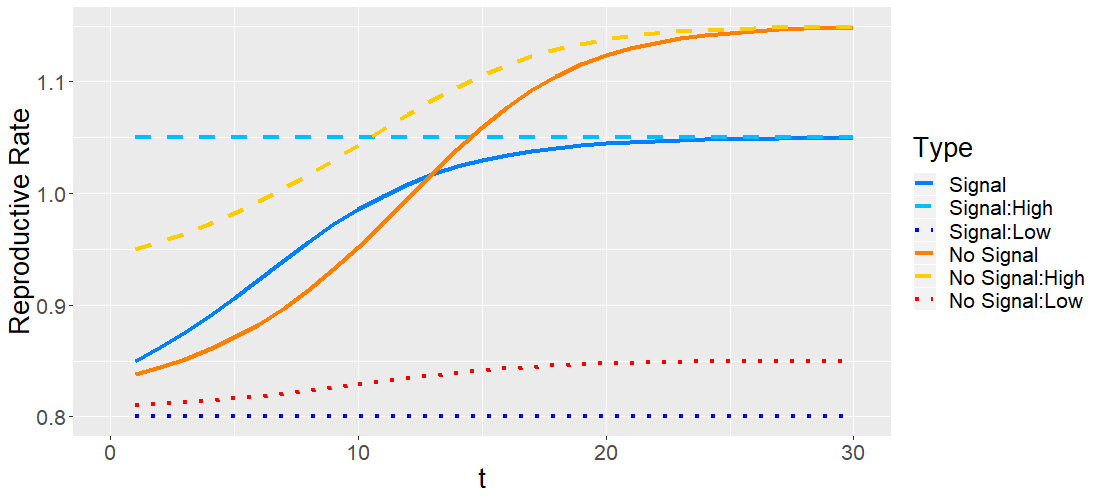
\includegraphics[width=\textwidth, height=.28\textheight]{Images/Rate_Apart.png}
    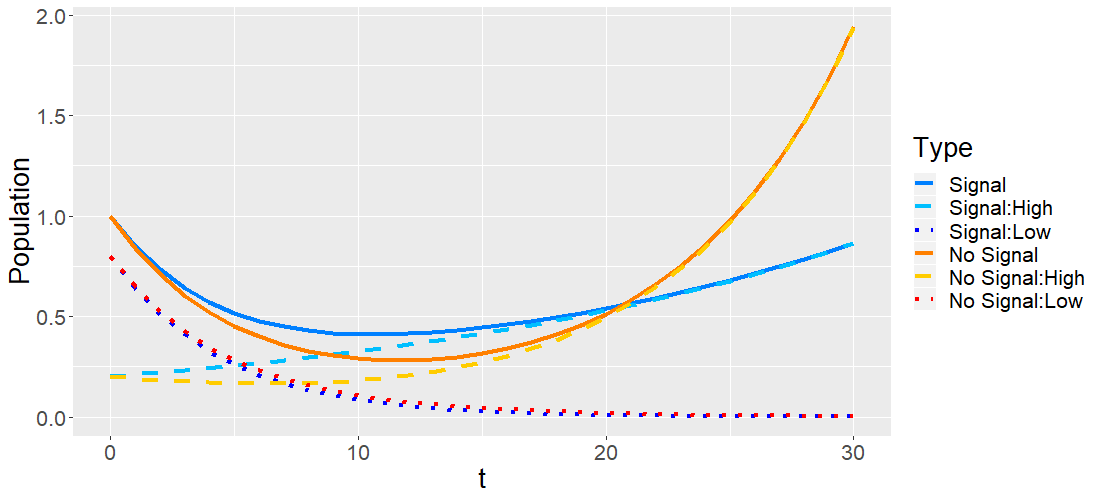
\includegraphics[width=\textwidth, height=.28\textheight]{Images/Pop_Apart.png}
    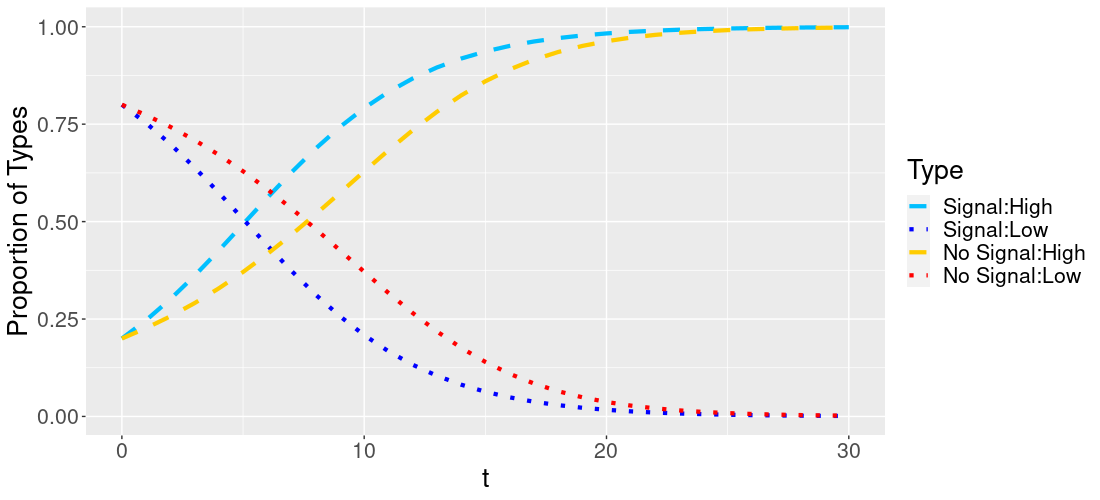
\includegraphics[width=\textwidth, height=.28\textheight]{Images/Prop_Apart.png}
 \begin{minipage}[c]{.2\textwidth}
    \textbf{Parameters:}
    \end{minipage}\hfill
    \begin{minipage}[c]{.2\textwidth}
    
    $N_0^H = S_0^H = .2$
    
    $N_0^L = S_0^L = .8$
    
    $K = .1$
    \end{minipage}\hfill
  \begin{minipage}[c]{.6\textwidth}
  \begin{tabular}{cc|c|c|}
      & \multicolumn{1}{c}{} & \multicolumn{1}{c}{H}  & \multicolumn{1}{c}{L} \\\cline{3-4}
      \multirow{2}*{}  & H & $1.15$ & $0.90$ \\\cline{3-4}
      & L & $0.85$ & $0.80$ \\\cline{3-4}
    \end{tabular}
    \end{minipage}
    \end{figure}


\subsection{Conflicts between the Two Populations}

Assume that in period $T$ the non-signaling population and the signaling population engage in conflicts. In periods $t \in [0,T)$ the populations evolve according to the dynamics in the above sections, but starting at period $T$ they start to eliminate the other population according to the Lanchester's square law \citep{Lanchester1916}. The Lanchester's square law has been applied to a variety of human and non-human conflicts. See for example \cite{Wilsonetal2002}, \cite{JohnsonMackay2015EHB} and \cite{clifton2020brief}.\footnote{Another common way of modeling intergroup conflict is to treat it as a game played between two groups. Individuals within a group can contribute to the group's effort, which is costly to themselves, but beneficial to the group collectively in the conflict. Hence, an individual may have an incentive to free ride on fellow group members. See \cite{Bornstein2003} for a review. Since our focus is on signaling behavior, we refrain from complicating the model by adding an extra layer of effort choice.} In each period, before reproduction, each member of a population kills $\beta$ members of the other population. Individuals that are killed are drawn uniformly from the population. Parameter $\beta$ reflects how efficient the weapons used in the conflicts are. Hence, the dynamics for $N^H, N^L, S^H,$ and $S^L$ are now given as:
\begin{eqnarray}
    && N^H_{t+1}=[\frac{N^H_t}{N_t}*V(H,H)+\frac{N^L_t}{N_t}*V(H,L)]*max\{[N^H_t-\beta \frac{N^H_t}{N_t} I_{t \geq T}S_t],0\},
\\
&& N^L_{t+1}=[\frac{N^H_t}{N_t}*V(L,H)+\frac{N^L_t}{N_t}*V(L,L)]*max\{[N^L_t-\beta \frac{N^L_t}{N_t} I_{t \geq T}S_t],0\},
\\
    && S^H_{t+1}=[V(H,H)-K]*max\{[S^H_t-\beta \frac{S^H_t}{S_t} I_{t \geq T}N_t],0\},
\\
  && S^L_{t+1}=V(L,L)*max\{[S^L_t-\beta \frac{S^L_t}{S_t} I_{t \geq T}N_t],0\}.
\end{eqnarray}

In the equations above, $I_{t \geq T}$ is an indicator that the groups are engaging in inter-group conflicts and the max argument simply ensures that the populations would not reach a negative number. Note that we specify that conflicts take place before reproduction in each period in this model. It is clear that when applying this model, the time between each discrete period would simply be the amount of time it takes for a generation to reproduce. While conflicts may run at a different time scale, we can force conflicts into the reproduction time scale by adjusting the value of $\beta$. 

\begin{figure}[p]
  \caption{Conflicts Between Signaling and Non-Signaling Populations After a Period of Peace}
   \label{fig:Fight}
    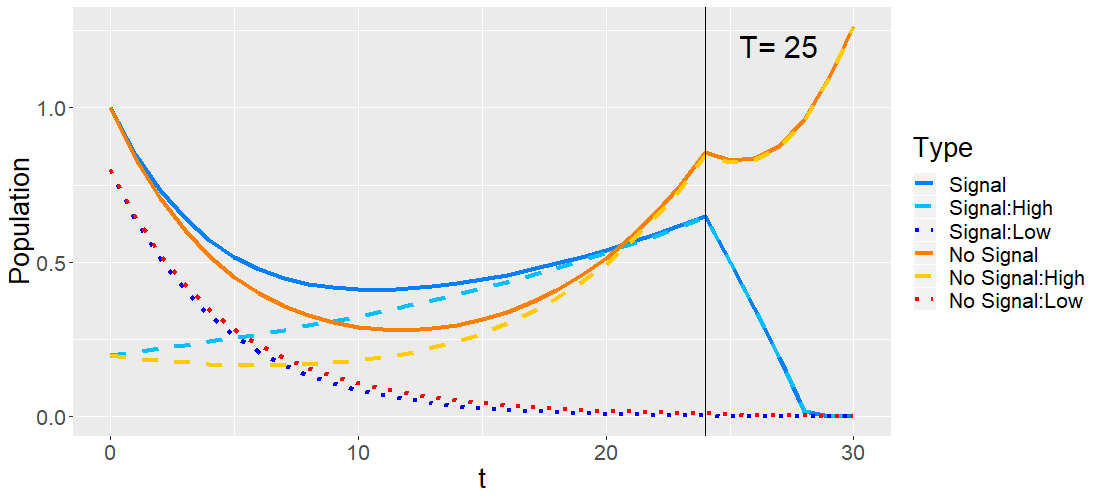
\includegraphics[width=\textwidth, height=.28\textheight]{Images/Fight_NS_Win.png}
    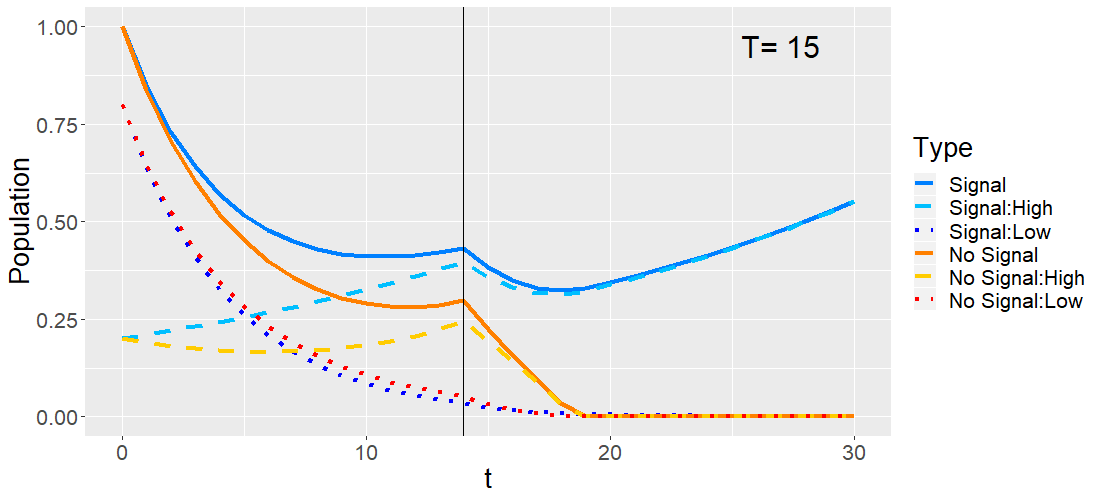
\includegraphics[width=\textwidth, height=.28\textheight]{Images/Fight_S_Win.png}
    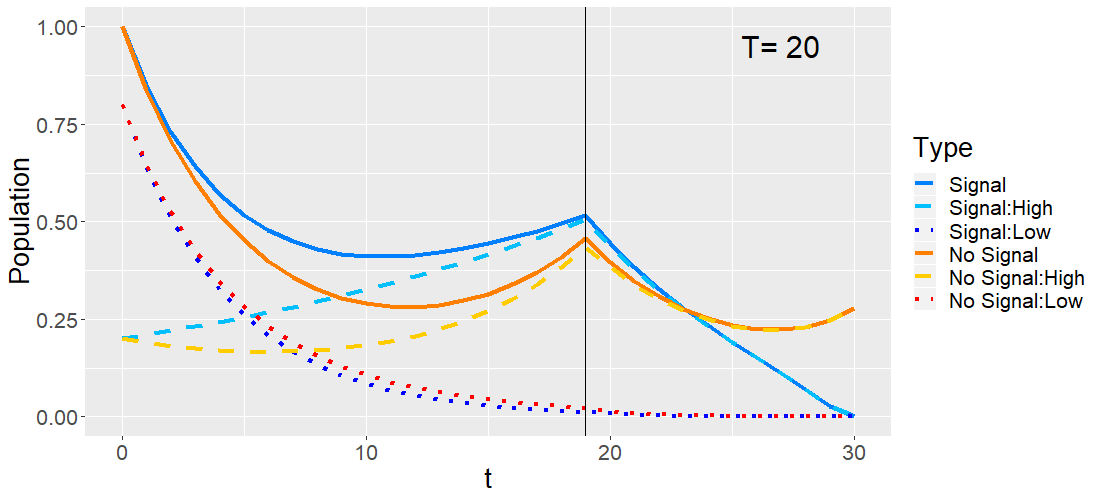
\includegraphics[width=\textwidth, height=.28\textheight]{Images/Fight_Special.png}
 \begin{minipage}[c]{.2\textwidth}
    \textbf{Parameters:}
    \end{minipage}\hfill
    \begin{minipage}[c]{.2\textwidth}
    
    $N_0^H = S_0^H = .2$
    
    $N_0^L = S_0^L = .8$
    
    $K = .1$
    
    $\beta = .2$
    \end{minipage}\hfill
  \begin{minipage}[c]{.3\textwidth}
  \begin{tabular}{cc|c|c|}
      & \multicolumn{1}{c}{} & \multicolumn{1}{c}{H}  & \multicolumn{1}{c}{L} \\\cline{3-4}
      \multirow{2}*{}  & H & $1.15$ & $0.90$ \\\cline{3-4}
      & L & $0.85$ & $0.80$ \\\cline{3-4}
    \end{tabular}
    \end{minipage}\hfill
    \begin{minipage}[c]{.3\textwidth}
    The vertical lines indicate the last period before conflicts begin $(T-1)$.
    \end{minipage}
    \end{figure}

Figure \ref{fig:Fight} provides three examples of outcomes when conflicts occur in our model. In the top graph, the non-signaling population enters the periods of conflicts with a population advantage. Because they do not need to pay the cost of signaling, the fact that they have a population advantage indicates that they also have a superior reproductive rate. As a result, the non-signaling population always wins. In the second graph, the signaling population enters the conflicts with a population advantage. At this point the signaling population doesn't necessarily have a higher reproductive rate, however, if weapon used in conflicts is sufficiently efficient ($\beta$ is sufficiently large), the signaling population will be able to eliminate the non-signaling population before the non-signaling population can catch up with their superior long run reproductive rate. The third graph is a special case. Although the signaling population enters the conflicts with a slightly larger population, because $\beta$ is sufficiently small, the non-signaling population is able to overcome the signaling population during the conflicts.


\section{Comparative Statics}

\begin{figure}[p]
  \caption{Conflicts Between Signaling and Non-Signaling Populations After a Period of Peace: Comparative Statics}
   \label{fig:Regions}
    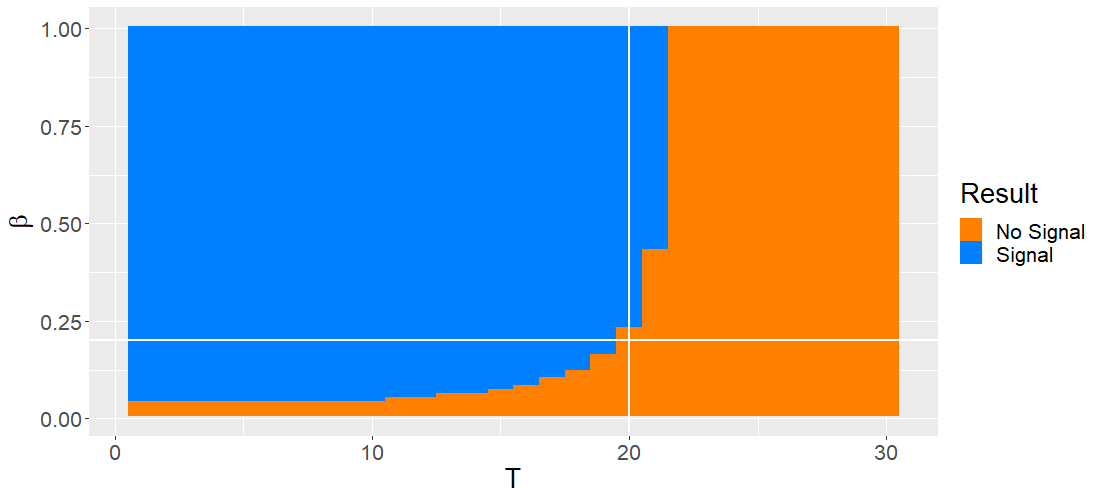
\includegraphics[width=\textwidth, height=.28\textheight]{Images/Region_BT.png}
    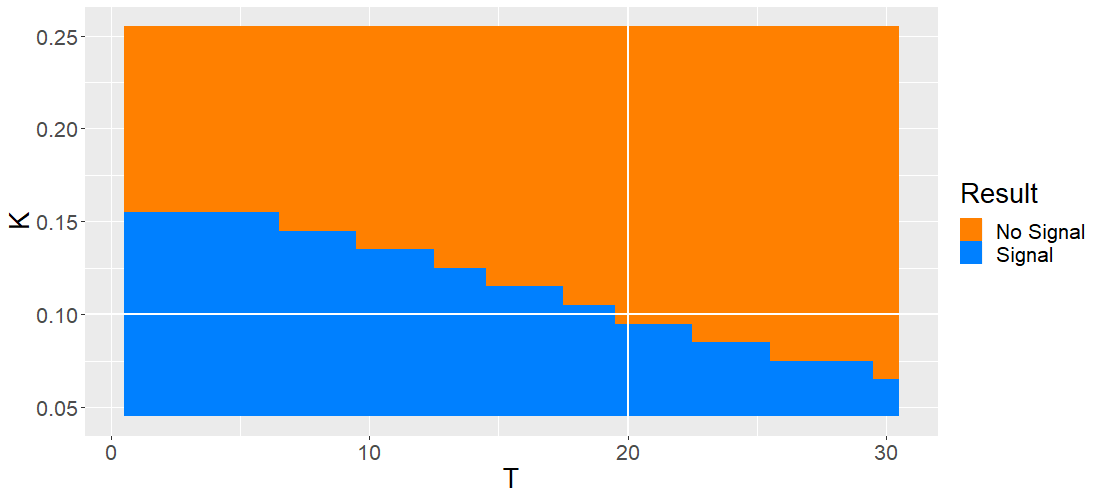
\includegraphics[width=\textwidth, height=.28\textheight]{Images/Region_KT.png}
    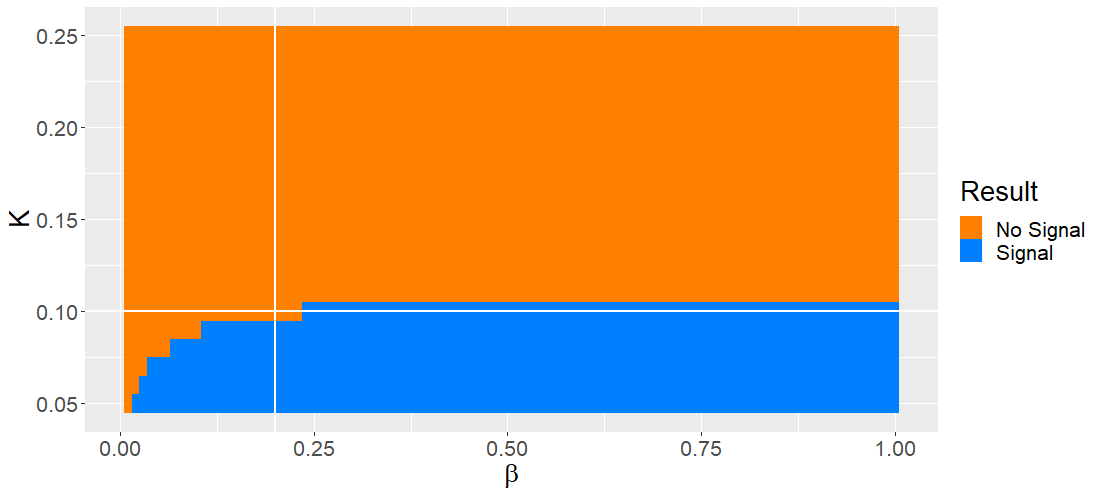
\includegraphics[width=\textwidth, height=.28\textheight]{Images/Region_KB.png}
 \begin{minipage}[c]{.2\textwidth}
    \textbf{Parameters:}
    \end{minipage}\hfill
    \begin{minipage}[c]{.2\textwidth}
    
    $N_0^H = S_0^H = .2$
    
    $N_0^L = S_0^L = .8$
    
    $K = .1$
    
    $\beta = .2$
    
    $T = 20$
    \end{minipage}\hfill
  \begin{minipage}[c]{.3\textwidth}
  \begin{tabular}{cc|c|c|}
      & \multicolumn{1}{c}{} & \multicolumn{1}{c}{H}  & \multicolumn{1}{c}{L} \\\cline{3-4}
      \multirow{2}*{}  & H & $1.15$ & $0.90$ \\\cline{3-4}
      & L & $0.85$ & $0.80$ \\\cline{3-4}
    \end{tabular}
    \end{minipage}\hfill
    \begin{minipage}[c]{.3\textwidth}
    The white intercept lines indicate the current parameters values. 
    \end{minipage}
    \end{figure}
    
We have shown that costly signaling in a population may be competitively advantageous in inter-group conflicts in our model. The viability of signaling depends largely on three different factors: the period that conflicts start ($T$), the cost of signaling ($K$), and the efficiency of weapon used in conflicts ($\beta$). Here, we argue that the signaling population benefits from a shorter period of isolation before conflicts, a smaller cost of signaling, and more efficient weapon used in conflicts. To clearly see the effects of these three factors, we run the model thousands of different times, varying the key parameters: $T,K$ and, $\beta$ and indicate the outcomes of the conflicts. The results are reported in Figure \ref{fig:Regions}, in which each pixel plotted corresponds to the outcome of the evolution given a set of parameters. In areas colored orange, the non-signaling population wins the conflicts and in the blue area the signaling population wins. The white intercept lines indicate where the model is evaluated in the last graph of Figure \ref{fig:Fight}.

The first graph in Figure \ref{fig:Regions} shows the result of the conflicts between the signaling population and the non-signaling population as we vary the period that conflicts start and the efficiency of weapon used in conflicts. As we can see, beyond a certain period the non-signaling population will always win no matter what the value of $\beta$ is. This is because the  non-signaling population is both greater and growing faster beyond that period. One can verify this by looking at Figure \ref{fig:Apart}. It is also necessary for $\beta$ to be sufficiently large for the signaling population to possibly win the conflicts. As we can see, when $\beta$ is sufficiently small, the non-signaling population always wins. Looking at the second graph of Figure \ref{fig:Regions}, we can see that a smaller signaling cost benefits the signaling population. The third graph of Figure \ref{fig:Regions} shows the interaction between the cost of signaling and the efficiency of weapon used in conflicts at $T=20$. The non-signaling population always wins when $K>.1$ because the non-signaling would have a larger population than the signaling population at $T=20$. Before that point, more efficient weapon used in conflicts can compensate for a higher cost of signaling for the signaling population.  

Please note that thus far we have used $N_0^H = .2$ and $N_0^L = .8$ and $S_0^H = .2$ and $S_0^L = .8$. Recall that high types are the individuals that are better suited to their current environment and thus have a higher fitness than low types. With this in mind, it is useful to think about the initial values of $N_0^H, N_0^L, S_0^H,$ and $S_0^L$ as being related to the speed at which the environment is changing around the people. 
The faster the environment changes, the less time passes before a new genetic mutation is considered the high type which would essentially restart our model with a small proportion of high types. So, a faster changing environment would translate to a smaller initial proportion of high types. 
With that in mind, Figure \ref{fig:RatioRegions} shows the results of the conflicts when we vary the initial proportion of high types in each population, $N_0^H$ and $S_0^H$, while keeping them consistent across populations, $N_0^H = S_0^H$, and maintaining $N_0 = S_0 = 1$ so that $N_0^H$ and $S_0^H$ is simply the initial proportion of high types in each population. The results are clear: The smaller the initial proportion of high types, the more likely it is that the signaling population will win the conflicts. 
This is because the assortative advantage is largest when the proportion of high types is smallest which further exaggerates the speed at which the makeup of the population changes from low type to high type. Hence, giving the populations more room to evolve naturally favors the signaling population. Abstracting from the model, this implies that signaling is more advantageous the quicker one's environment changes. In a rapidly changing environment, the amount of high types at any given time is expected to be lower than in a slow changing environment since we define high types as those best adapted to the current environment. As can be seen in the graphs, the smaller the initial proportion of high types, the wider the range of $T, K$ and $\beta$ values that result in conflicts that favors the signaling population.


\begin{figure}[p]
  \caption{Conflicts Between Signaling and Non-Signaling Populations After a Period of Peace: Initial Conditions Comparative Statics}
   \label{fig:RatioRegions}
    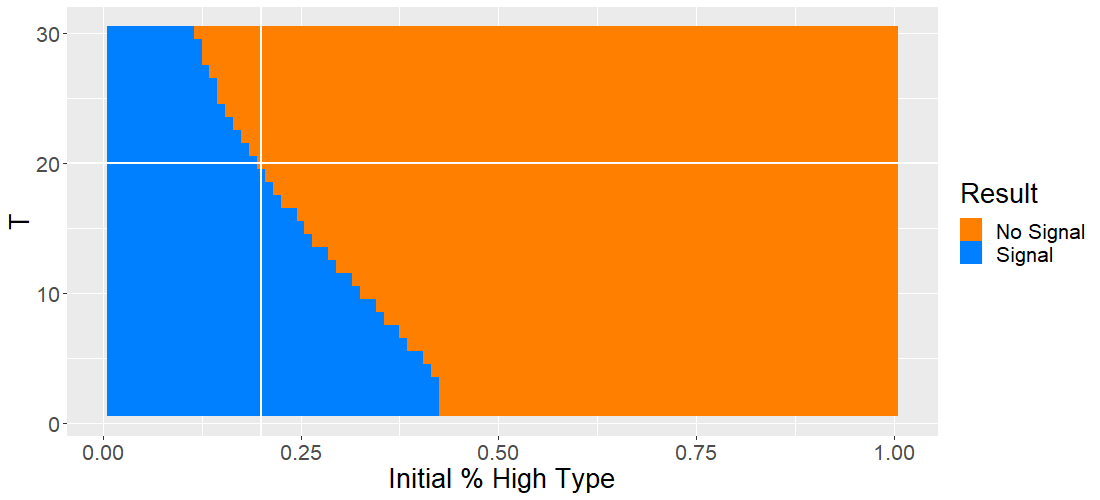
\includegraphics[width=\textwidth, height=.28\textheight]{Images/Region_RT.png}
    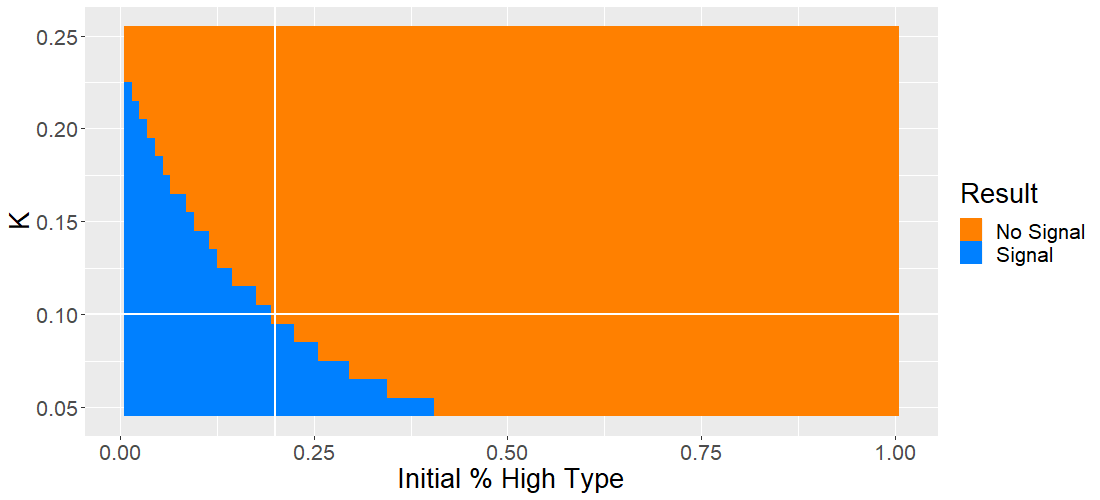
\includegraphics[width=\textwidth, height=.28\textheight]{Images/Region_RK.png}
    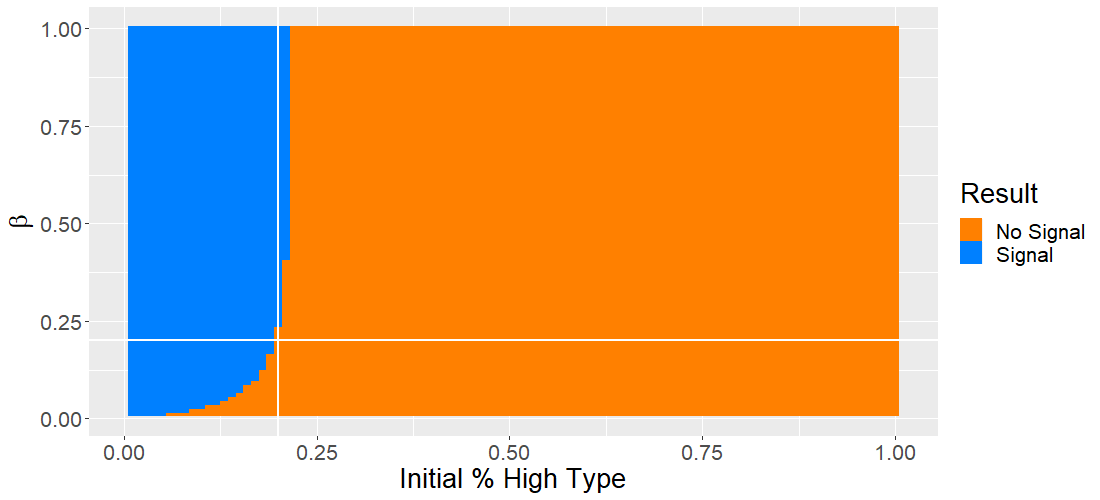
\includegraphics[width=\textwidth, height=.28\textheight]{Images/Region_RB.png}
 \begin{minipage}[c]{.2\textwidth}
    \textbf{Parameters:}
    \end{minipage}\hfill
    \begin{minipage}[c]{.2\textwidth}
    
    $N_0^H = S_0^H = .2$
    
    $N_0^L = S_0^L = .8$
    
    $K = .1$
    
    $\beta = .2$
    
    $T = 20$
    \end{minipage}\hfill
  \begin{minipage}[c]{.3\textwidth}
  \begin{tabular}{cc|c|c|}
      & \multicolumn{1}{c}{} & \multicolumn{1}{c}{H}  & \multicolumn{1}{c}{L} \\\cline{3-4}
      \multirow{2}*{}  & H & $1.15$ & $0.90$ \\\cline{3-4}
      & L & $0.85$ & $0.80$ \\\cline{3-4}
    \end{tabular}
    \end{minipage}\hfill
    \begin{minipage}[c]{.3\textwidth}
    The white intercept lines indicate the current parameters values. 
    \end{minipage}
    \end{figure}



When competition erupts or is ongoing, the eventual winner can be determined by examining the relative population levels as well as the type distribution within those populations.

 \begin{figure}[h]
   \caption{Relative Population Needed for Signaling Population to Win in Conflict}
   \label{fig:FightProps}
    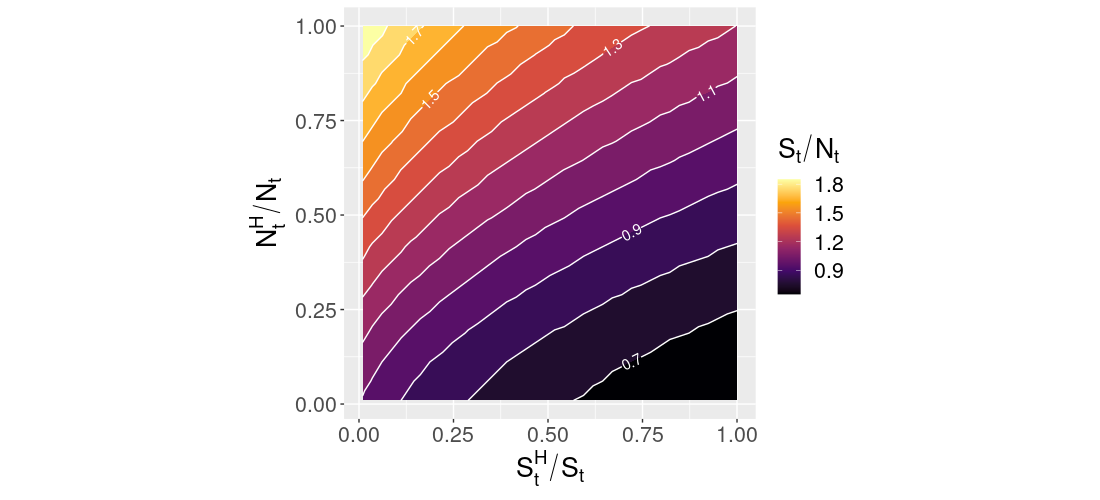
\includegraphics[width=\textwidth, height=.33\textheight]{Images/FightBoundary.png}
    \begin{minipage}[c]{.2\textwidth}
    \textbf{Parameters:}
    \end{minipage}\hfill
    \begin{minipage}[c]{.2\textwidth}
    
    $K = .1$
    
    $\beta = .2$
    
    \end{minipage}\hfill
  \begin{minipage}[c]{.3\textwidth}
  \begin{tabular}{cc|c|c|}
      & \multicolumn{1}{c}{} & \multicolumn{1}{c}{H}  & \multicolumn{1}{c}{L} \\\cline{3-4}
      \multirow{2}*{}  & H & $1.15$ & $0.90$ \\\cline{3-4}
      & L & $0.85$ & $0.80$ \\\cline{3-4}
    \end{tabular}
    \end{minipage}\hfill
    \begin{minipage}[c]{.3\textwidth}
    \end{minipage}
\end{figure}

Figure \ref{fig:FightProps} depicts the minimum relative population level ($S_t/N_t$) needed for the signaling population to defeat the non-signaling population once conflict is ongoing given the type makeup of each population. Since a greater proportion of high types increases the reproductive rate in each population, as the proportion of high types in the signaling population, $S_t^H/S_t$ increases, a smaller relative population level, $S_t/N_t$ is needed for the signaling population to win. The inverse is true for increases in the proportion of high types in the non-signaling population, $N_t^H/N_t$.



%Add section talking about pure genetic, section talking about both low and high type signalers in same population%

%Add small section in comment for "what if" to section 4%

%Low and high type signalers doesn't make sense. The signal must be an indicator of quality otherwise it is just a costly trait/behavior with no benefit because the receiver would be unable to discern quality. The signal must be tied to the quality otherwise the signal holds no value and could not evolve.%
  


\section{Discussions}
%Add subsection: alternative modeling - "what if" 1 population%

\subsection{Alternative Modeling Choices}
%In this section, we explore the possibility of considering genetic signaling, and getting rid of competition. 
\subsubsection{Low Types also Signal}
In our model we assume that in the signaling population only high types transmit a signal and as a result, the signal enforces perfect assortative matching within the signaling population. One may question what if the signal is ubiquitous across the signaling population such that low types as well as high types transmit the signal. In this case, the signal would not be a signal at all but just a costly trait since no one would be able to distinguish one type from another. As a result, the one difference between the evolutionary dynamics of the signaling and non-signaling population would be that the signaling population experiences a level decrease in their reproductive rate with no functional assortativity advantage. The only scenarios where the signaling population is able the beat the non-signaling population in conflicts in this setup are with extreme parameter values where the signaling cost and the expression $V(H,H)-V(H,L)$ are so large that the low types in the signaling population are effectively eliminated by the signaling cost immediately, thus effectively giving the high types assortative matching which, if the initial proportion of high types in each population is low enough, may allow for a very narrow window under which the signaling population will realize a population advantage. 

\subsubsection{One Population of Signalers and Non-Signalers}
Another question one may have is what if there are both signalers and non-signalers in the same population. In this case, so long as the signaling high types are able to gain an assortative advantage over the non-signaling high types in the population, then that may be enough to offset the signal cost and realize a higher reproductive rate for them in the short run even in the absence of inter-group conflicts. We demonstrate that this is not the case in a one-population model with four types (signaling high type, non-signaling high type, signaling low type, non-signaling low type) as shown in Figure \ref{fig:One_Pop}. The rationale is as follows. In our settings, high types evolve to make up an increasing proportion of the population with certainty as time increases until there are only high types remaining. As a result, at some point the relative difference in assortativity between the signaling high types and the non-signaling high types will not be big enough to offset the cost of signaling. Therefore, absent conflicts between the signalers and non-signalers, non-signaling high types will dominate the entire population with certainty in the long run.

The above discussions on alternative modelling choices suggest that signalling being behavioral (only high types choose to adopt it) and conflicts between the signaling population and the non-signaling population  are prerequisites for signaling to survive.

\begin{figure}[hp]
   \caption{One Population Where Some High Types Signal and Some Don't}
   \label{fig:One_Pop}
    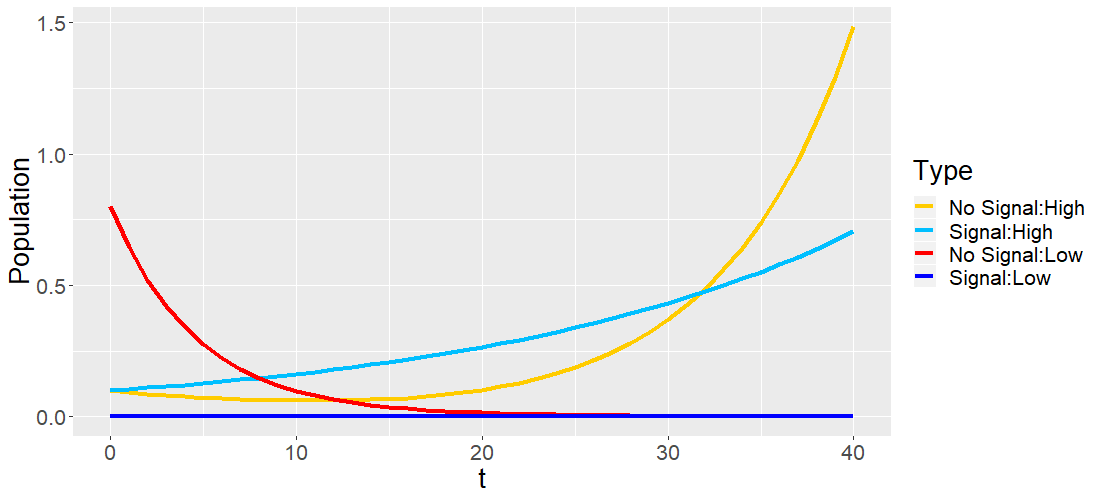
\includegraphics[width=\textwidth, height=.28\textheight]{Images/One_Pop.png}
 \begin{minipage}[c]{.2\textwidth}
    \textbf{Parameters:}
    \end{minipage}\hfill
    \begin{minipage}[c]{.2\textwidth}
    
    $N_0^H = S_0^H = .1$
    
    $N_0^L = .8$
    
    $S_0^L = 0$
    
    $K = .1$

    \end{minipage}\hfill
  \begin{minipage}[c]{.3\textwidth}
  \begin{tabular}{cc|c|c|}
      & \multicolumn{1}{c}{} & \multicolumn{1}{c}{H}  & \multicolumn{1}{c}{L} \\\cline{3-4}
      \multirow{2}*{}  & H & $1.15$ & $0.90$ \\\cline{3-4}
      & L & $0.85$ & $0.80$ \\\cline{3-4}
    \end{tabular}
    \end{minipage}\hfill
    \begin{minipage}[c]{.3\textwidth}

    \end{minipage}
    \end{figure}
\newpage
\subsubsection{Imperfect Signaling}

In the dynamics explored in this paper, we assumed agents always made the payoff maximizing choice which led to perfect assortativity in the signaling population. This perfect assortativity allowed the signaling population to gain a temporary reproductive edge over the non-signaling population. Here we will relax the assumption of perfect associativity and instead examine how our model behaves where there is a probability $p$ that agents make a mistake and signal when they shouldn't (low types) or not signal when they should (high types). $1-p$ measures the accuracy of signaling.\footnote{Essentially, we endogenize the degree of assortative matching through imperfect signaling. See \cite{NaxRigos2016}, \cite{Newton2017IJGT}, \citet{wu2016,wu2018,wu2023wp} for the study of endogenous assortativity through different mechanisms.} Intuitively, $p$ should be some value in the range $[0,1/2)$ as $p=0$ implies mistake free signaling and $p=1/2$ implies signaling is entirely uninformative. As such, the payoffs realized by each type is no longer fixed and now depends on the proportion of high types to low types within the population as a whole. Note that the dynamics in the non-signaling population remain unchanged by this assumption. 

If high types imperfectly signal and low types imperfectly choose not to signal that means that $S^H_t*(1-p) + S^L_t*p$ describes the total number of signalers and $S^H_t*p + S^L_t*(1-p)$ describes the total number of non-signalers at time $t$.

Assuming that high types choose to signal and low types choose to not signal, and match according to their signal. When a high type does signal, the payoff they get is given by the following expression:
\setlength{\belowdisplayskip}{4pt} \setlength{\belowdisplayshortskip}{4pt}
\setlength{\abovedisplayskip}{4pt} \setlength{\abovedisplayshortskip}{4pt}
\begin{eqnarray}
&& A \equiv V(H,H) * \frac{S^H*(1-p)}{S^H*(1-p)+S^L*p} + V(H,L) * \frac{S^L*p}{S^H*(1-p)+S^L*p} - K. \label{imperfectsignaldynamic1}
\end{eqnarray}

When a high type does not signal, the payoff they get is given by the following expression:
\begin{eqnarray}
&& B \equiv V(H,H) * \frac{S^H*p}{S^H*p+S^L*(1-p)} + V(H,L) * \frac{S^L*(1-p)}{S^H*p+S^L*(1-p)}. \label{imperfectsignaldynamic2}
\end{eqnarray}

As such, in order for choosing to signal to be incentive compatible for high types the following relation must hold:
$(1-p)*A + p*B > p*A + (1-p)*B.$ Given that $p \in [0,1/2)$, this can be simplified to: $A > B$.

%We can pull a $V(H,H)$ out of A and pull a $V(H,L)$ out of B which results in the following inequality:
%\begin{eqnarray}
%&& 
%\begin{split}
%V(H,H) - \frac{S^L*p}{S^H*(1-p)+S^L*p}(V(H,H)-V(H,L)) - K > \\
%V(H,L) + \frac{S^H*p}{S^H*p+S^L*(1-p)}(V(H,H)-V(H,L)).
%\end{split}
%\label{imperfectsignaldynamic5}
%\end{eqnarray}
%This can be simplified to:

The inequality $A>B$ can be rewritten as:
\begin{eqnarray}
&& (V(H,H) - V(H,L))*(1-\frac{S^L*p}{S^H*(1-p)+S^L*p}-\frac{S^H*p}{S^H*p+S^L*(1-p)}) > K. \label{imperfectsignaldynamic6}
\end{eqnarray}

This inequality sets the upper bound on viable signal cost $K$. Since $p \in [0,1/2)$, and $V(H,H)>V(H,L)$, the left hand side term is positive if $S^L, S^H \neq 0$ which means there can exist a positive signaling cost $K$ under which high types are incentivized to signal. 

Likewise, when a low type does signal, the payoff they get is given by the following expression:
\begin{eqnarray}
&& C \equiv V(L,H) * \frac{S^H*(1-p)}{S^H*(1-p)+S^L*p} + V(L,L,) * \frac{S^L*p}{S^H*(1-p)+S^L*p} - K. \label{imperfectsignaldynamic7}
\end{eqnarray}

When a low type does not signal, the payoff they get is given by the following expression:
\begin{eqnarray}
&& D \equiv V(L,H) * \frac{S^H*p}{S^H*p+S^L*(1-p)} + V(L,L,) * \frac{S^L*(1-p)}{S^H*p+S^L*(1-p)}. \label{imperfectsignaldynamic8}
\end{eqnarray}

As such, in order for choosing to not signal to be incentive compatible for low types the following relation must hold: $(1-p)*C + p*D < p*C + (1-p)*D.$ Given that $p \in [0,1/2)$, this can be simplified to: $ C < D$. 
%We can pull a $V(L,H)$ out of C and a $V(L,L)$ out of D which results in the following inequality:
%\begin{eqnarray}
%&& 
%\begin{split}
%V(L,H) - \frac{S^L*p}{S^H*(1-p)+S^L*p}(V(L,H)-V(L,L)) - K < \\
%V(L,L) + \frac{S^H*p}{S^H*p+S^L*(1-p)}(V(L,H)-V(L,L)).
%\end{split}
%\label{imperfectsignaldynamic11}
%\end{eqnarray}
%
%This can be simplified to:

The inequality $C>D$ can be rewritten as:
\begin{eqnarray}
&& (V(L,H) - V(L,L))*(1-\frac{S^L*p}{S^H*(1-p)+S^L*p}-\frac{S^H*p}{S^H*p+S^L*(1-p)}) < K. \label{imperfectsignaldynamic12}
\end{eqnarray}

This inequality sets the lower bound for incentive compatible levels of $K$. Since $p \in [0,1/2)$, the term $1-\frac{S^L*p}{S^H*(1-p)+S^L*p}-\frac{S^H*p}{S^H*p+S^L*(1-p)}\in (0,1]$. In effect, an increase in $p$ decreases the lower bound on $K$. 

Combining inequalities [\ref{imperfectsignaldynamic6}] and [\ref{imperfectsignaldynamic12}] we get the following expression:
\begin{eqnarray}
&& 
\begin{split}
(V(H,H) - V(H,L))*(1-\frac{S^L*p}{S^H*(1-p)+S^L*p}-\frac{S^H*p}{S^H*p+S^L*(1-p)}) > K > \\
(V(L,H) - V(L,L))*(1-\frac{S^L*p}{S^H*(1-p)+S^L*p}-\frac{S^H*p}{S^H*p+S^L*(1-p)}).
\end{split}
\label{imperfectsignaldynamic13}
\end{eqnarray}


 
 \begin{figure}[h]
   \caption{Range of Viable Signal Costs (K) by Signal Accuracy (1-p) and Degree of Heterogeneity}
   \label{fig:ViableK}
    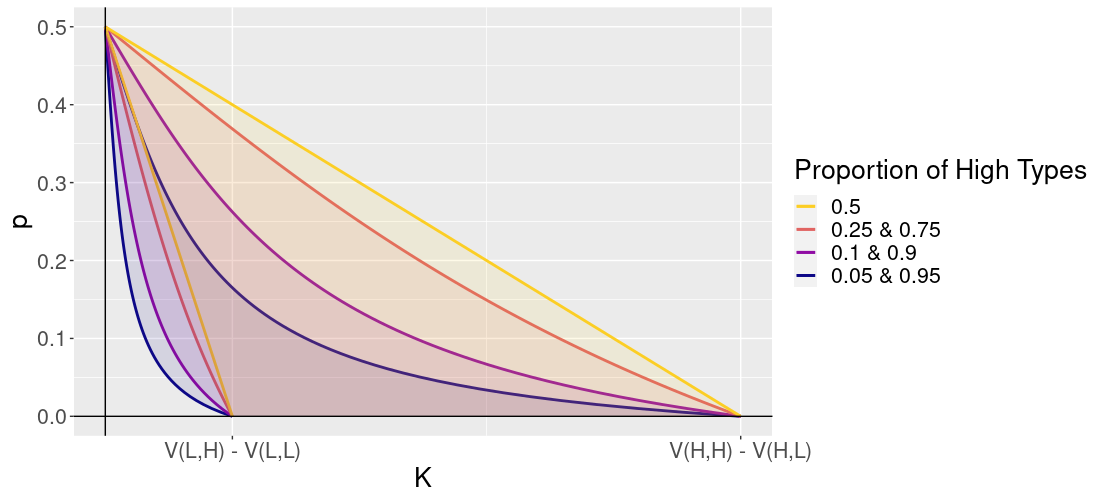
\includegraphics[width=\textwidth, height=.28\textheight]{Images/ViableK2.png}
    \end{figure}
 
 Figure \ref{fig:ViableK} shows how the accuracy of signaling ($1-p$) and the degree of heterogeneity within the entire population  (measured by $\min\{\frac{S^H}{S^H+S^L}, \frac{S^H}{S^H+S^L}\}$) affect viable levels of costly signaling ($K$) that give a separating equilibrium. Note that as the accuracy of signaling or heterogeneity decrease, the range of viable signal costs ($K$) decreases and approaches zero. This can be seen mathematically in equation [\ref{imperfectsignaldynamic13}] by taking the limit of the leftmost and rightmost terms as 1) $p$ approaches $1/2$, or as 2) $S^L$ or 3) $S^H$ approaches $0$. In all three cases, the limit of the terms is equal to $0$, thus collapsing the inequality. In each case, this is because the assortative benefit to signaling decreases as signaling accuracy or heterogeneity decreases. In the first case, when $p$ increases and approaches $1/2$, the decision to signal becomes less and less precise. As result, the assortativity within populations decreases. When signaling is imperfect ($p>0$) and heterogeneity decreases, the difference in type distribution between the signalers and non-signalers decreases. As $S^H$ or $S^L$ approaches $0$ (i.e., heterogeneity goes to $0$), the type distribution of signalers and that of non-signalers converge.
 
 The assortative benefit of signaling when signaling is imperfect is maximized when the entire population is most heterogeneous. This can be seen in Figure \ref{fig:Homogeneity}. This graph shows the types of equilibria reached under different values of $K$ and degrees of heterogeneity with a fixed $p \in (0,1/2)$. This graph shows that as a population evolves from almost all low types to almost all high types with a fixed signal cost $K$, the type of equilibrium in the population can change, in some cases several times. First, suppose $K < (V(L,H) - V(L,L))*(1-2p)$. When the degree of heterogeneity is sufficiently low, the separating equilibrium inequality fails because the assortative benefit is not large enough for the high types to signal (as discussed in the previous paragraph). When the degree of heterogeneity is sufficiently high, the separating equilibrium inequality fails again  because it is no longer incentive compatible for the low types to not signal. Consequently, there exists two "Goldilocks" zones over which a separating equilibrium can exist. Second, suppose $(V(H,H) - V(H,L))*(1-2p) > K > (V(L,H) - V(L,L))*(1-2p)$. In this case,  there is no region where the low types would choose to signal and just one interval over which the high types would want to signal. Third, suppose $K > (V(H,H) - V(H,L))*(1-2p)$. In this case, the signaling cost is too large for a separating equilibrium to ever exist. 
 
  \begin{figure}[h]
   \caption{Range of Viable Signal Costs (K) and Equilibrium Type by Degree of Heterogeneity}
   \label{fig:Homogeneity}
    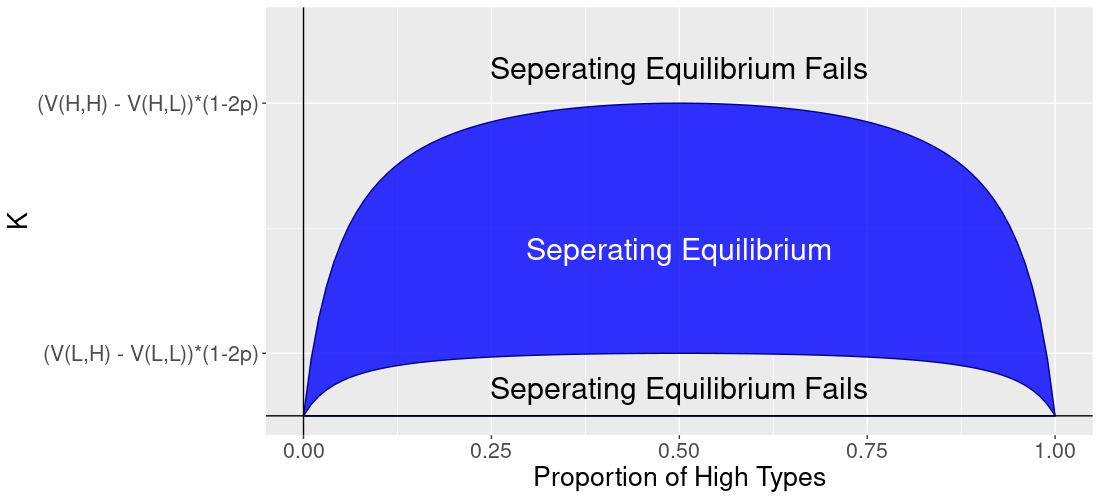
\includegraphics[width=\textwidth, height=.28\textheight]{Images/EquilibriumType3.png}
    \end{figure}
 
Note that since $1-\frac{S^L*p}{S^H*(1-p)+S^L*p}-\frac{S^H*p}{S^H*p+S^L*(1-p)} \in (0,1]$ inequality [\ref{imperfectsignaldynamic13}] implies that in order for a separating equilibrium with signaling cost $K$ to exist, it must be the case that: \begin{equation}
     V(H,H)+V(L,L)>V(L,H)+V(H,L).
 \end{equation}
 This, is the same single crossing property that was derived when populations signal with perfect accuracy. \citep{Zahavi1975, Spence1973}.

As in the case of perfect signaling, imperfect signaling can improve short run population growth through imperfect assortative matching resulting in faster evolution of the type makeup of a population. Unlike the case of perfect signaling, once the population is nearly entirely high types, the population no longer signals by choice, only signaling by mistake with probability $p$. However, this $p*K$ cost of signaling means that the non-signaling population will always, in the long run, attain a higher reproductive rate and larger population, just like in the case of perfect signaling. In examining how imperfect signaling might impact competition, Figure \ref{fig:IFight} provides three examples of outcomes when conflicts occur in our model, using the same initial parameters used in figure \ref{fig:Fight}, but here with a 5\% chance of making a mistake when signaling, that is, $p =0.05$. As can be seen, the margins between the populations in figure \ref{fig:IFight} become slimmer than in figure \ref{fig:Fight}, however, the same patterns remain. The imperfect signaling population may gain an advantage initially and if competition occurs, can defeat the non-signaling population. However, given enough time to evolve before conflict, the non-signaling population will always win.
\begin{figure}[p]
  \caption{Conflicts Between Imperfect Signaling and Non-Signaling Populations After a Period of Peace}
   \label{fig:IFight}
    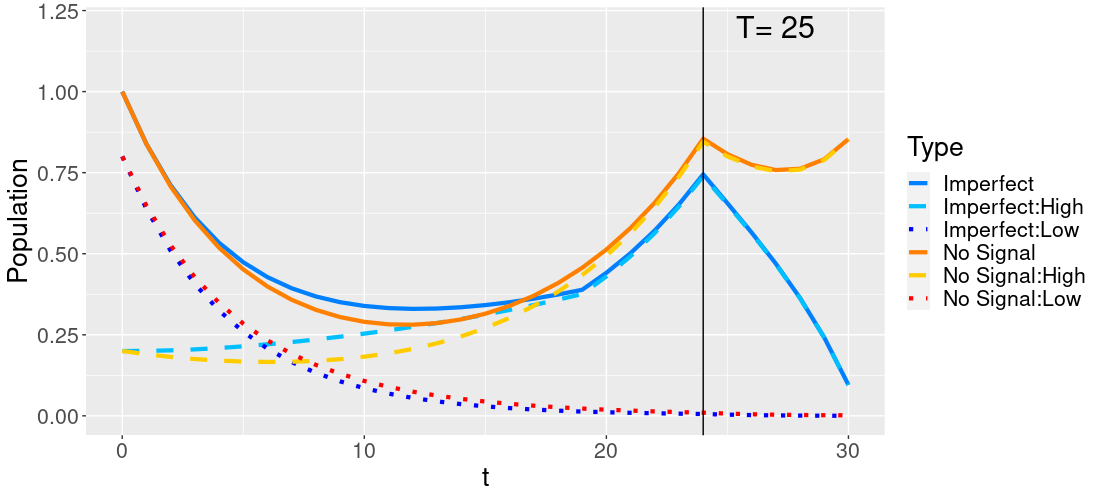
\includegraphics[width=\textwidth, height=.28\textheight]{Images/Fight_I_NS_Win.png}
    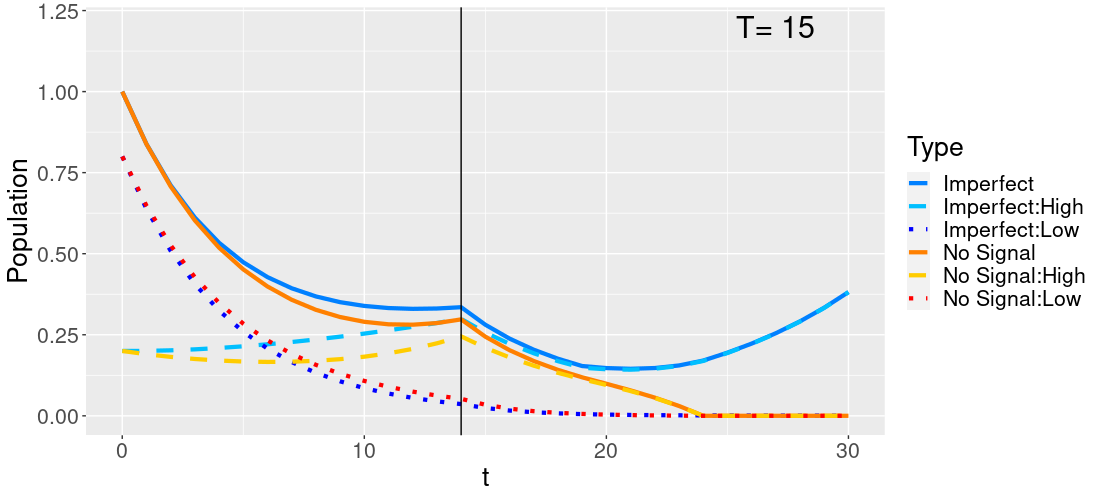
\includegraphics[width=\textwidth, height=.28\textheight]{Images/Fight_I_S_Win.png}
    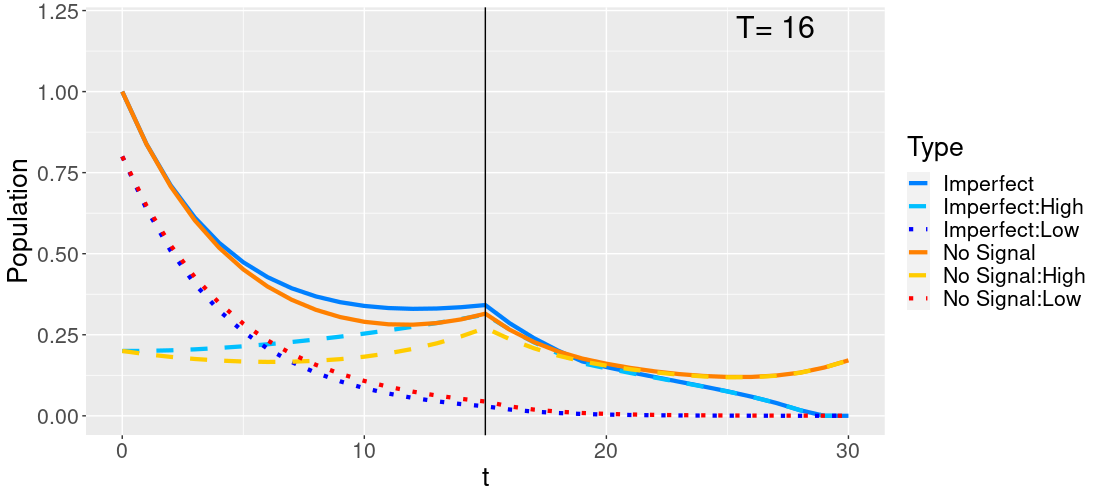
\includegraphics[width=\textwidth, height=.28\textheight]{Images/Fight_I_Special.png}
 \begin{minipage}[c]{.2\textwidth}
    \textbf{Parameters:}
    \end{minipage}\hfill
    \begin{minipage}[c]{.2\textwidth}
    
    $N_0^H = S_0^H = .2$
    
    $N_0^L = S_0^L = .8$
    
    $K = .1$
    
    $\beta = .2$

    $p = .05$
    \end{minipage}\hfill
  \begin{minipage}[c]{.3\textwidth}
  \begin{tabular}{cc|c|c|}
      & \multicolumn{1}{c}{} & \multicolumn{1}{c}{H}  & \multicolumn{1}{c}{L} \\\cline{3-4}
      \multirow{2}*{}  & H & $1.15$ & $0.90$ \\\cline{3-4}
      & L & $0.85$ & $0.80$ \\\cline{3-4}
    \end{tabular}
    \end{minipage}\hfill
    \begin{minipage}[c]{.3\textwidth}
    The vertical lines indicate the last period before conflicts begin $(T-1)$.
    \end{minipage}
    \end{figure} 


\subsection{Concluding Remarks}

It has been well understood that costly signaling can provide a competitive advantage at the intra-group level, however, to our knowledge the effects of signaling has not been examined at the inter-group level of conflicts. We consider a model in which the same individuals (high types) that benefit from signaling would evolve even in the absence of signaling. Thus, when there are two populations, one with and one without signaling, it follows that they would both eventually evolve to be homogeneously high type. At that point, if the two populations were to engage in conflicts, the population without signaling would have a competitive advantage because they do not need to pay the cost of signaling. However, we argue that there can be an advantage to signaling in inter-group conflicts: that the group with signaling evolves faster than the group without signaling. As a result, if conflicts occur, the prevailing population is largely a question of how long the populations evolve in isolation before they engage in conflicts. Our model predicts that societies that have shorter periods of isolation before conflicts, and more efficient weapon used in conflicts may favor the rise of signaling norms. 


%--- Chapter 5 ----------------------------------------------------------------%
\chapter{Conclusion}
\section{Chapter Four Section One}
\subsection{Chapter four section one sub-section one}
\subsubsection{Chapter four section one sub-section one sub-sub-section one}

